% Preamble
% ---
\documentclass[paper=a4, fontsize=11pt]{scrartcl}

% Packages
% ---
\usepackage{geometry}
\geometry{
  a4paper,
  left=15mm,
  right=15mm,
  headheight=50mm,
  top=30mm,
  bottom=16mm,
  footskip=10mm
}
\usepackage{graphicx}
\usepackage[utf8]{inputenc}     % UTF-8 support
\usepackage{amsmath,amsfonts}   % Advanced math typesetting
\usepackage{gauss}              % Matrices reduction operations
\usepackage{lastpage}           % Reference to last page
\usepackage[parfill]{parskip}   % No indent at start of new line
\usepackage{hyperref}           % Table of contents with clickable links
\usepackage{subfig}             % Figure repartition on page
\usepackage{ragged2e}
\usepackage[T1]{fontenc}
\usepackage[french]{babel}
\usepackage{listings}           % Source code formatting and highlighting
    \lstdefinestyle{ascii-tree}{% Tree command Linux
        literate={├}{|}1 {─}{--}1 {└}{+}1 
    }
\usepackage{float}              % Positioning of figures
\usepackage{multirow,tabularx}
\usepackage{xcolor}             % Color in code blocks
\usepackage[toc,page]{appendix} % Reference to appendix
\usepackage{amssymb}            % Special symbols
\usepackage{csquotes}
\usepackage{biblatex}           % Bibliography
\addbibresource{biblio/bibliography.bib}

\pagenumbering{roman}

\newcommand{\ts}{\textsuperscript} % shortcut


% Code Block style
\definecolor{codegreen}{rgb}{0,0.6,0}
\definecolor{codegray}{rgb}{0.5,0.5,0.5}
\definecolor{codepurple}{rgb}{0.58,0,0.82}
\definecolor{backcolour}{rgb}{0.95,0.95,0.92}
\lstdefinestyle{mystyle}{
    backgroundcolor=\color{backcolour},   
    commentstyle=\color{codegreen},
    keywordstyle=\color{magenta},
    numberstyle=\tiny\color{codegray},
    stringstyle=\color{codepurple},
    basicstyle=\ttfamily\footnotesize,
    breakatwhitespace=false,         
    breaklines=true,                 
    captionpos=b,                    
    keepspaces=true,                 
    numbers=left,                    
    numbersep=5pt,                  
    showspaces=false,                
    showstringspaces=false,
    showtabs=false,                  
    tabsize=2
}
\lstset{style=mystyle}

\frenchbsetup{StandardLists=true}
\hypersetup{
    colorlinks,
    citecolor=black,
    filecolor=black,
    linkcolor=black,
    urlcolor=black
}
\usepackage{fancyhdr}           % Create headers and footers
\pagestyle{fancy}

% Header and footer things
% ---
% Header of all pages
\lhead{
\includegraphics[width=5cm]{img/logo.png}}
\rhead{Jael Dubey\linebreak Confidentiel}

% Footer of all pages
\renewcommand{\footrulewidth}{0.4pt}
\lfoot{Système de logging multi-niveau}
\cfoot{}
\rfoot{\textbf{\thepage}}

% Header and footer of the first page
\fancypagestyle{firstpage}{
  \renewcommand{\headrulewidth}{0pt}
  \lhead{
\includegraphics[width=5cm]{img/logo.png}}
  \chead{}
  \rhead{Département : Technologies de l'information et de la communication\linebreak Filière : Informatique et systèmes de communication\linebreak Orientation : Informatique logicielle}
  \renewcommand{\footrulewidth}{0pt}
  \lfoot{}
  \rfoot{}
}


% Modify the \paragraph behavior
\makeatletter
\renewcommand\paragraph{\@startsection{paragraph}{4}{\z@}%
            {-2.5ex\@plus -1ex \@minus -.25ex}%
            {1.25ex \@plus .25ex}%
            {\normalfont\normalsize\bfseries}}
\makeatother
\setcounter{secnumdepth}{4} % how many sectioning levels to assign numbers to
\setcounter{tocdepth}{4}    % how many sectioning levels to show in ToC


% Document
% ---
\begin{document}

% Don't number sections
% \setcounter{secnumdepth}{0}

% Title page ========================================================
\begin{titlepage}
  \thispagestyle{firstpage}
  \begin{center}
    \vspace*{5cm}
    
    \Huge
    \textbf{Travail de Bachelor}
    \large
    \\

    \vspace{1.2cm}
    \LARGE
    Analyse et implémentation d'un système de logging multi-niveau pour une plateforme Smart Grid
  \end{center}

  \vspace{6cm}
  \begin{tabbing}
    \linespread{3}\textbf{Étudiant :} \hspace{12em} \= Jael Dubey\\\\

    \textbf{Travail proposé par :} \> Jonathan Bischof\\
    \> DEPsys SA\\
    \> Route du Verney 20B\\
    \> 1070 Puidoux\\\\

    \textbf{Enseignant responsable :} \> Dr Nastaran Fatemi\\\\

    \textbf{Année académique :} \> 2019-2020
  \end{tabbing}

  \vspace{3cm}
  \begin{flushright}
    Yverdon-les-Bains, le 31 juillet 2020
  \end{flushright}
\end{titlepage}

\newpage
\addcontentsline{toc}{section}{Résumé publiable}

\begin{flushright}
      Département : TIC\\
      Filière : Informatique et systèmes de communication\\
      Orientation : Informatique logicielle\\
      Étudiant : Jael Dubey\\
      Enseignant responsable : Nastaran Fatemi\\
  \end{flushright}
  
  \vspace{0.6cm}
  
  \begin{center}
      {\large Travail de Bachelor 2019-2020 \\[0.2cm]}
      {Analyse et implémentation d’un système de logging multi-niveau pour une plateforme Smart Grid\\[0.5cm]}
  \end{center}
  
  \hrule
  \vspace{0.5cm}
  
  {Nom de l'entreprise/institution}

  DEPsys SA

  \vspace{0.5cm}
  
  {\bfseries Résumé publiable}
  
  {Dans le paysage informatique actuel, passé et très probablement futur, quasiment tous les programmes génèrent des logs, ou journaux en français. Ces logs sont bien souvent oubliés, ou simplement stockés automatiquement dans un fichier qui tombera lui aussi dans l'oubli. Les logs sont en effet très pénibles à lire pour un humain, ils se ressemblent et parfois contiennent une partie incompréhensible, comme des codes numériques.\newline
  Par contre, un travail de lecture d'informations qui se ressemblent est totalement adapté à un ordinateur. C'est pourquoi il existe des logiciels appelés \og système de gestion de logs \fg, dont le but est de lire les informations contenues dans les logs et d'en faire des visualisations agréables à utiliser. L'objectif ce Travail de Bachelor était d'étudier ces différents systèmes afin d'en choisir un, puis de le déployer dans une plateforme Smart Grid.\newline
  Pour ce faire, une évaluation des différents systèmes actuellement utilisés dans le monde a d'abord permis de choisir un outil adapté à notre projet. Ensuite, un déploiement a été fait avec les outils Docker et Docker-Compose. Enfin, une recherche a été effectuée sur les différents algorithmes et techniques utilisés afin de soutirer encore plus d'information à ces logs. En effet, un journal en soi véhicule déjà une information, mais en mettant en relation plusieurs logs, il est possible d'anticiper des problèmes, ou encore de détecter des problèmes complexes de manière automatique. \newline
  Dans ce Travail de Bachelor, le programme qui a été choisi lors de l'évaluation est la Suite Elastic. Une architecture fonctionnelle et facilement déployable a ensuite été créé. Pour finir, des recherches sur les algorithmes actuellement utilisés dans ce domaine ont expliqué les fonctionnalités de chacun, puis une implémentation a montré les capacités de ces algorithmes.}

  
  \begin{figure}[H]
    \centering
    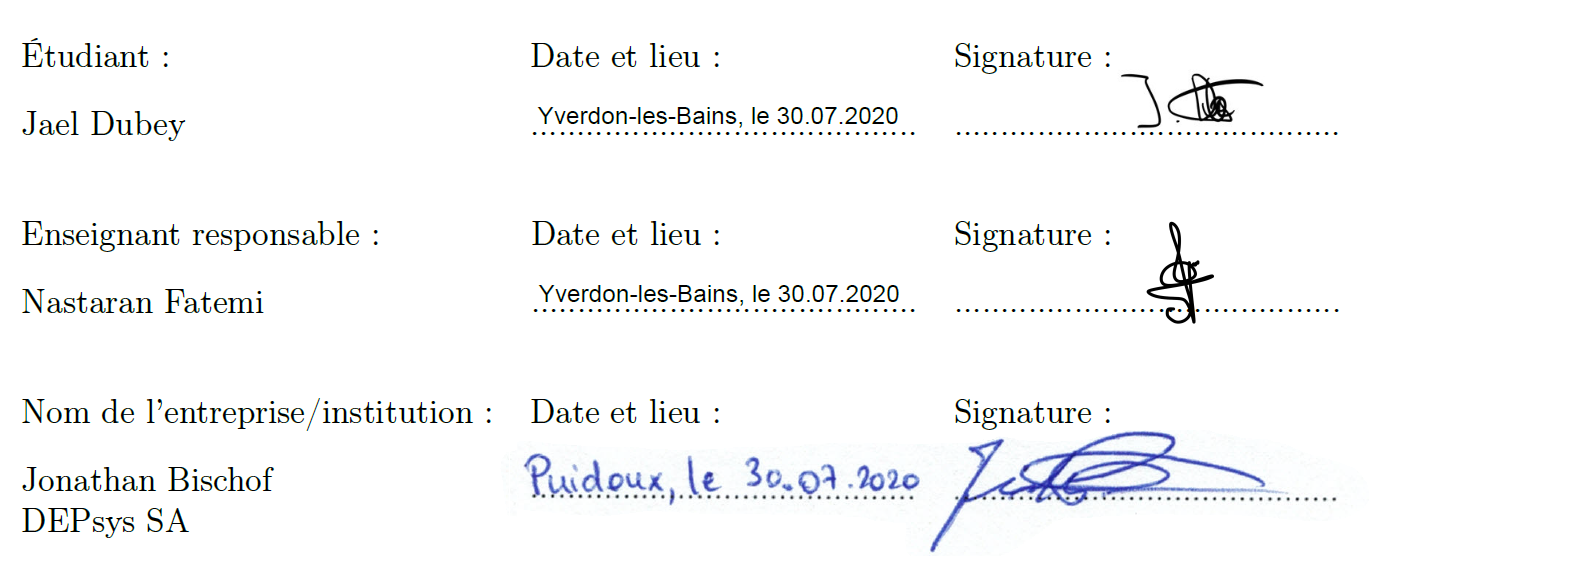
\includegraphics[width=18cm]{img/signatures_resume.png}
    \label{f-signatureJaelNastJonathan}
  \end{figure}
  
  
%  \begin{tabular}{lll}
%      Étudiant : & Date et lieu : & Signature :  \\[0.3cm]
%      {Jael Dubey} & .......................................... &  %.......................................... \\[0.8cm]
%      Enseignant responsable : & Date et lieu : & Signature :  \\[0.3cm]
%  
%      {Nastaran Fatemi} & .......................................... &  %.......................................... \\[0.8cm]
%      Nom de l'entreprise/institution : & Date et lieu : & Signature :  \\[0.3cm]
%  
%      {Jonathan Bischof} & .......................................... &  %.......................................... \\
%      {DEPsys SA}
%  \end{tabular}
  
\newpage

\addsec{Préambule}
  
  Ce travail de Bachelor (ci-après TB) est réalisé en fin de cursus d’études, en vue de l'obtention du titre de Bachelor of Science HES-SO en Ingénierie. \\
  
  En tant que travail académique, son contenu, sans préjuger de sa valeur, n'engage ni la responsabilité de l'auteur, ni celles du jury du travail de Bachelor et de l'Ecole. \\
  
  Toute utilisation, même partielle, de ce TB doit être faite dans le respect du droit d’auteur. \\
  
  
  \begin{flushright}
      \begin{minipage}{7cm}
          \vspace{2cm}
          HEIG-VD \\
  
          \vspace{2cm}
  
          Vincent Peiris\\
          Chef de département TIC
      \end{minipage}\hfill
  \end{flushright}
  
  \vspace{3cm}
  
  Yverdon-les-Bains, le 31 juillet 2020
  
  \newpage
  
\addsec{Authentification}

Le soussigné, Jael Dubey, atteste par la présente avoir réalisé seul ce travail et n’avoir utilisé aucune autre source que celles expressément mentionnées.

\vspace{2cm}

\noindent {Yverdon-les-bains}, le 31 juillet 2020

\vspace{3cm}

\begin{flushright}
    \begin{minipage}{7cm}
        {Jael Dubey}
    \end{minipage}\hfill
\end{flushright}

\newpage

% Cahier des charges ================================================
\addsec{Cahier des charges}
\subsection*{Résumé du problème}
DEPsys est une entreprise Suisse leader technologique du marché énergétique. Fondée en 2012 et basée à Puidoux, elle fournit des solutions évolutives basées sur sa plateforme GridEye permettant aux réseaux de distribution d'énergie traditionnels de faire face aux nouvelles contraintes de la production décentralisée des sources d'énergie renouvelable, tels que les systèmes photovoltaïques et les technologies de mobilité électrique.

La plateforme GridEye offre une solution technologique innovatrice pour les gestionnaires de réseau de distribution (GRD, p. ex. Romande Énergie). Positionné de manière unique avec sa simplicité de déploiement, c'est la seule solution réellement Plug \& Play qui évite tous les problèmes d'installation. La surveillance du réseau électrique en temps réel et les statistiques fournissent des informations détaillées sur les conditions du réseau. Les algorithmes de contrôle et de gestion garantissent la qualité et la stabilité du réseau.

Ce Travail de Bachelor consiste en une évaluation de différentes technologies de logging et de l'analyse des performances, pour ensuite mettre en place la meilleure solution pour l'infrastructure GridEye.

\subsection*{Étapes de réalisation du projet}

\begin{itemize}
    \item Étude des systèmes de gestion de logs actuels.
    \subitem Choix des systèmes à évaluer.
    \item Évaluation théorique des systèmes.
    \item Prise en main et configuration des outils pour une comparaison théorique \& pratique.
    \subitem Choix d'un système.
    \item Implémentation d'un cas d'utilisation concret fourni par DEPsys.
    \subitem Avec un programme de simulation minimaliste de la plateforme GridEye.
    \item Implémentation d'une démonstration de faisabilité (Proof of Concept, PoC).
    \item Implémentation de librairies (SDK) pour l'interfaçage avec le Back-End de la solution GridEye (puis Front-End, puis outils externes).
\end{itemize}

\subsection*{Informations diverses et technologies}
Les logs sont constitués de plusieurs types (System, User Action, Notification, ...) avec différents niveaux de priorités (debug, info, ...). Les logs utilisateurs doivent pouvoir être consultés depuis le Front-End, alors que les logs systèmes peuvent être accessible depuis une dashboard interne. Les notifications, dépendant du niveau de priorité, doivent pouvoir être transmises en temps réel aux gestionnaire de réseau de distribution électrique  par e-mail, notification push, etc. ou sous forme de rapport journalier/hebdomadaire. La mise en place de librairies (SDK) est nécessaire pour communiquer avec les différents composants de l'infrastructure. Le but étant de pouvoir s'interfacer avec l'infrastructure actuelle afin de pouvoir remplacer la solution de logging actuelle.

Technologies:

\begin{itemize}
    \item Base de données : SQL, JSON, ... (dépendant de la solution choisie).
    \item Back-End : Java
    \item Front-End : Javascript 
    \item Outils externes : Python 3
\end{itemize}
\newpage

% Contents page =====================================================
\renewcommand{\contentsname}{Table des matières}
\tableofcontents

\newpage
\pagenumbering{arabic}
\rfoot{Page \textbf{\thepage} \ sur \textbf{\pageref{LastPage}}}
% Document start ====================================================
\addtocontents{toc}{\protect\setcounter{tocdepth}{5}}
\section{Introduction}

La plateforme GridEye de DEPsys \cite{noauthor_depsys_nodate} est une solution permettant d'optimiser les réseaux électriques. Elle s'adresse aux gestionnaires de réseau de distribution, et permet de faire face aux contraintes de la production décentralisée, qui correspondent par exemple aux panneaux photovoltaïques, ou encore aux batteries de stockage. Autant d'équipements que de plus en plus de particulier se procurent, tout autant que les entreprises. Cette transition énergétique est accélérée en Suisse avec la \og Stratégie Energétique 2050 \fg \cite{noauthor_detec_nodate}, un texte de loi accepté par le peuple en 2017, qui promeut les énergies renouvelables.

Concrètement, GridEye est une solution qui peut se greffer à tout système déjà existant, ce qui évite tous les problèmes liés à l'installation. GridEye permet une optimisation efficace du réseau grâce à plusieurs applications, ayant principalement pour but d'assurer une grande qualité et une haute fiabilité. Ces qualités sont atteintes avec des outils de surveillance du réseau, d'analyses des événements via des algorithmes sophistiqués, et d'autres fonctionnalités diverses. Le service de GridEye fourni également l'accès à tout un support hautement qualifié. La figure \ref{f-GridEyeDescription} montre les différentes applications de GridEye, ainsi que ses composants et services.

\begin{figure}[H]
    \centering
    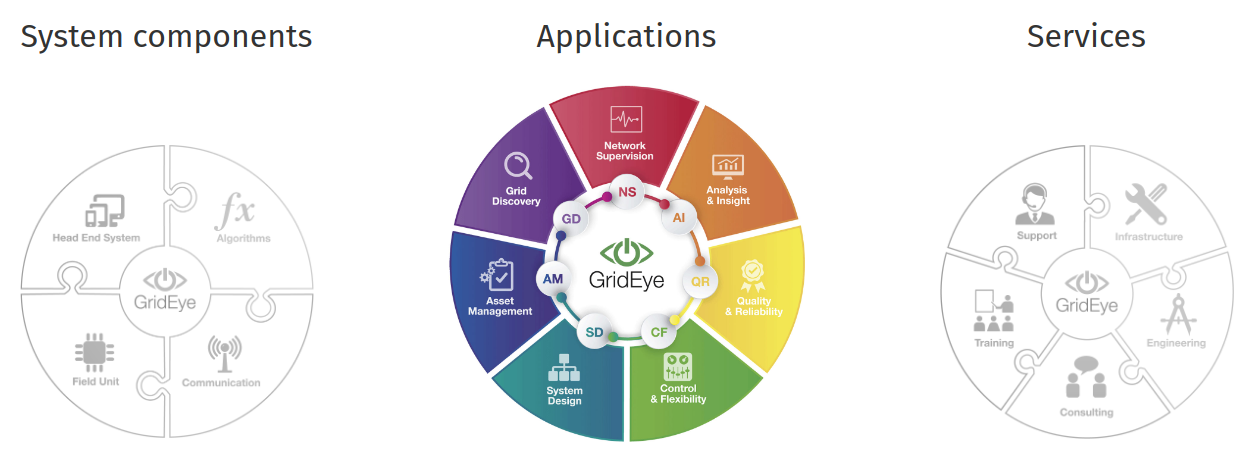
\includegraphics[width=18cm]{img/screenshots/GridEye.png}
    \caption{Description de la plateforme GridEye \cite{noauthor_depsys_nodate}}
    \label{f-GridEyeDescription}
\end{figure}

Ce Travail de Bachelor se positionne dans les applications d'analyse et de surveillance du réseau électrique. Le but est, à terme, de remplacer la solution actuelle par un système de gestion de logs. Ce but sera atteint à travers plusieurs étapes. Tout d'abord, il s'agira de réaliser une étude de l'état de l'art en matière de système de gestion de logs. Il faudra voir quels sont les logiciels les plus utilisés actuellement et juger leurs qualités ou inconvénients respectifs. Cette étude permettra de choisir quelques systèmes à évaluer. L'évaluation de ces systèmes consistera en une recherche approfondie de leurs capacités et fonctionnalités théoriques, puis d'une prise en main et d'un essai concret de chacun. Après toutes ces investigations et considérations, il sera possible de prendre une décision de manière convaincue quant au logiciel à utiliser pour le futur de la plateforme GridEye.
Après avoir fait le choix de l'outil, il faudra s'assurer de sa pertinence dans notre domaine de travail au travers de l'implémentation d'un cas d'utilisation se rapprochant de la réalité. Cette implémentation pourra être vue comme une démonstration de faisabilité.
Cette étape supplémentaire pourra, dans le meilleur des cas, nous conforter dans notre choix basé sur les prises en main et fonctionnalités théoriques, ou alors, dans le cas contraire, nous faire changer d'avis et nous raviser sur un autre choix.

Dans tous les cas, le choix sera ici clairement défini et nous pourrons nous lancer dans un développement plus effectif, qui sera utilisé dans l'infrastructure GridEye. Il sera possible de développer des algorithmes permettant de détecter efficacement des anomalies dans le réseau, et si possible de les prévoir, afin de toujours assurer une fiabilité aussi souveraine que possible. Il faudra finalement interfacer la nouvelle solution avec la solution GridEye actuelle.

\newpage

\section{Comparaison des outils}

\subsection{Critères de comparaison}

Pour réaliser une évaluation de différents système de gestion de log, il faut obligatoirement choisir des critères de comparaison. Ces critères se basent sur deux sources. La première étant les demandes formulées par DEPsys, et la deuxième provient des différentes fonctionnalités nécessaires à un système de gestion de logs \cite{noauthor_what_nodate} \cite{noauthor_gestion_2019}. Voici les critères retenus :

\begin{itemize}\itemsep0pt \parskip0pt \parsep0pt
\item La collecte des logs
\subitem Approche minimaliste ou maximaliste, est-ce que le système installe un agent sur le dispositif émetteur de log qui lui envoie uniquement les informations les plus importantes (approche minimaliste, méthode PUSH), ou est-ce que le système reçoit tous les logs et les enregistre tous (approche maximaliste, méthode PULL) ?\\
\item L'agrégation centralisée des logs
\subitem L'agrégation des logs est un défi, car après avoir collecté les logs, il faut tous les regrouper dans un même endroit, alors qu'ils peuvent avoir des formats différents. De plus, ils peuvent être généré très rapidement (s'exprime en EPS, Event Per Second), il faut donc être capable de traiter et regrouper ces logs de manière efficace.\\
\item Le stockage à long terme et la durée de rétention des logs
\subitem Après avoir agrégé ces informations, il faut maintenant faire des choix quant à leur stockage. L'idéal serait de garder tous les logs indéfiniment, mais chaque information stockée a un coût. Il faut donc avoir une stratégie de rétention qui permette de supprimer ou garder tel type de log.\\
\item La rotation des fichiers de logs
\subitem La rotation consiste à rendre automatique la stratégie de rétention et/ou de stockage des logs.\\
\item L'analyse des logs (en temps réel et en vrac après une période de stockage)
\subitem L'analyse des logs est, en quelque sorte, le but de tout le système de gestion de logs. En effet, il ne sert à rien de stocker de l'information sur un système si l'on en fait rien. L'analyse est donc la pour synthétiser les informations contenues dans les logs.\\
\item Les rapports
\subitem Il doit être possible pour un système de gestion des logs d'effectuer des recherches sur les informations stockées et de rédiger des rapports.\\
\item Visionnage et gestion des alertes
\subitem Un des buts d'un système de gestion de logs est de pouvoir réagir très vite à un problème, voire même de l'anticiper. Ceci passe par une émission d'alerte et d'une possibilité de visionnage des données, si possible en temps réel.\\
\item Popularité
\subitem Voici un critère qui change en permanence, mais qui a son importance lors d'un choix d'outil informatique. En effet, un logiciel sur le déclin sera de plus en plus dur à supporter, alors qu'un outil trop jeune n'a souvent que trop peu d'utilisateurs qui pourraient partager leurs connaissances sur les forums. L'idéal étant donc un logiciel populaire et qui est en pleine croissance.
\end{itemize}

En plus de ces critères, les coûts d'utilisation seront, si possible, évalués.\\

\subsection{Choix des différents systèmes à évaluer}

Comme pour le choix des critères de comparaison, les différents systèmes qui vont être analysés ont été définis soit par DEPsys, soit par des recherches dans les nombreux classement de \og Log Management Tools \fg disponibles sur internet.\\
Quatre classements différents ont été sélectionnés afin d'avoir plusieurs avis différents, tout en restant dans une quantité raisonnable d'analyses. Les classements qui allaient être utilisés devaient être neutres. On entend par là que le site réalisant le classement ne doit pas proposer, par exemple, une solution cloud utilisant un certain outil de gestion de log, auquel cas son classement serait forcément biaisé. Il fallait également que le classement soit récent, étant donné la vitesse d'évolution générale des outils informatiques. Une période d'un an maximum a été définie.\\\\
Les classements suivants ont été choisis :
\begin{itemize}
    \item Top 8 BEST Log Management Software \cite{noauthor_top_nodate}
    \subitem Classement datant de mars 2020, et publié par \textit{SoftwareTestingHelp}.
    \item Best Log Manager \& Monitoring Software \& Tools \cite{noauthor_best_nodate}
    \subitem Classement datant de janvier 2020, et publié par \textit{iTT Systems}.
    \item 6 Best Log Management Tools \cite{noauthor_6_2019}
    \subitem Classement datant de août 2019, et publié par \textit{AddictiveTips}.
    \item 13 Best Log Management \& Analysis Tools \cite{says_ten_2019}
    \subitem Classement datant de août 2019, et publié par \textit{Comparitech}.
\end{itemize}

Les quatre sites internet retenus sont de simples portails informatiques, publiant des articles sur divers sujets informatiques. Lorsque l'on effectue une recherche Google \cite{noauthor_google_nodate-1} afin de trouver des classements de système de gestion de logs, on tombe régulièrement sur des articles de \textit{DNSStuff} \cite{noauthor_dnsstuff_nodate} et \textit{Sematext} \cite{noauthor_sematext_nodate}. Ceux-ci n'ont pas été utilisé car le premier appartient à SolarWinds \cite{noauthor_logiciels_nodate}, une entreprise proposant plusieurs logiciels, dont des systèmes de gestion de logs, et le second propose des solutions cloud utilisant des outils de gestion de logs. Ils ont donc été jugés non-neutre.

Afin de réaliser un classement regroupant le contenu de ces 4 tops, une note a été attribuée à chaque position de chaque classement. Deux critères ont été intégré dans le calcul de la note : la position (mieux on est positionné dans son propre classement, plus on aura de points), ainsi que le nombre total d'outils cités. Il est en effet plus facile d'être bien classé dans un classement contenant 5 outils que dans un classement en contenant 10. Pour finir, afin de faciliter la lecture, la note attribuée se situe entre 0 (le plus mauvais), et 100 (la meilleure note possible). La formule suivante a donc été appliquée :
\[\frac{i * 100}{n}\]
i étant la position dans le classement, et n le nombre total d'outils dans le classement.\\

Les tableaux \ref{table-Classement1} et \ref{table-Classement2} montrent les points obtenus par chaque système.

\begin{table}[H]
\centering
\subfloat[Classement de SoftwareTestingHelp]{\begin{tabular}{ |p{6cm}|p{1cm}|  }
     \hline
     \multicolumn{2}{|c|}{SoftwareTestingHelp} \\
     \hline
     Système & Points\\
     \hline
     SolarWinds Log Analyzer & 100\\
     Sematext Logs & 89\\
     Splunk & 78\\
     ManageEngine EventLog Analyzer & 67\\
     LogDNA & 56\\
     Fluentd & 44\\
     Logalyze & 33\\
     Graylog & 22\\
     Netwrix Auditor & 11\\
     \hline
    \end{tabular}}
\quad
\subfloat[Classement de Comparitech]{\begin{tabular}{ |p{6cm}|p{1cm}|  }
     \hline
     \multicolumn{2}{|c|}{Comparitech} \\
     \hline
     Système & Points\\
     \hline
     ManageEngine EventLog Analyzer & 100\\
     SolarWinds Papertrail & 92\\
     Loggly & 83\\
     PRTG Network Monitor & 75\\
     Splunk & 67\\
     Fluentd & 58\\
     Logstash & 50\\
     Kibana & 43\\
     Graylog & 33\\
     XpoLog & 25\\
     ManageEngine SyslogForwarder & 17\\
     TekWire Managelogs & 8\\
     \hline
    \end{tabular}}
    \caption{Classements SoftwareTestingHelp et Comparitech}
    \label{table-Classement1}

\end{table}

\begin{table}[H]
\centering
\subfloat[Classement de AddictiveTips]{\begin{tabular}{ |p{6cm}|p{1cm}|  }
     \hline
     \multicolumn{2}{|c|}{AddictiveTips} \\
     \hline
     Système & Points\\
     \hline
     SolarWinds Papertrail & 100\\
     SolarWinds Loggly & 83\\
     Splunk & 67\\
     Nagios Log Server & 50\\
     Graylog & 33\\
     ManageEngine EventLog Analyzer & 17\\
     \hline
    \end{tabular}}
\quad
\subfloat[Classement de iTT Systems]{\begin{tabular}{ |p{6cm}|p{1cm}|  }
     \hline
     \multicolumn{2}{|c|}{iTT Systems} \\
     \hline
     Système & Points\\
     \hline
     SolarWinds Log \& Event Manager & 100\\
     PRTG Network Monitor & 83\\
     Lepide & 67\\
     McAfee Enterprise Log Manager & 50\\
     Veriato & 33\\
     Splunk & 17\\
     \hline
    \end{tabular}}
    \caption{Classements AddictiveTips et iTT Systems}
    \label{table-Classement2}
\end{table}

Et le tableau \ref{t-classementGlobal} montre le classement global, calculé d'après l'addition des points obtenus dans les différents classements.

\begin{table}[H]
\centering
\begin{tabular}{ |p{2cm}|p{6cm}|p{1cm}| } 
    \hline
     & Système & Points\\
    \hline
    1 & Splunk & 229\\
    2 & SolarWinds Papertrail & 192\\
    3 & ManageEngine EventLog Analyzer & 184\\
    4 & SolarWinds Loggly & 166\\
    5 & PRTG Network Monitor & 158\\
    6 & Fluentd & 102\\
    7 & SolarWinds Log Analyzer & 100\\
    8 & SolarWinds Log \& Event Manager & 100\\
    9 & ELK Stack (Kibana + Logstash)  & 93\\
    10 & Sematext Logs & 89\\
    11 & Graylog & 88\\
    12 & Lepide & 67\\
    13 & LogDNA & 56\\
    14 & Nagios Log Server & 50\\
    15 & McAfee Enterprise Log Manager & 50\\
    16 & Logalyze & 33\\
    17 & Veriato & 33\\
    18 & XpoLog & 25\\
    19 & ManageEngine Syslog Forwarder & 17\\
    20 & Netwrix Auditor & 11\\
    21 & TekWire Managelogs & 8\\
    \hline
\end{tabular}
\caption{Classement global des systèmes de gestion de log}
\label{t-classementGlobal}
\end{table}
\justify

Après une étude légèrement plus approfondie sur ces différents systèmes, il a été décidé de garder les suivants pour la comparaison :

\begin{enumerate}
    \item Elastic Stack \cite{noauthor_recherche_nodate}
    \subitem Choisi par DEPsys, probablement la plus populaire.
    \item Splunk \cite{noauthor_siem_nodate}
    \subitem 1\up{er} du classement.
    \item SolarWinds Loggly \cite{noauthor_log_nodate}
    \subitem De tous les outils appartenant à SolarWinds, je voulais n'en choisir qu'un. Loggly me paraissaît le plus approprié au cas d'utilisation de ce travail de Bachelor.
    \item Graylog \cite{noauthor_industry_nodate}
    \subitem Suggéré par DEPsys, et semble avoir une bonne documentation.
\end{enumerate}

\subsection{Comparaison théorique}
\subsubsection{Elastic Stack}
La \og Elastic Stack \fg, ou \og Suite Elastic \fg en français, anciennement appelée \og ELK Stack \fg est composée de plusieurs outils :
\begin{itemize}
    \item Elasticsearch \cite{noauthor_elasticsearch_nodate}
    \subitem Un moteur de recherche RESTful.
    \item Kibana \cite{noauthor_kibana_nodate}
    \subitem Un outil de visualisation.
    \item Logstash \cite{noauthor_logstash_nodate-1}
    \subitem Un pipeline d'ingestion de log.
    \item Beats \cite{noauthor_agents_nodate}
    \subitem Une famille d'agent dédié au transfert de données.
\end{itemize}

La table \ref{t-resumeELK} montre un résumé des fonctionnalités disponibles ainsi que des coûts lié à la Suite Elastic.

\begin{table}[H]
\centering
\begin{tabular}{ |p{4cm}||p{13cm}|  }
    \hline
    \multicolumn{2}{|c|}{Elastic Stack} \\
    \hline
    Collecte & La collecte des logs se fait en approche minimaliste. La suite Elastic contient l'outil Beat, qui est donc une famille d'agent léger. On installe un agent beat (p. ex. Filebeat, Metricbeat, etc.) sur le système générant les logs, et cet agent envoie les données vers le serveur.\\
    \hline
    Agrégation centralisée & Se fait via Logstash. Peux supporter beaucoup d'événements par seconde (> 10'000 EPS). Compatible avec énormément de type de logs. Permet d'analyser et transformer les logs en temps réel. Logstash dispose d'une API permettant de créer nos propres plug-in, si les sources de données ne sont pas compatible nativement.\\
    \hline
    Stockage et rétention & Le stockage se fait avec Elasticsearch. Il n'y a pas de rétention des données de bases avec Elasticsearch. Il est cependant possible de le faire avec Elastic-Curator, qui est un outil permettant de gérer un cluster Elasticsearch.\\
    \hline
    Rotation & La rotation se fait avec Elastic-Curator\\
    \hline
    Analyse & Elasticsearch et ses requêtes poussées permettent de faire des recherches avancées.\\
    \hline
    Rapport & Les rapports peuvent être générés depuis Kibana.\\
    \hline
    Visionnage et alertes & La visualisation des données en temps réels peut se faire avec Kibana. La gestion des alertes se fait également via Kibana. Il est possible de paramétrer des alertes classiques, qui se déclenchent suivant des règles précises. Et il est également possible de paramétrer des alertes suivant un algorithme d'apprentissage automatique, qui détectera des événements inhabituels.\\
    \hline
    Popularité & La suite Elastic est très certainement la plus populaire actuellement. Elle bénéficie d'une grande communauté active. Au niveau de la tendance, on peut voir une grande croissance entre les années 2016 et 2019. Ces derniers mois, cela semble se stabiliser.\\
    \hline
    Coûts &  La suite Elastic propose différents abonnements. Il y a une offre gratuite, mais celle-ci ne contient pas de gestion d'alerte et de création de rapport. Les prix pour les offres payantes ne sont pas publics. Il faut contacter Elastic et les prix varient en fonction de la taille du système à implémenter.\\
    \hline
\end{tabular}
\caption{Résumé théorique de Elastic Stack}
\label{t-resumeELK}
\end{table}

\subsubsection{Graylog}
Graylog un outil de gestion de logs. Il dispose de deux versions : Open Source et Enterprise. La table \ref{t-resumeGraylog} montre les fonctionnalités du systèmes Graylog.

\begin{table}[H]
\centering
\begin{tabular}{ |p{4cm}||p{13cm}|  }
    \hline
    \multicolumn{2}{|c|}{Graylog} \\
    \hline
    Collecte & La collecte des logs se fait en approche minimaliste. Graylog possède un outil appelé \og Sidecar \fg qui permet de gérer plusieurs type d'agent, y compris l'outil Beat de la suite Elastic.\\
    \hline
    Agrégation centralisée & Graylog permet de gérer \og d'énormes \fg jeux de donnée et de les traiter selon des règles définies par l'utilisateur. En plus des règles d'agrégation classiques, comme l'origine géographique, le niveau d'alerte, etc., Graylog permet de faire des listes noires de logs.\\
    \hline
    Stockage et rétention & Le stockage se fait avec MongoDB et Elasticsearch. Graylog offre une solution (Graylog Archive) de rétention des données, disponible avec la version Enterprise, qui peut être paramétrée.\\
    \hline
    Rotation & La rotation se fait avec Graylog Archive.\\
    \hline
    Analyse & Graylog utilisant Elasticsearch, il dispose de ses requêtes poussées permettant de faire des recherches avancées. Graylog possède également son langage de requête, basé sur Apache Lucene.\\
    \hline
    Rapport & La création de rapport est une fonctionnalité de Graylog Enterprise. Il est possible de les configurer depuis l'interface de Graylog.\\
    \hline
    Visionnage et alertes & La visualisation des données en temps réels se fait avec l'interface de Graylog. La gestion des alertes est incluse dans le Graylog de base. Elle permet de définir des alertes selon des règles. Graylog possède également un \og Store \fg proposant, entre autres, des fonctionnalités liées aux alertes, développées par la communauté.\\
    \hline
    Popularité & Graylog n'est pas arrivé très haut de manière générale dans les tops, mais il est en revanche souvent cité. La courbe de tendance de Graylog est en croissance régulière depuis 2008.\\
    \hline
    Coûts &  Graylog propose deux versions : \og Open Source \fg et \og Enterprise \fg. La première est gratuite mais propose quelques fonctionnalités en moins, comme les rapports programmés ou le support technique. Les coûts de la version \og Enterprise \fg ne sont pas disponibles, il faut contacter Graylog. À noter que la version \og Enterprise \fg est gratuite jusqu'à une utilisation de 5 GB par jour.\\
    \hline
\end{tabular}
\caption{Résumé théorique de Graylog}
\label{t-resumeGraylog}
\end{table}


\subsubsection{SolarWinds Loggly}
SolarWinds Loggly un outil de gestion de logs SaaS (Software-as-a-Service, dans le cloud). Il dispose de plusieurs versions, dont une gratuite. La table \ref{t-resumeLoggly} montre les fonctionnalités et des informations sur les coûts de SolarWinds Loggly.

\begin{table}[H]
\centering
\begin{tabular}{ |p{4cm}||p{13cm}|  }
    \hline
    \multicolumn{2}{|c|}{SolarWinds Loggly} \\
    \hline
    Collecte & L'envoi de données à Loggly est relativement simple. La seule contrainte est qu'il s'agisse de texte. Il n'y a pas besoin d'avoir d'agent (envoi de log via un endpoint), mais il est également possible d'en utiliser.\\
    \hline
    Agrégation centralisée & Loggly permet de parser les logs des formats les plus connus, comme les logs MySQL ou Java, mais ne possède pas d'outil permettant de réaliser un filtrage et une agrégation de logs personnalisés. Pour ce faire, il préconise d'utiliser un logiciel comme Logstash. \\
    \hline
    Stockage et rétention & La rétention des données est plutôt courte (7 jours dans la version gratuite), et ensuite, les logs peuvent être sauvegardés dans une instance S3 de AWS.\\
    \hline
    Rotation & La rétention se fait automatiquement après un certain nombre de jour.\\
    \hline
    Analyse & Loggly possède son propre langage de requête, qui est basé sur Apache Lucene. Il est également possible d'analyser les logs en temps réel via l'interface de Loggly.\\
    \hline
    Rapport & Il est possible de réaliser des rapport dans plusieurs format depuis l'interface graphique.\\
    \hline
    Visionnage et alertes & Il est possible de configurer des alertes selon des règles classiques, et également sur des événements inhabituels. Le visionnage des données en direct se fait via l'interface graphique de Loggly.\\
    \hline
    Popularité & Loggly était en croissance entre 2008 et 2016, mais depuis cette année-ci, sa courbe de tendance est en décroissance.\\
    \hline
    Coûts & Loggly propose une version gratuite et trois versions payantes. La version gratuite est limitée à un volume de 200 MB par jour, un seul utilisateur pouvant se connecter sur une instance, et ne contient pas certaines fonctionnalités comme la gestion des alertes. Les versions payantes varient entre 79 et 279 USD par mois, et proposent chacune quelques fonctionnalités en plus, et un volume de moins en moins limité.\\
    \hline
\end{tabular}
\caption{Résumé théorique de SolarWinds Loggly}
\label{t-resumeLoggly}
\end{table}


\subsubsection{Splunk}
Splunk est un outil de gestion de logs. Il est séparé en trois \og parties \fg, chacune étant responsable de plusieurs choses :

\begin{itemize}
    \item Universal Forwarder
    \subitem Effectue la collecte et envoie les données à l'indexer.
    \item Indexer
    \subitem Effectue le stockage des logs.
    \item Search Head
    \subitem Permet de lire dans l'index.
\end{itemize}
Chacune de ces fonctions peut être transformé en cluster si de grand volume de données sont à traiter.
Splunk peut être disponible en version \og sur site \fg ou \og cloud \fg. La table \ref{t-resumeSplunk} montre les fonctionnalités et les coûts relatifs à Splunk.

\begin{table}[H]
\centering
\begin{tabular}{ |p{4cm}||p{13cm}|  }
    \hline
    \multicolumn{2}{|c|}{Splunk} \\
    \hline
    Collecte & La collecte des logs se fait en approche minimaliste. Ceci via les \og Universal Forwarder \fg qui sont des agents à installer sur le système générant les logs. Il envoie ensuite les données vers l'indexer.\\
    \hline
    Agrégation centralisée & Pour Splunk, l'agrégation des logs ne se fait pas dans le pipeline lors de l'ingestion des logs, mais après coup. Cela se fait donc une fois que les logs ont été indexés. Il est possible de faire des filtres personnalisés ainsi que d'utiliser des filtres pour les formats courants, et ceci avec une fonctionnalité s'appelant \og Field Extraction \fg.\\
    \hline
    Stockage et rétention & Le stockage des logs se fait avec l'indexer. Concernant la rétention des données, Splunk la gère avec des \og buckets \fg. Concrètement, un bucket possède une durée qui détermine le temps qu'une donnée va passer dedans. P. ex., on peut avoir un bucket de 30 jours où les logs seront accessible et analysable librement. Puis, passé ces 30 jours, ils iront dans un autre bucket où ils seront compressé pour le stockage à long terme.\\
    \hline
    Rotation & Se fait via les buckets.\\
    \hline
    Analyse & L'analyse est possible via l'interface de Splunk. Celle-ci permet de trier et filtrer les logs selon de nombreux critères.\\
    \hline
    Rapport & La génération de rapport est possible depuis l'interface de Splunk.\\
    \hline
    Visionnage et alertes & Le visionnage et la gestion des alertes est également possible depuis l'interface de Splunk. Pour les alertes, elles sont définissables selon des règles classiques (p. ex. logs provenant d'une adresse IP particulière, etc.).\\
    \hline
    Popularité & D'après les courbes de Google Trends, le système Splunk est en constante croissance depuis 2010. Dans le classement des différents tops consultés, Splunk arrive en bonne position. Splunk bénéficie d'une documentation relativement grande et d'un forum.\\
    \hline
    Coûts & Les coûts sont en \og infrastructure-based pricing \fg et ne sont donc pas fixe. Mais Splunk Enterprise commence à 150\$ par mois. Splunk ne propose pas de version gratuite (mise à part l'essai de 60 jours).\\
    \hline
\end{tabular}
\caption{Résumé théorique de Splunk}
\label{t-resumeSplunk}
\end{table}

\subsubsection{Popularité des systèmes}

La comparaison de popularité des différents systèmes permet de se faire un idée sur les tendances actuelles et passées d'utilisation de ces systèmes. Elle a également pour but de pouvoir éventuellement anticiper les futures tendances. Ces données sont importantes lors du choix d'un logiciel, afin de pouvoir compter sur un support de la communauté lors des problèmes qui arriveront pendant le développement.

\textbf{Conditions de tests} \\

\begin{itemize}
    \item Les courbes de tendances seront tirées de Google Trends \cite{noauthor_google_nodate}.
    \item Les courbes porteront sur les 10 dernières années.
    \subitem Du 23 avril 2010 au 23 avril 2020
    \item Les courbes porteront sur les recherches dans tous les pays du monde.
    \item Il n'y aura pas d'autre restriction de recherche (catégorie, outil Google)
\end{itemize}

\textbf{Résultats} \\
La figure \ref{f-Trends4Systemes} montre les courbes de tendances des quatre systèmes. Les courbes de Loggly et Graylog étant particulièrement basses et donc difficilement comparable, la figure \ref{f-Trends2Systemes} permet de les comparer entre elles.

\begin{figure}[H]
    \centering
    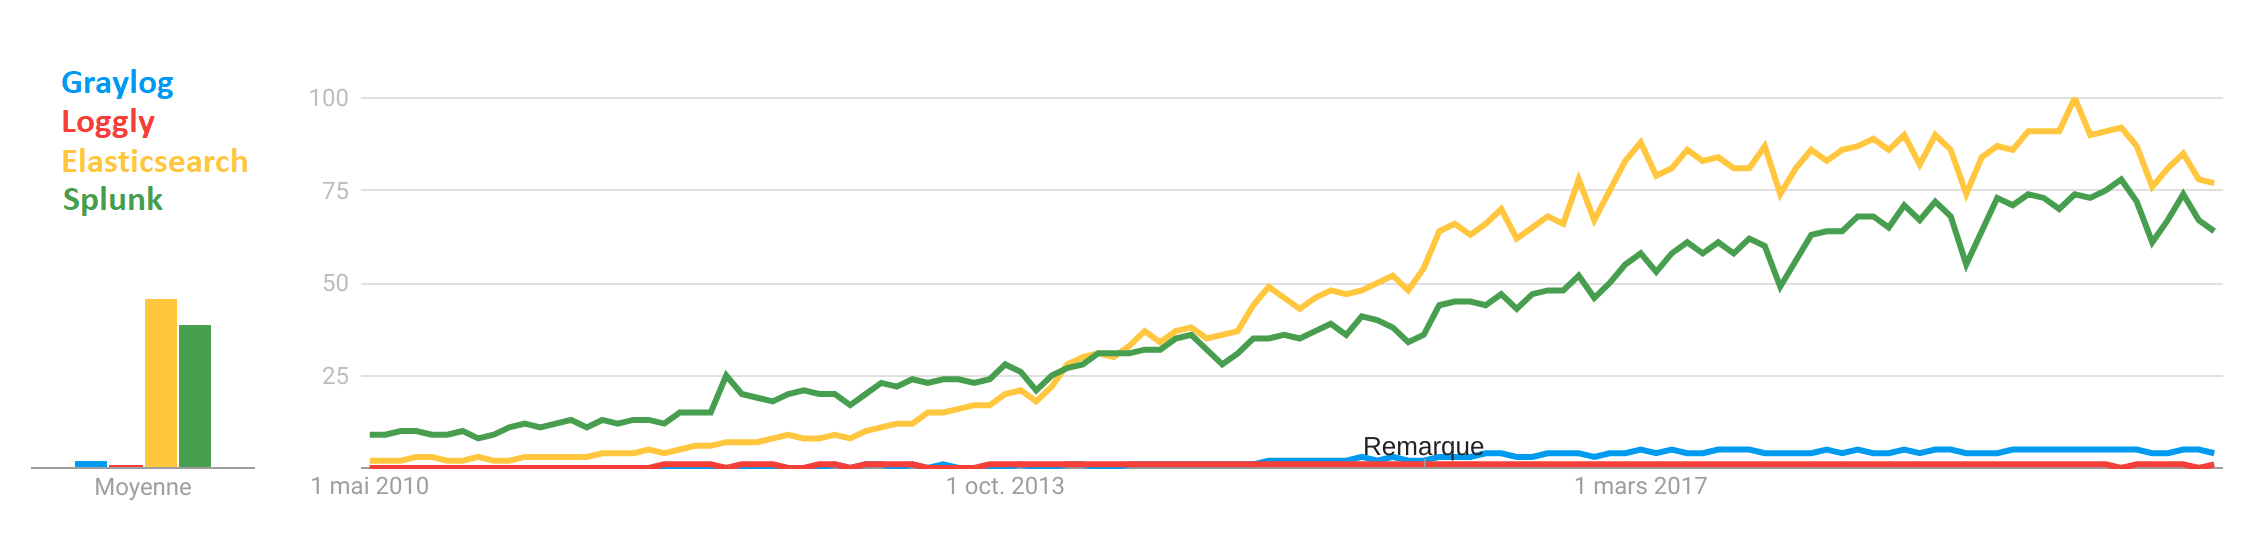
\includegraphics[width=18cm]{img/screenshots/Tendance_4.png}
    \caption{Courbes Google Trends des quatre systèmes}
    \label{f-Trends4Systemes}
\end{figure}

\begin{figure}[H]
    \centering
    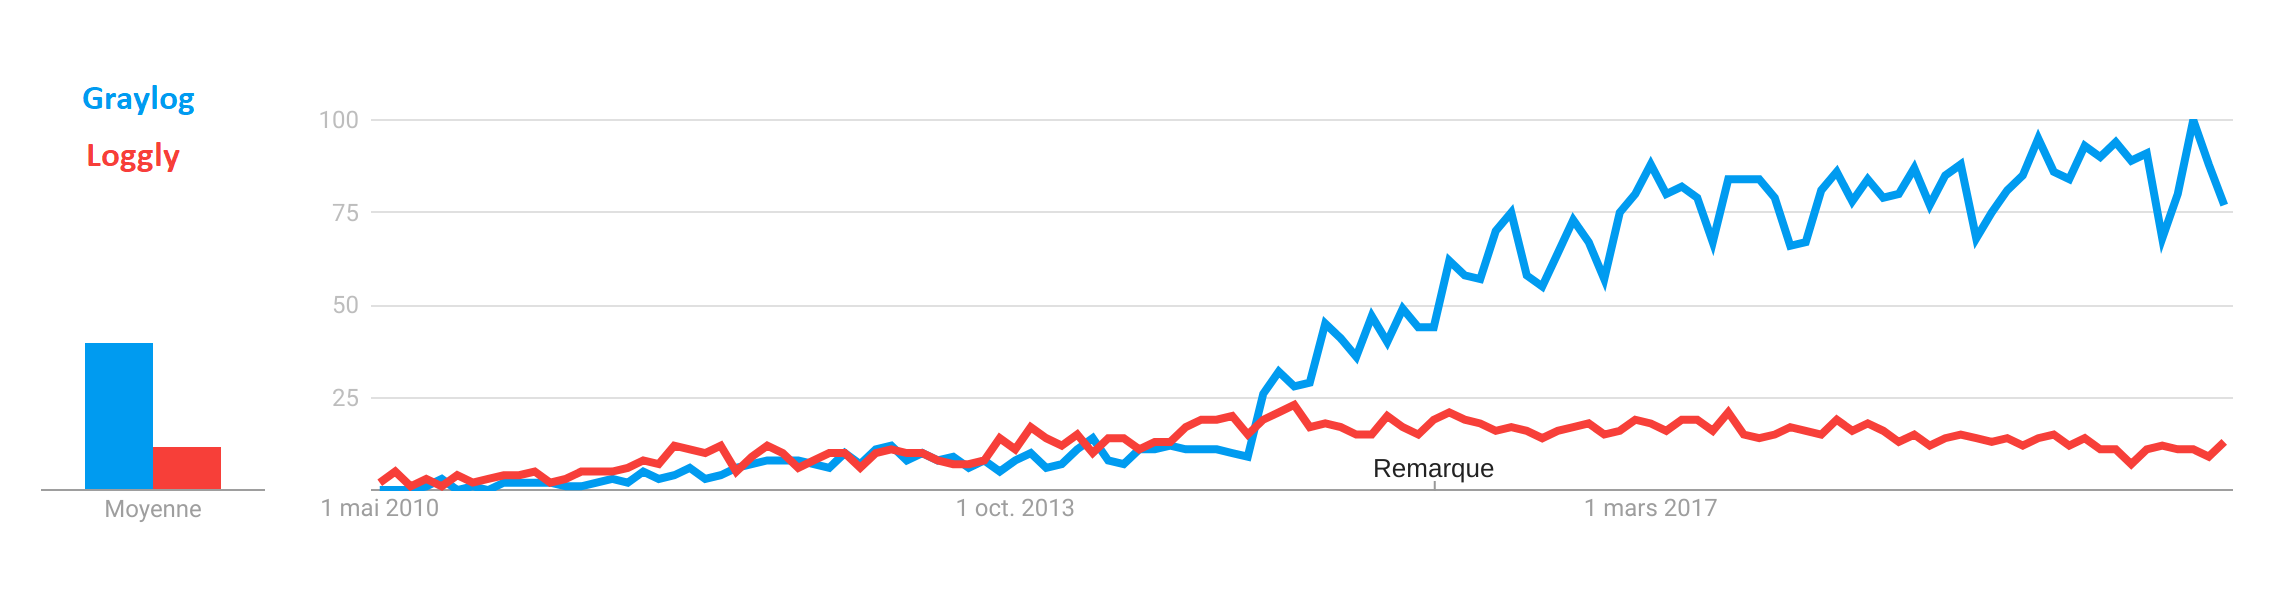
\includegraphics[width=18cm]{img/screenshots/Tendance_2.png}
    \caption{Courbes Google Trends de Graylog et Loggly}
    \label{f-Trends2Systemes}
\end{figure}

La Suite Elastic contenant 4 logiciels séparés, le choix ici a été d'inclure uniquement \og Elasticsearch \fg, car c'est la plus connue des quatre applications, et que les résultats sont meilleurs qu'avec le terme \og Elastic Stack \fg (il faut également savoir que la Suite à changé de nom en 2016, passant de \og ELK Stack \fg à \og Elastic Stack \fg, ce qui ne favorise pas la recherche dans Google Trends).

\textbf{Conclusion} \\
On distingue deux groupes dans cette analyse : Elasticsearch et Splunk d'un côté, Graylog et Loggly de l'autre. Le premier est très populaire et en croissance, alors que le deuxième n'est que peu tendance, et Loggly n'est pas en croissance. Au sein même du groupe Graylog-Loggly, on peut encore constater une grande différence, Graylog étant beaucoup plus recherché sur Google que Loggly. On peut donc affirmer que la Suite Elastic est le système le plus populaire, devant Splunk. Loin derrière vient Graylog et encore plus loin, on trouve Loggly.

\subsection{Tests réels et prise en main des logiciels}

Plusieurs tests ont été effectués afin de pouvoir effectuer une comparaison de ces systèmes. Comme la plupart de ces tests obligent une prise en main concrète des logiciels, ceux-ci ont également permis d'avoir une idée de la facilité d'utilisation, de la flexibilité ainsi que de l'utilisabilité ( \og user-friendliness \fg) des systèmes.

Voici les versions des logiciels utilisés pour effectuer ces tests :

\begin{itemize}
    \item Elastic Stack
    \subitem Elasticsearch 7.6.2
    \subitem Filebeat 7.6.2
    \subitem Logstash 7.6.2
    \subitem Kibana 7.6.2
    \item Graylog
    \subitem Graylog 3.2.4-1 (Virtual Appliance)
    \subitem Filebeat 7.6.2
    \item Splunk
    \subitem Splunk 8.0.2.1
    \subitem Splunk Universal Forwarder 8.0.2.1
    \item Loggly
    \subitem Loggly Lite (Cloud)
\end{itemize}

\subsubsection{Test de débit d'ingestion de logs} \label{sss-testDebitIngestionLogs}

Le premier test de cette comparaison consiste en un test de débit. Cela permet d'avoir une première idée de la performance des applications.

\textbf{Conditions de tests} \\
\begin{itemize}
    \item Chargement d'un fichier de logs.
    \subitem Le fichier contient 98'305 logs identiques.
    \subitem Log : 2020-02-27 09:06:24.596 INFO  o.s.s.c.ThreadPoolTaskScheduler -> Shutting down ExecutorService 'taskScheduler'
    \item On effectue un test d'ingestion simple (on stocke le log brut).
    \item On effectue un test d'ingestion avec filtre (on parse les différentes parties du log).
    \subitem Date et heure : 2020-02-27 09:06:24.596
    \subitem Niveau du log : INFO
    \subitem Classe Java : o.s.s.c.ThreadPoolTaskScheduler
    \subitem Message : Shutting down ExecutorService 'taskScheduler'
    \item Le résultat est un débit exprimé en EPS (Event Per Second), qui correspond au nombre de logs que le système aura pu ingéré en une seconde.
\end{itemize}

La table \ref{t-testIngestion} montre \textbf{les résultats} des tests d'ingestion.

\centering
\begin{table}[H]
\centering
\begin{tabular}{ |p{3cm}|p{3cm}|p{3cm}|p{3cm}|p{3cm}|  }
    \hline
    & Elastic Stack & Graylog & Splunk & Loggly \\
    \hline
    Sans filtrage & 4'898 & 14'044 & - & 46'295 (\textasteriskcentered) \\
    \hline
    Avec filtrage & 9'181 & 7'868 & 2'628 & -\\
    \hline
\end{tabular}
\caption{Résultats des tests de débit d'ingestion}
\label{t-testIngestion}
\end{table}
\justify

(*) Loggly n'acceptant que des fichiers de taille inférieure à 5 MB, le fichier à été réduit à 3'999 logs.

Splunk favorise l'extraction d'informations (parsing) après avoir stocké les logs dans le système. Il est alors compliqué d'ajouter un filtrage avant le stockage et ça n'a donc pas été réalisé. Par contre, Splunk effectue automatiquement une extraction de la date des logs. Son débit à donc été classé dans la catégorie \og avec filtrage \fg.
Loggly ayant été écarté assez tôt de l'évaluation, la partie \og avec filtrage \fg n'a pas été testée. \\

\textbf{Conclusion} \\
Sans filtrage, on constate que Graylog possède un débit supérieur à Elastic Stack. Loggly n'acceptant pas des fichiers de grande taille, il est difficilement comparable. Avec filtrage, étonnemment, la Suite Elastic gagne en débit. Elle possède donc un meilleur débit que Graylog et Splunk.
Après ce test, outre les résultats comptables, il se dessine surtout une tendance vers Graylog et Elastic Stack, car ces deux systèmes sont plus \og ouvert \fg que les autres. Il n'y a pas eu de difficultés particulières lors de l'utilisation, pas de contraintes comme la taille du fichier ou encore le moment du filtrage au sein du pipeline.

\subsubsection{Test d'ingestion d'une grande quantité de logs}

Ce test a pour but de mettre en évidence les limites de certains systèmes lors de l'ingestion de gros fichier de logs. Il permet également d'avoir une brève vue sur la constance du débit mesuré lors du test précédent.

\textbf{Conditions de tests} \\
\begin{itemize}
    \item Chargement d'un fichier de logs.
    \subitem Le fichier contient 999'999 logs identiques.
    \subitem Log : 2020-02-27 09:06:24.596 INFO o.s.s.c.ThreadPoolTaskScheduler -> Shutting down ExecutorService ’taskScheduler’
    \item On n'effectue aucun traitement sur le log.
    \item Le résultat est soit une limite supérieure, soit \og > 1'000'000 \fg
\end{itemize}

La table \ref{t-testGrandeIngestion} montre \textbf{les résultats} du test d'ingestion d'une grande quantité de logs.

\centering
\begin{table}[H]
\centering
\begin{tabular}{ |p{3cm}|p{3cm}|p{3cm}|p{3cm}|p{3cm}|  }
    \hline
    Elastic Stack & Graylog & Splunk & Loggly \\
    \hline
    > 1'000'000 & > 1'000'000 & > 1'000'000 & \textasciitilde 4'000 (5 MB) \\
    \hline
\end{tabular}
\caption{Résultats des tests d'ingestion de grande quantité de logs}
\label{t-testGrandeIngestion}
\end{table}
\justify

\textbf{Conclusion} \\
Ce test permet simplement de montrer que les systèmes travaillant avec un agent, soit selon la méthode PUSH, n'ont pas de problème de taille de fichier, car l'agent lit et envoie les logs au fur et à mesure. Loggly est le seul ici utilisant la méthode PULL. Au niveau des débits, par rapport au test d'ingestion du paragraphe \ref{sss-testDebitIngestionLogs}, ceux d'Elastic Stack et de Graylog ont été divisés par 2, alors que celui de Splunk est resté stable. Pour Loggly, il n'y a pas eu de différence, étant donné qu'il est limité en taille de fichier.


\subsubsection{Test de consommation CPU}

Ce test-ci a pour but de pouvoir comparer les systèmes de gestion de logs Elastic Stack et Graylog en terme de performance.

\textbf{Conditions de test} \\
\begin{itemize}
    \item Chargement du même fichier de log que pour le test de débit du paragraphe \ref{sss-testDebitIngestionLogs}.
    \item L'utilisation du CPU sera réduite au minimum hors système à tester.
    \item Ordinateur de test : ASUS UX360UAK
    \item Processeur : Intel Core i7-7500U CPU @ 2.70GHz x 4
    \item Lors de la réception, l'agent Filebeat se situera sur une autre machine.
\end{itemize}

\textbf{Résultats} \\
La figure \ref{f-ElasticCPU} montre la consommation CPU et l'historique du trafic réseau lors de la réception des logs pour le système Elastic Stack. La figure \ref{f-GraylogCPU} montre les mêmes informations, mais pour le système Graylog. Enfin, la figure \ref{f-FilebeatCPU} montre ces informations-ci avec l'agent Filebeat envoyant des logs.

\begin{figure}[H]
    \centering
    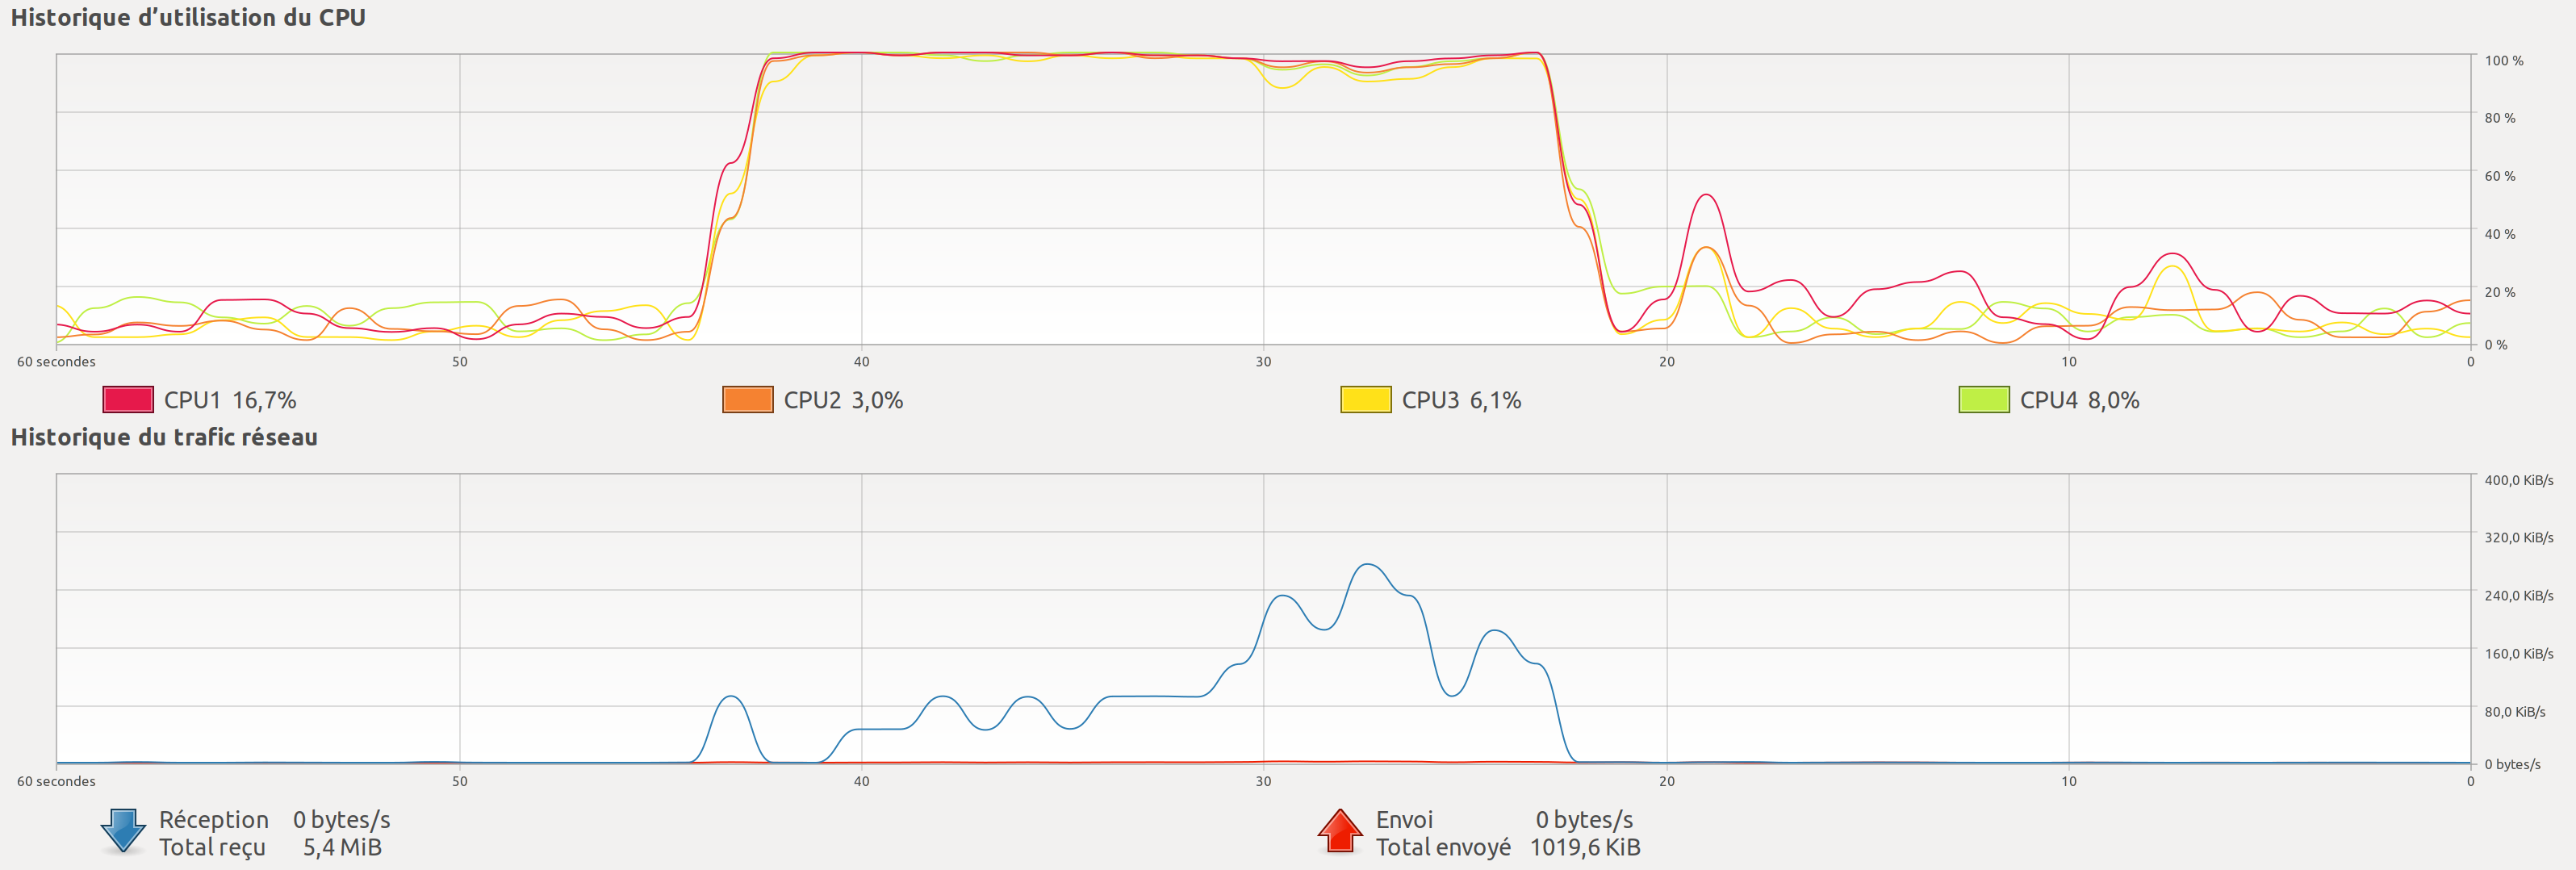
\includegraphics[width=18cm]{img/screenshots/Elastic_CPU_MEM_Receive_modified.png}
    \caption{Consommation CPU Elastic Stack}
    \label{f-ElasticCPU}
\end{figure}

\begin{figure}[H]
    \centering
    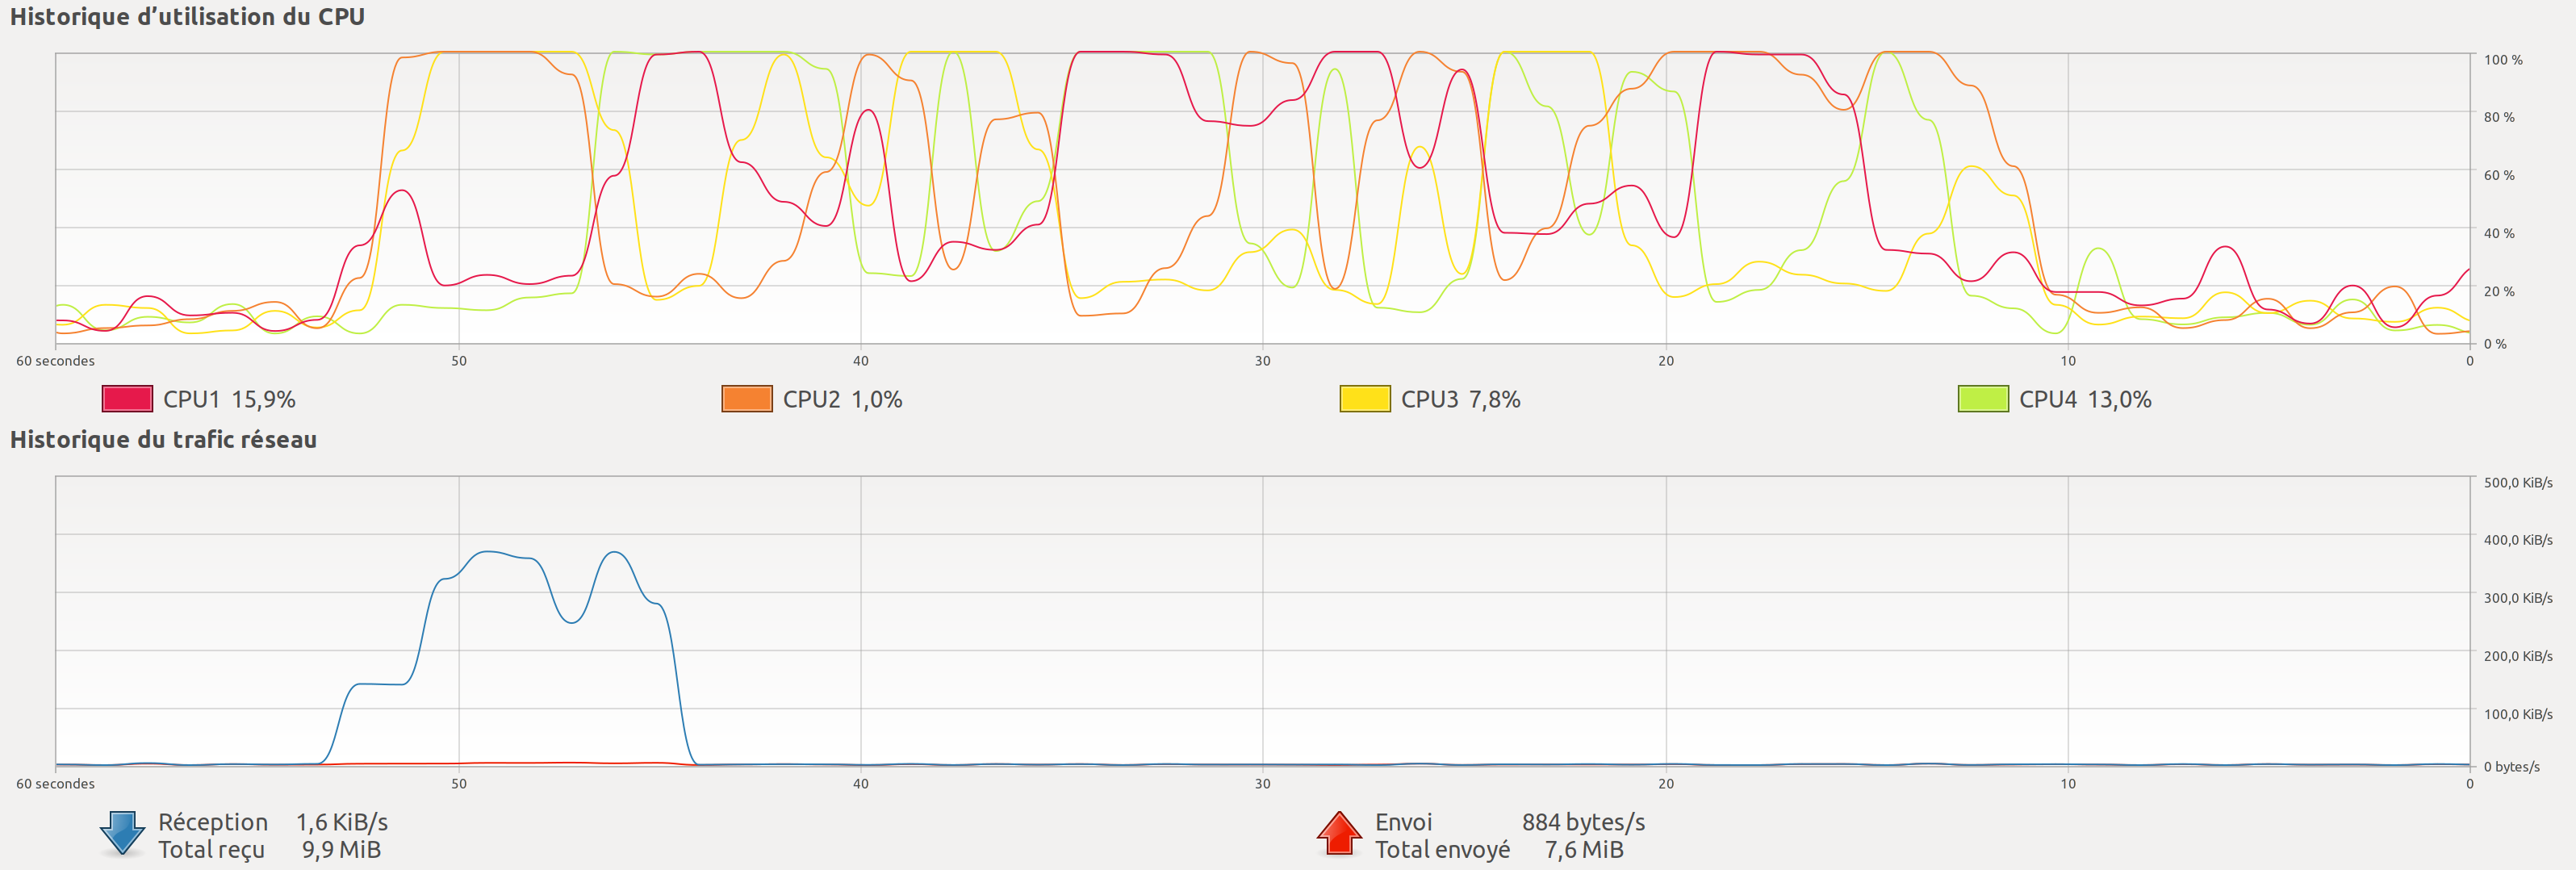
\includegraphics[width=18cm]{img/screenshots/Graylog_CPU_MEM_Receive_modified.png}
    \caption{Consommation CPU Graylog}
    \label{f-GraylogCPU}
\end{figure}

\begin{figure}[H]
    \centering
    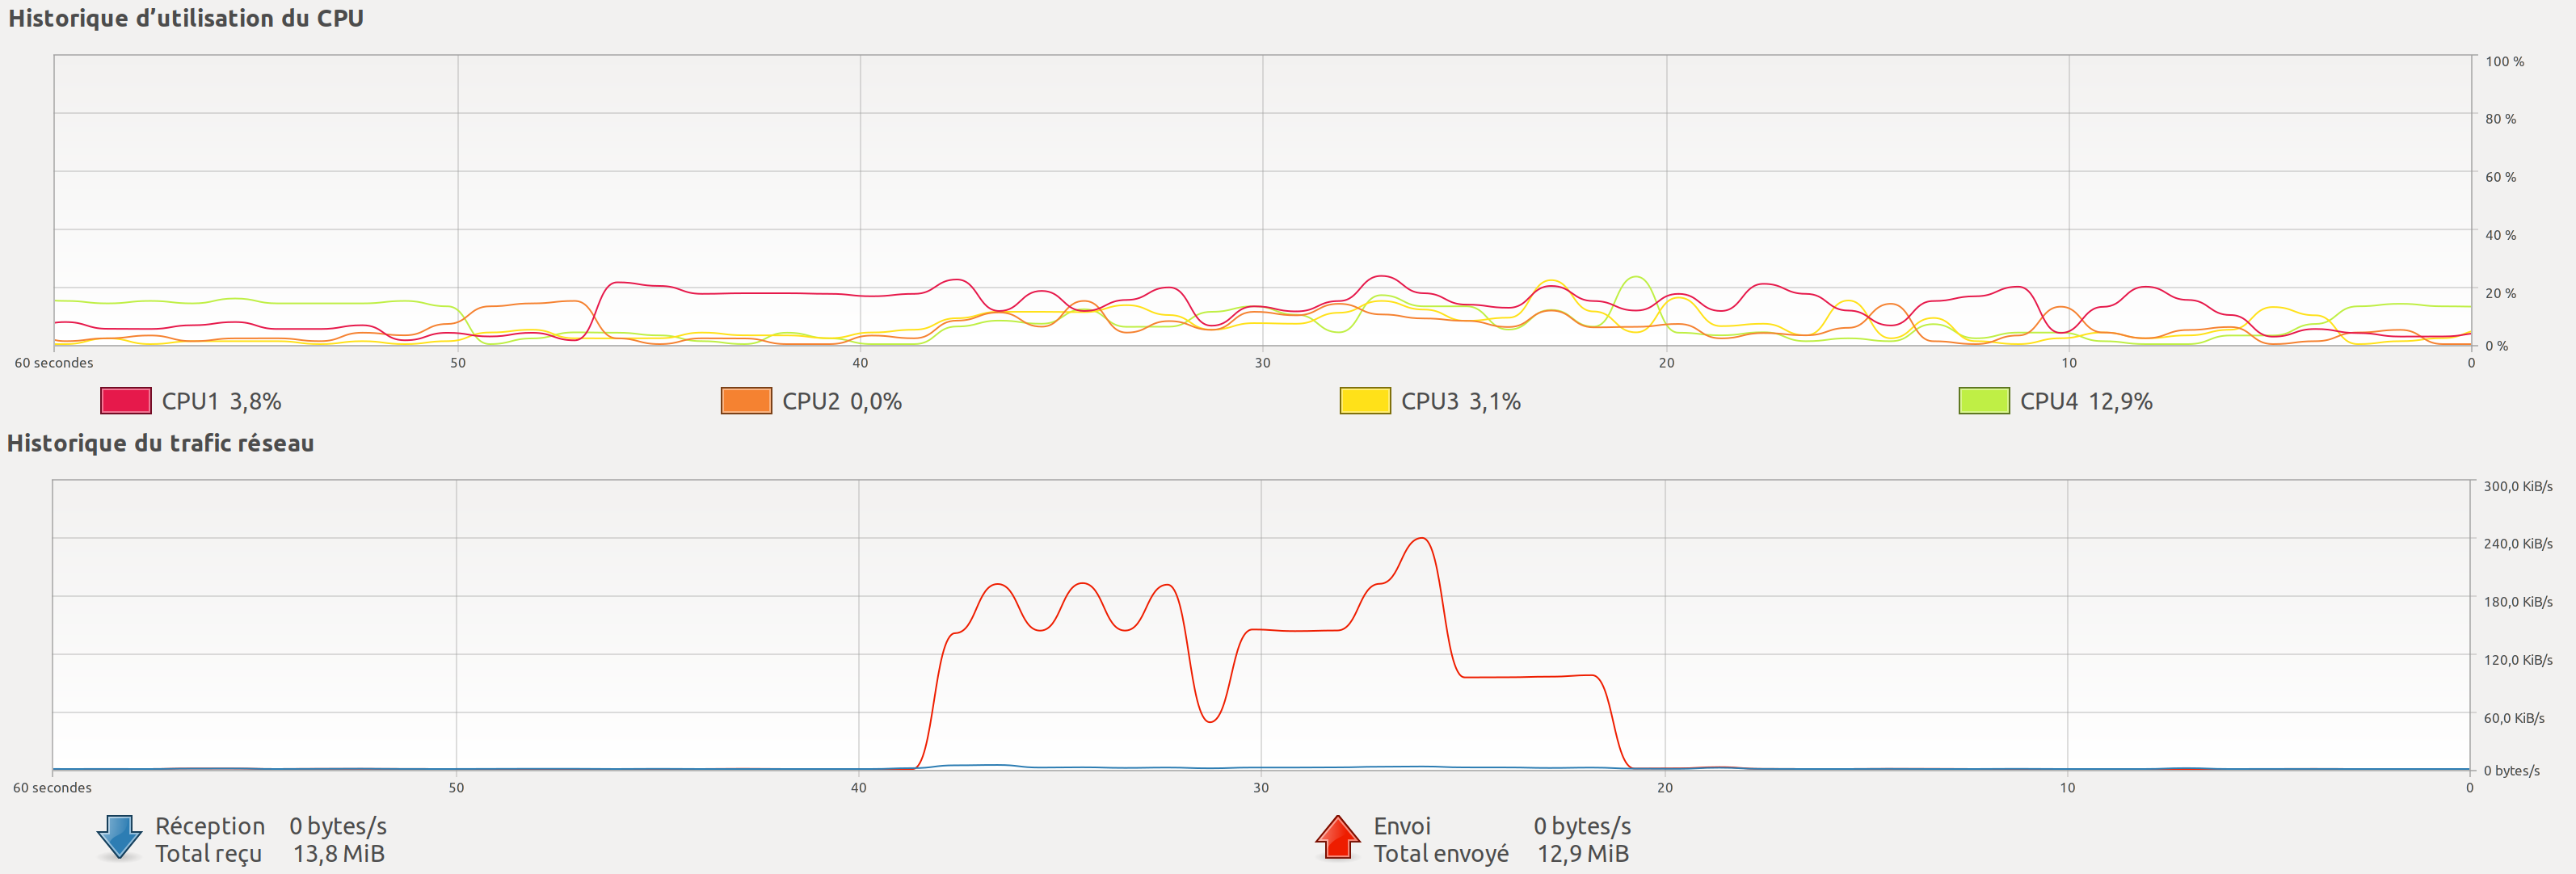
\includegraphics[width=18cm]{img/screenshots/Filebeat_send_modified.png}
    \caption{Consommation CPU Filebeat}
    \label{f-FilebeatCPU}
\end{figure}

\textbf{Conclusion} \\
Premièrement, on constate que l'agent Filebeat est un agent très léger puisque son action ne se fait quasiment pas ressentir sur le taux d'utilisation du CPU. Pour ce qui est du taux d'utilisation CPU par la Suite Elastic, on remarque que lors de la réception et le stockage des logs, tous les CPUs tournaient à 100\% de leur capacité, et la charge dure environ 25 secondes. Pour Graylog, les CPUs ne sont pas autant sollicité, ou du moins pas tous en même temps. Ils varient entre 20\% et 100\% et la distribution est plutôt égale entre les CPUs. On peut donc estimer un taux d'utilisation moyen à 60-70\%. La charge dure cette fois-ci environ 45 sec. À noter que Graylog ingère les logs en env. 7 secondes, puis travaille encore pendant env. 35 secondes, alors que la Suite Elastic fait tout en même temps. On peut constater ceci grâce à la courbe de l'historique du trafic réseau.

\subsection{Conclusion de la comparaison des outils}
\subsubsection{Analyse théorique des systèmes}
Au niveau fonctionnel, les quatre systèmes de gestion de logs ne se différencient pas énormément. Ils suivent à peu près tous le même schéma et permettent tous de faire les mêmes actions (reporting, alerting, analyse, etc.). Loggly est légèrement différent dans le sens où son approche de collecte de log par défaut est maximaliste (approche PULL). Il met en effet un endpoint à disposition, sur lequel on peut envoyer des données. Il s'agit la d'une différence mineure car bien que les autres systèmes privilégient et facilitent l'approche minimaliste, il est également possible de configurer un endpoint semblable pour les systèmes Elastic Stack, Graylog et Splunk. \newline
Pour ce qui est du non-fonctionnel, il y a quelques points où les systèmes se démarquent. Premièrement, Loggly de SolarWinds est uniquement disponible dans une version Cloud. La Suite Elastic et Splunk sont eux disponibles tant dans une version Cloud que dans une version sur site. Graylog lui est uniquement disponible dans une version locale. Il y a également l'architecture des systèmes. La Suite Elastic est formée de 3 applications indépendantes, et en utilise une 4\ts{ème} pour l'agent Beat. Graylog est composé d'un système, et utilise des agents ne lui appartenant pas, comme Beat. Splunk suit la même architecture que Graylog, mais possède son propre agent, le Splunk Forwarder. Et Loggly est une infrastructure cloud sans agent. \newline
Reste la comparaison de la popularité des applications. Celle-ci a montré une nette avance pour Splunk et Elastic Stack, devant Graylog, puis Loggly qui est vraiment peu populaire. \newline
La table \ref{t-resumeAnalyseTheorique} résume ces différentes propriétés.

\begin{table}[H]
\centering
\begin{tabular}{ |m{2.9cm}|m{4cm}|m{2.9cm}|m{2.9cm}|m{3.2cm}|  }
    \hline
     & \textbf{Elastic Stack} & \textbf{Splunk} & \textbf{Graylog} & \textbf{Loggly} \\
    \hline
    Fonctionnalités & \multicolumn{4}{c|}{Reporting, alerting, analyse, etc.}\\
    \hline
    Cloud / On-Prem & \multicolumn{2}{c|}{Cloud ou Sur site} & Sur site & Cloud \\
    \hline
    Architecture  & Suite (3 outils + agent) & \multicolumn{2}{c|}{Un système + agent} & Cloud (sans agent) \\ 
    \hline
    Popularité & \multicolumn{2}{c|}{Très populaire} & Peu populaire & Très peu populaire \\
    \hline
\end{tabular}
\caption{Résumé de la conclusion de l'analyse théorique}
\label{t-resumeAnalyseTheorique}
\end{table}

Globalement, l'analyse théorique des systèmes de gestion de logs ne permet pas de faire un choix concret sur un système ou un autre pour la réalisation d'une solution destinée au système GridEye. Elle permettrait tout au plus de se détacher de Loggly, qui n'est vraiment pas recommandable du point de vue de sa courbe de tendance.
\subsubsection{Analyse pratique des systèmes}
Le but des tests réels était de pouvoir confronter les systèmes de gestion de log au niveau de leur performance, et également de réaliser une prise en main des différents logiciels, avec tout ce que cela implique (installation, configuration, etc.). Cette deuxième partie avait également pour but d'évaluer l'utilisabilité des divers systèmes.
Au niveau des performances, on a pu voir que les systèmes Graylog et Elastic Stack se distinguaient légèrement avec un meilleur débit d'ingestion. Que tous les systèmes, excepté Loggly, pouvaient, grâce à leur approche minimaliste, recevoir des grandes quantités de logs.\\
À ce point-ci de la comparaison, un premier bilan de l'\og user-friendliness \fg des systèmes à également pu être tiré :
\begin{itemize}
    \item SolarWinds Loggly est relativement simple d'utilisation. Sa caractéristique Cloud facilite également l'installation (il n'y en a pas, il suffit de se créer un compte et nous recevons un lien vers notre version d'essai).
    \item Graylog est un système ayant une interface plutôt complète et efficace. L'interface graphique permet directement de configurer le système de manière simple (elle permet d'ajouter des règles d'extraction d'informations dans les logs, de configurer les entrées ouvertes aux agents, etc.).
    \item Elastic Stack est une \og suite \fg de logiciels, ce qui la rend très ouverte. On peut en effet choisir d'utiliser ses softwares de base, mais également utiliser d'autres applications. Par exemple, on peu prendre un agent de la famille Beat, mais on pourrait aussi choisir un agent Prometheus. Chaque logiciel est configurable via des fichiers de configuration. On peut également choisir d'utiliser les 4 logiciels, ou pas. Par exemple enlever Logstash si l'on a pas besoin de ces filtres. Cette ouverture le rend agréable à utiliser.
    \item Splunk est comparable à Graylog et Elastic Stack dans tous les tests, mais l'expérience utilisateur est de son côté moins bonne. Le système est plus une sorte de \og boîte noire \fg dans laquelle il n'est pas possible de tout configurer. L'extraction des informations des logs n'a par exemple pas pu avoir lieu avant l'indexage, car le système est prévu pour le faire après.
\end{itemize}
Avec ces premiers tests, nous avons déjà pu écarter la solution SolarWinds Loggly, qui ne correspondait pas aux attentes et dont les contraintes liées au Cloud ne sont pas souhaitées. Splunk n'est également pas recommandé à cause de son manque d'ouverture.
Ensuite, il y a encore eu le test d'utilisation du CPU entre la Suite Elastic et Graylog. Avec celui-ci, on pourrait donner un très léger avantage à Graylog.

\subsubsection{Recommandation}
En conclusion, il est difficile de faire un choix entre les deux systèmes Graylog et la Suite Elastic. Mais de part sa très grande popularité, amenant son lot de réponse dans les forums et autres articles permettant d'accélérer le développement d'un logiciel, ainsi que de son caractère très ouvert lié à son \og architecture suite \fg, la \textbf{Suite Elastic} est le meilleur choix dans l'optique de mise en place d'une solution de gestion de logs pour l'infrastructure GridEye.

\newpage

\section{Implémentation du cas d'utilisation}

Un cas d'utilisation à implémenter à été fourni par DEPsys et demande les éléments suivants :

Le système générant les logs sera composé d'une base de donnée PostgreSQL \cite{noauthor_postgresql_nodate} et d'une application Java \cite{noauthor_java_nodate} simulant différents comportements, comme une surcharge du CPU, de la RAM ou autres problèmes.

Le système Elastic Stack devra mesurer plusieurs métriques :
\begin{itemize}
    \item Redémarrage de conteneur.
    \item Taux d'utilisation de la mémoire.
    \item Occupation de la base de données (PostgreSQL).
    \item Taux d'utilisation du CPU.
    \item Les crashs Java
    \item Et éventuellement d'autres métriques comme les logs de l'application Java.
\end{itemize}

Plusieurs instances peuvent être lancées en même temps, ce qui permet de simuler au mieux la réalité (il y a plusieurs \og field device \fg).

Il doit être possible de savoir si le système est fonctionnel, et à quel point.

Pour répondre à toutes ces demandes, on va commencer par installer et configurer tous les outils de la Suite Elastic qui seront utilisés, et ce avec Docker \cite{noauthor_empowering_nodate}.
Ensuite, nous allons créer des visualisations avec Kibana. Elles permettront de connaître l'état du système en temps réel, et de retrouver la cause des problèmes, s'il y en a.

\subsection{La Suite Elastic avec Docker}
Afin de faciliter les étapes d'installation, de configuration et de lancement de la Suite Elastic, une version \og dockerisée \fg des différents logiciels est une solution idéale. Elle permet également d'uniformiser ces étapes-ci. En effet, l'installation des applications de la Suite Elastic sans conteneur fonctionnera de la même manière sur des systèmes Ubuntu, voire Linux, mais sera différente sur un système d'exploitation Microsoft Windows par exemple. L'utilisation de conteneurs comble ces problèmes.

L'installation à été séparée en deux, car deux machines sont nécessaires pour simuler l'interface GridEye : une machine serveur, recevant les logs, et une machine client, envoyant les logs.
\subsubsection{Machine hôte de \og ELK \fg}
Par \og ELK \fg, qui est l'ancien nom de la Suite Elastic, on parle des trois outils Logstash, Elasticsearch et Kibana. C'est la machine qui ne sera pas sur le terrain et qui permettra l'agrégation, le stockage et l'analyse des logs, entre autres.
La figure \ref{f-dockerTopology} montre un schéma de la topologie Docker prévue permettant de faire fonctionner ensemble les différents outils de la Suite Elastic.
\begin{figure}[H]
    \centering
    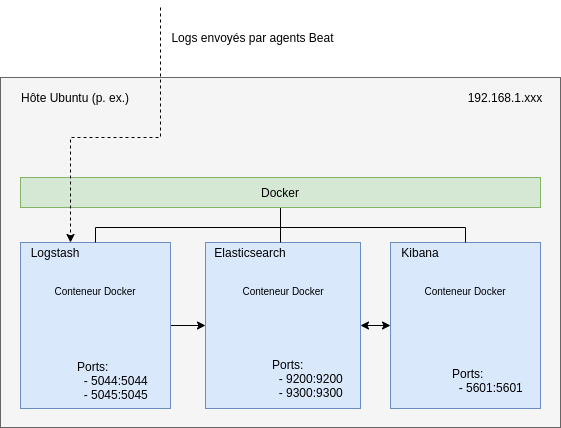
\includegraphics[width=11cm]{img/ElasticStack_docker_topology.png}
    \caption{Architecture de l'implémentation du use-case - côté \og ELK \fg}
    \label{f-dockerTopology}
\end{figure}

Comme il y a plusieurs conteneurs Docker devant être créés, nous allons utiliser l'outil \verb,docker-compose, \cite{noauthor_overview_2020} qui permet de gérer et d'orchestrer de multiples conteneurs. Nous aurons trois images à aller télécharger : Logstash, Elasticsearch et Kibana. L'agent Beat se situant sur un ordinateur distant, il n'est pas inclus dans cette topologie. La figure \ref{f-treeDocker} montre l'arborescence des dossiers et fichiers nécessaires.
\begin{figure}[H]
    \centering
    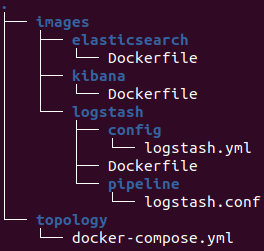
\includegraphics[width=7cm]{img/screenshots/tree_docker.png}
    \caption{Arborescence de la topologie Docker - côté ELK}
    \label{f-treeDocker}
\end{figure}
Les \verb,Dockerfile, des images Elasticsearch et Kibana sont très simples, ils vont simplement télécharger les images correspondantes depuis le \verb,Elastic Docker registry,.\\
\verb,Dockerfile, d'Elasticsearch :
\begin{lstlisting}
FROM docker.elastic.co/elasticsearch/elasticsearch:7.6.2
\end{lstlisting}
\verb,Dockerfile, de Kibana :
\begin{lstlisting}
FROM docker.elastic.co/kibana/kibana:7.6.2
\end{lstlisting}

Pour l'image de Logstash, il y aura deux fichiers de configurations. Un pour le \og pipeline \fg, qui contiendra les configurations d'entrées, filtres et sorties, et un pour les paramètres de l'outil. \\
Fichier de configuration des paramètres (\verb,logstash.yml,) :
\begin{lstlisting}
http.host: "0.0.0.0"
xpack.monitoring.elasticsearch.hosts: [ "http://elasticsearch:9200" ]
\end{lstlisting}
La configuration du pipeline se fait dans un fichier \verb,.conf, nommé \verb,logstash.conf, et qui ira se copier à l'adresse \verb,/usr/share/logstash/pipeline/, du système de fichier du conteneur. Le fichier peut avoir un nom différent, tant qu'il porte l'extension \verb,.conf,.

Le fichier de configuration de Logstash est divisé en trois parties :
\begin{enumerate}
    \item input
    \subitem Cette première partie permet de configurer l'arrivée des logs. Il est possible d'y configurer un agent Beat, ce qui nous concernera ici, mais également la lecture directe d'un fichier, ou de beaucoup d'autres sources, comme Twitter, JDBC, etc.
    \item filter
    \subitem La partie filtre permet quant à elle de parser les logs. Il existe là aussi beaucoup de filtres différents. Nous utiliserons une structure \verb,grok, qui permet de parser des événements non structurés.
    \item output
    \subitem La sortie sert à choisir où Logstash enverra ses logs traités. En général, il s'agit d'Elasticsearch.
\end{enumerate}

Pour la configuration de l'entrée, nous allons simplement écouter deux agents Beat, chacun sur un port donné. Nous allons également ajouté un tag \verb,filebeat, qui sera utilisé pour la partie \og filtre \fg.
\begin{lstlisting}[language=bash]
input {
    beats {
        port => 5044
        tags => ["filebeat"]
    }

    beats {
        port => 5045
    }
}
\end{lstlisting}
En ce qui concerne le filtre, nous allons parser les logs envoyés par le logiciel de simulation de GridEye. Le format des logs est défini par la ligne suivante :
\begin{lstlisting}
%d{yyyy-MM-dd HH:mm:ss.SSS} %-5level %logger{100} -> %msg%n
\end{lstlisting}
Le site \verb,grokconstructor, \cite{noauthor_test_nodate} permet de créer des \verb,grok pattern, de façon incrémentale. Il suffit de lui donner quelques lignes de logs générés par notre application et de le configurer. Il va ensuite nous proposer des motifs qu'il détecte dans les lignes de logs données. Voici le résultats après lui avoir donné quelques lignes générés par le simulateur :
\begin{lstlisting}
\A%{TIMESTAMP_ISO8601}%{SPACE}%{LOGLEVEL}%{SPACE}%{JAVACLASS} -> %{JAVALOGMESSAGE}
\end{lstlisting}
À savoir que le tout premier champ, qui a été défini comme un \verb,TIMESTAMP_ISO8601,, n'en est pas vraiment un \cite{noauthor_iso_2020}. Mais c'est le motif qui correspond le mieux à notre format de date-heure.
Il reste à définir des labels décrivant les différents motifs. Ces labels seront utilisés par Kibana.
\begin{lstlisting}
\A%{TIMESTAMP_ISO8601:date_hour}%{SPACE}%{LOGLEVEL:log_level}%{SPACE}%{JAVACLASS:class} -> %{JAVALOGMESSAGE:message}
\end{lstlisting}
Comme ce \verb,grok pattern, permet de parser uniquement nos logs applicatifs, il faut ajouter une condition, qui indique que si les logs viennent d'ailleurs (p. ex. de la base de données PostgreSQL), ils ne doivent pas être parsés par ce filtre. Nous allons utiliser le tag \verb,filebeat,.
\begin{lstlisting}[language=bash]
filter {
    if ("filebeat" in [tags]) {
	grok { 
	    match => {"message" => "%{TIMESTAMP_ISO8601:date_hour}%{SPACE}%{LOGLEVEL:log_level}%{SPACE}%{JAVACLASS:class} -> %{JAVALOGMESSAGE:log_message}"}
	}
}
\end{lstlisting}
Pour finir, la partie sortie défini uniquement l'adresse et le port de notre instance Elasticsearch.
\begin{lstlisting}[language=bash]
output {
    elasticsearch {
        hosts => ["elasticsearch:9200"]
    }
}
\end{lstlisting}
Le fichier complet \verb,logstash.conf, est disponible dans l'annexe \ref{appendix:logstashConf}.

Le \verb,Dockerfile, de Logstash télécharge l'image, puis ajoute les fichiers de configuration au système de fichier du conteneur.
\begin{lstlisting}
FROM docker.elastic.co/logstash/logstash:7.6.2
RUN rm -f /usr/share/logstash/pipeline/logstash.conf
ADD pipeline/ /usr/share/logstash/pipeline/
ADD config/ /usr/share/logstash/config/
\end{lstlisting}

Pour finir, le fichier \verb,docker-compose.yml, organise toute la topologie. Il lancera d'abord Elasticsearch, puis Kibana, et enfin Logstash. Les ports par défaut des différents logiciels seront exposés, afin d'être accessible depuis l'extérieur. Ceci est nécessaire pour permettre la communication entre les différents conteneurs.
\lstinputlisting{files/docker-compose_impl_usecase.yml}
Un répertoire GitHub \cite{jael24_jael24tb_elasticstack_2020} contient toute l'architecture décrite.

Pour lancer le déploiement de la Suite Elastic, il suffit de lancer la commande \verb,docker-compose up --build -d, à l'endroit où se situe le fichier \verb,docker-compose.yml,. Dans ce cas-ci, le dossier \verb,topology,.
Pour tester si tout le déploiement s'est bien déroulé, une vérification d'Elasticsearch et de Kibana s'impose. 

Premièrement, avec un navigateur, la visite de l'adresse \verb,http://localhost:9200/_cat/indices, permet de constater le fonctionnement d'Elasticsearch et de Logstash. En effet, si tout se passe bien, on devrait voir les différents indices contenu dans la base de données, dont un s'appelant \verb,logstash...,. La figure \ref{f-elsearchIndices} montre cette configuration réussie.

\begin{figure}[H]
    \centering
    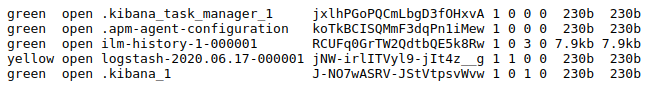
\includegraphics[width=11cm]{img/screenshots/elasticsearchLogstashOk.png}
    \caption{Indices contenus dans la base de données Elasticsearch, avec Logstash}
    \label{f-elsearchIndices}
\end{figure}

Deuxièmement, toujours dans un navigateur, à l'adresse \verb,localhost:5601,, il devrait y avoir l'application Kibana qui est lancée. La figure \ref{f-kibanaInstalled} montre ceci.

\begin{figure}[H]
    \centering
    
\includegraphics[width=11cm]{img/screenshots/kibana_installed.png}
    \caption{Application Kibana lancée}
    \label{f-kibanaInstalled}
\end{figure}

\subsubsection{Machine \og terrain \fg} \label{ss-machineTerrain}
La machine sur le terrain contiendra les agents Beat nécessaires, ainsi que les programmes et applications générant les logs. Il y aura également une base de données contenant des données arbitraires. La figure \ref{f-dockerFieldTopology} montre l'architecture définie pour l'implémentation du use-case sur la machine \og terrain \fg.

\begin{figure}[H]
    \centering
    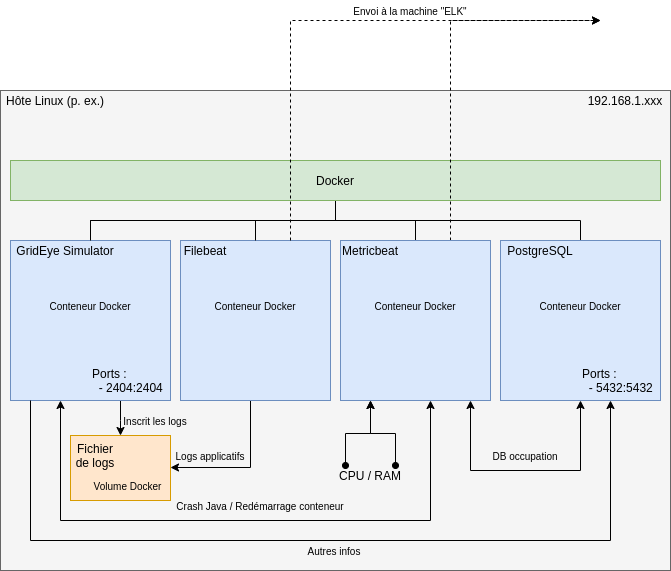
\includegraphics[width=11cm]{img/Beat_docker_topology.png}
    \caption{Architecture de l'implémentation du use-case - côté terrain}
    \label{f-dockerFieldTopology}
\end{figure}

Il y aura donc le simulateur GridEye générant les logs, un agent Filebeat qui va lire les logs applicatifs et les envoyer à la Suite Elastic (les logs seront partagés entre les deux conteneurs via un Volume Docker, qui sera lié à un chemin sur la machine hôte), un agent Metricbeat qui va surveiller le système hôte ainsi que la base de données. L'agent Metricbeat contiendra également le module de monitoring de Docker, qui nécessite un Volume Docker permettant l'accès au \og Daemon Docker \fg. Il enverra finalement les logs vers la machine hôte ELK. Pour finir, il y aura la base de donnée, qui sera un système de gestion de bases de données relationnelle (SGBDR) PostgreSQL.
Comme pour la machine contenant les outils \og ELK \fg, nous allons travailler avec un \verb,docker-compose,, qui permettra d'orchestrer tous les conteneurs. La figure \ref{f-treeDockerField} montre l'arborescence des dossiers et fichiers contenant les images Docker ainsi que le fichier \verb,docker-compose.yml,. Cette arborescence reprend les mêmes bases que celle du côté ELK.

\begin{figure}[H]
    \centering
    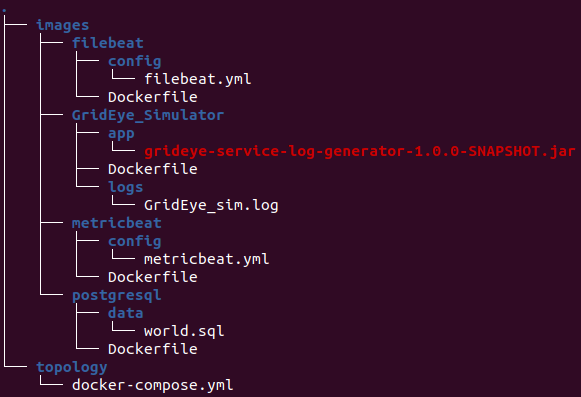
\includegraphics[width=11cm]{img/screenshots/tree_docker_field.png}
    \caption{Arborescence de la topologie Docker - côté terrain}
    \label{f-treeDockerField}
\end{figure}

Les images \verb,filebeat, et \verb,metricbeat, ont la même structure. Un \verb,Dockerfile, qui télécharge l'image correspondante depuis le \verb,Elastic Docker registry,, puis qui copie le fichier de configuration de l'agent, respectivement \verb,filebeat.yml,, et \verb,metricbeat.yml,.

\verb,Dockerfile, de filebeat
\begin{lstlisting}
FROM docker.elastic.co/beats/filebeat:7.6.2
COPY config/filebeat.yml /usr/share/filebeat/filebeat.yml
USER root
RUN chown root:filebeat /usr/share/filebeat/filebeat.yml
USER filebeat
\end{lstlisting}

\verb,Dockerfile, de metricbeat
\begin{lstlisting}
FROM docker.elastic.co/beats/metricbeat:7.6.2
COPY config/metricbeat.yml /usr/share/metricbeat/metricbeat.yml
USER root
RUN chown root:metricbeat /usr/share/metricbeat/metricbeat.yml
\end{lstlisting}

La configuration de Filebeat se fait dans un fichier \verb,YAML,, qui se nomme \verb,filebeat.yml,, et qui sera copié dans le répertoire \verb,/usr/share/filebeat/, du conteneur. Il y a un grand nombre de paramètres de configuration disponibles. Dans le cas de notre utilisation, il n'y a que deux paramètres à configurer : l'entrée à lire ainsi que la sortie.
Pour l'entrée, il suffit de faire pointer le paramètre vers le fichier dans lequel le simulateur GridEye écrit ses logs.
\begin{lstlisting}[language=bash]
filebeat.inputs:
  - type: log
    enabled: true
    paths:
            - /usr/share/filebeat/logs/GridEye_sim.log
\end{lstlisting}
Pour la sortie, on va informer l'adresse de l'instance de Logstash configuré plus tôt.
\begin{lstlisting}[language=bash]
output.logstash:
  hosts: ["<IP>:5044"]
\end{lstlisting}
Il faut remplacer \verb,<IP>, par l'adresse IP de la machine hébergeant Logstash.

Pour Metricbeat, la configuration est similaire. Elle se fait également dans un fichier \verb,YAML,, qui se nomme \verb,metricbeat.yml,, et qui sera copié dans le répertoire \verb,/usr/share/metricbeat/, du conteneur.

Il y a deux paramètres à configurer : les modules de métriques à surveiller, ainsi que la sortie.

Pour les modules de métriques, nous allons utiliser \verb,system,, qui permettra d'obtenir les informations sur la mémoire et le CPU. Le module \verb,postgresql, nous permettra lui d'obtenir les métriques de la base de données. Et pour finir, le module \verb,docker, enverra lui les métriques concernant les redémarrages de conteneur, et les crashs Java.

La configuration de sortie est la même que pour Filebeat, mais avec le port 5045.

Les fichiers de configuration des deux agents sont disponibles aux annexes \ref{appendix:filebeatConfDockerUC} (filebeat) et \ref{appendix:metricbeatConfDockerUC} (metricbeat).

L'image du simulateur de la plateforme GridEye contient elle un \verb,Dockerfile, qui va lancer une application Java depuis un fichier \verb,jar,. Cette manière de lancer une application Java dockerisée est la plus simple pour ce cas présent (le fichier compilé ne change jamais car il n'y a pas de mise à jour du programme). Il y a également un dossiers \verb,logs, qui contiendra le fichier de log et sera donc la base du Volume Docker partagé avec l'agent filebeat. Le code, ainsi qu'une description de l'application sont disponible dans un répertoire GitHub \cite{jael24_jael24tb_grideye_simulator_2020}.

\verb,Dockerfile, du simulateur GridEye
\begin{lstlisting}
FROM openjdk:8-jdk-alpine

COPY app/grideye-service-log-generator-1.0.0-SNAPSHOT.jar grideye_sim.jar
CMD java -jar grideye_sim.jar
\end{lstlisting}

Finalement, le dossier de l'image de la base de données PostgreSQL est également simple. On va simplement télécharger l'image, puis copier le fichier \verb,sql, qui permettra de peupler la base de données avec des informations arbitraires (en l'occurrence, des informations sur des pays et des villes).

\verb,Dockerfile, de la base de données
\begin{lstlisting}
FROM postgres:12.1
COPY data/world.sql /docker-entrypoint-initdb.d/10-init.sql
\end{lstlisting}

Pour ce qui est du docker-compose, disponible à l'annexe \ref{appendix:dockercomposeFieldUC}, il contient les quatre services correspondant aux quatre conteneurs Docker. Les services \verb,filebeat, et \verb,grideye_simulator, partagent un Volume Docker, alors que \verb,metricbeat, possède également un Volume Docker qui pointe sur le fichier \verb,docker.sock,, permettant de gérer Docker depuis un conteneur.

Afin de tester l'installation de la partie terrain, il suffit de lancer la commande \verb,docker-compose up --build -d, à l’endroit où se situe le fichier \verb,docker-compose.yml,. Dans ce cas-ci, le dossier \verb,topology,. Si tout s'est bien installé, des logs devraient arriver rapidement à l'adresse indiqué dans les fichiers de configurations, si la Suite Elastic y est bien lancée. On y retrouvera des logs applicatifs via filebeat, ainsi que des logs contenant les métriques via metricbeat.

Pour voir ces logs, on va utiliser Kibana. Il faut tout d'abord créer un \verb,Index Pattern,. Cet outil est disponible dans \verb,Management, $\rightarrow$ \verb,Kibana, $\rightarrow$ \verb,Index Patterns, $\rightarrow$ \verb,Create index pattern,. Le nom du motif doit commencer par les mêmes lettres que l'index stocké dans Elasticsearch. Dans notre cas, on peut donc l'appeler simplement \verb,logstash,. 
À l'étape 2, il est utile de choisir un \verb,timefilter,, comme \verb,@timestamp,, pour pouvoir effectuer des recherches et des graphes avec la notion de temps.
\begin{figure}[H]
    \centering
    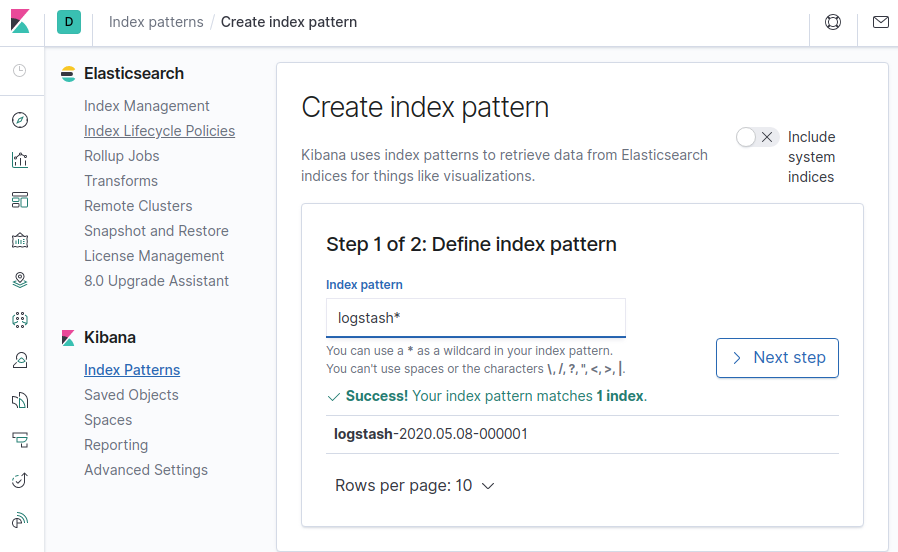
\includegraphics[width=11cm]{img/screenshots/kib_create_index_pattern.png}
    \caption{Création de l'index pattern dans Kibana}
    \label{f-kibCreateIndexPattern}
\end{figure}
Une fois créé, on peut voir les logs dans l'onglet \verb,Discover, de Kibana. Il est également possible d'afficher uniquement les champs qui nous intéressent, comme ceux créés dans le filtre.
\begin{figure}[H]
    \centering
    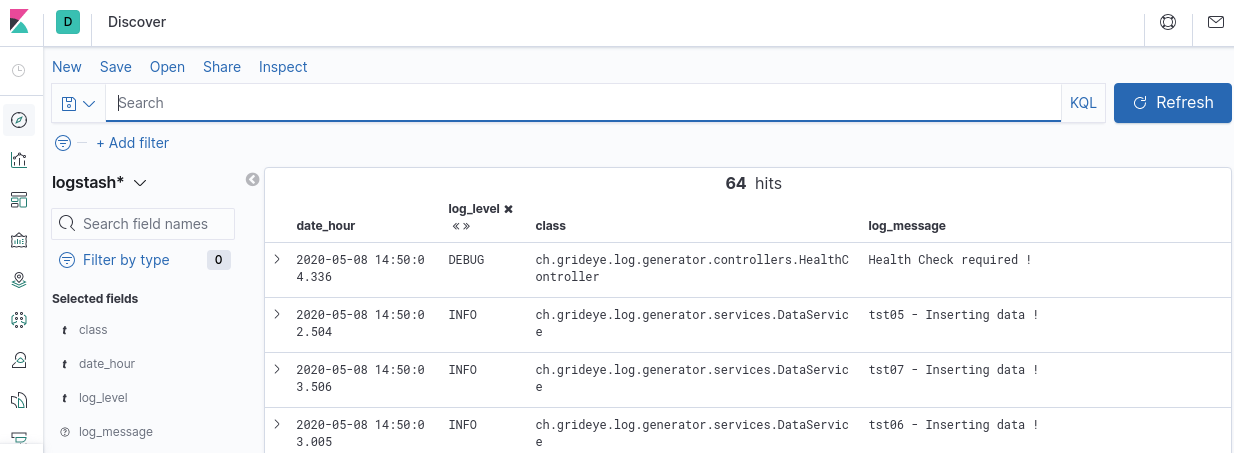
\includegraphics[width=18cm]{img/screenshots/kib_logs_arrived.png}
    \caption{Affichage des logs dans Kibana}
    \label{f-kibLogsArrived}
\end{figure}

\subsection{Visualisation avec Kibana} \label{ss-visualisationAvecKibana}

Une fois tous les outils installés, il ne reste plus qu'à créer des visualisations permettant de suivre l'état du système en temps réel, ou encore de retrouver l'origine d'un problème sur le système.

Pour ce faire, nous allons créer plusieurs visualisations, elles-même contenues dans des tableaux de bord.

Un premier tableau de bord montrera tous les problèmes de l'infrastructure. Ainsi, un opérateur pourra voir immédiatement s'il y a eu un problème dernièrement, ou au contraire si le tableau est vide.

Pour ce cas d'utilisation, il y aura ensuite un autre tableau de bord mettant en relation les taux d'utilisations CPU de chaque conteneur Docker. Il permettra, au cas où l'opérateur remarque une surcharge CPU sur le tableau de bord des problèmes, de déterminer quelle application pose problème.

\subsubsection{Tableau de bord des problèmes} \label{sss-tableauDeBordDesProblemes}

Pour ce tableau de bord, nous avons inséré quatre informations susceptibles d'être considérées comme des \og problèmes \fg :
\begin{itemize}
    \item Les logs de crash du simulateur GridEye
    \item Les redémarrages de conteneur Docker
    \item Les sur-exploitations du processeur
    \item Les sur-exploitations de la mémoire
\end{itemize}

La figure \ref{f-dashboardOfProblems} montre ce tableau de bord. Les trois premières visualisations, concernant les crashs du simulateur ainsi que les sur-exploitations sont de simples recherches dans les logs. Pour les crashs, on affiche tous les logs ayant le champ \verb,class, indiquant le service de crash. Pour le CPU, tous les logs de pourcentage d'utilisation CPU avec une valeur plus grande que 3 sont affichés (les pourcentages des 4 coeurs sont additionnés). Et pour l'utilisation de la mémoire, une valeur plus grande que 0.8 a été choisie. Pour la dernière visualisation, on a un tableau affichant le nombre de logs contenant l'information de Docker \verb,container status, à \verb,Up 2 minutes,.

Sur la capture d'écran de la figure \ref{f-dashboardOfProblems}, on peut voir un crash du simulateur, plusieurs logs de CPU sur-exploité, aucun pour la mémoire, et quelques redémarrages de conteneur. Pour les redémarrage conteneur, les premiers histogrammes correspondent au premier lancement de l'application, donc les redémarrages qui doivent être interprétés comme des erreurs sont seulement les suivants.

À la vue de ce tableau de bord, on peut donc rapidement conclure que dans l'heure qui précède, on a eu un crash, des problèmes de CPU et un redémarrage de conteneur.

\begin{figure}[H]
    \centering
    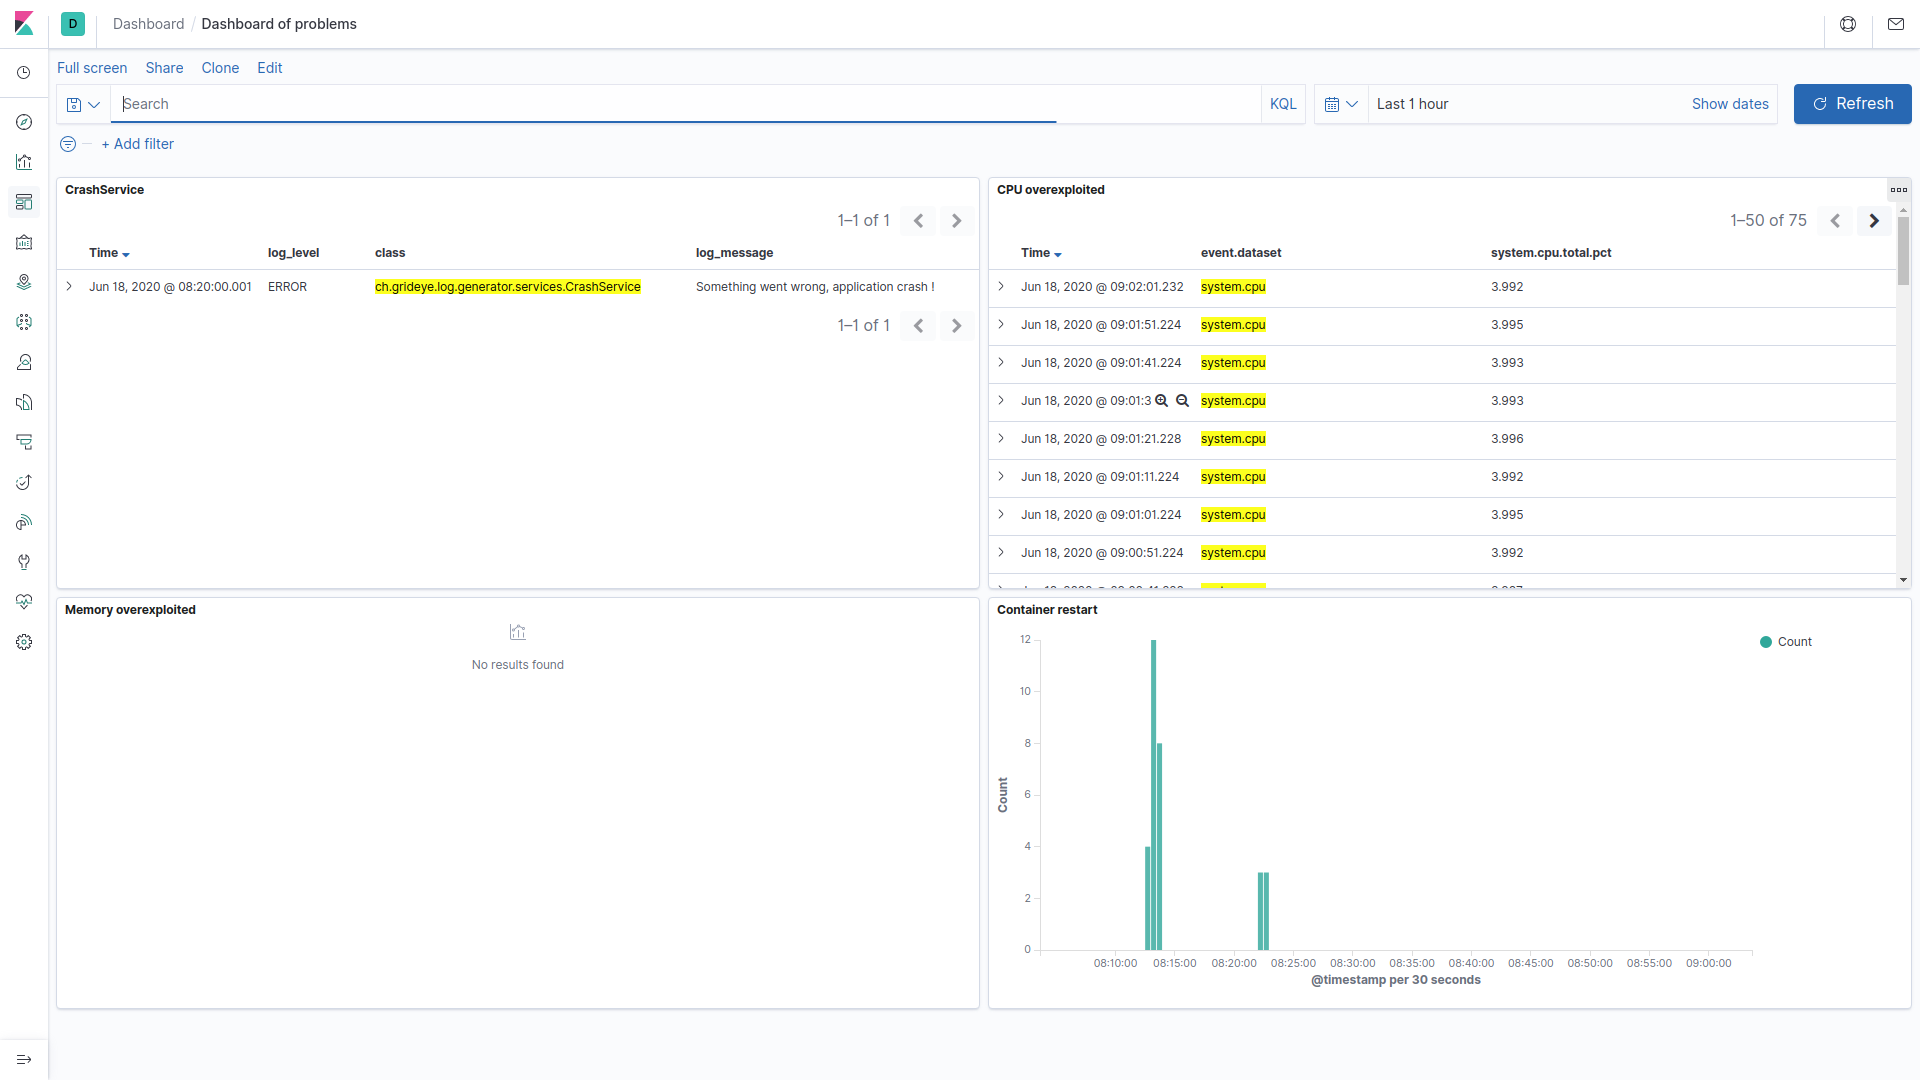
\includegraphics[width=18cm]{img/screenshots/dashboardOfProblems.png}
    \caption{Tableau de bord des problèmes - Kibana}
    \label{f-dashboardOfProblems}
\end{figure}

\subsubsection{Tableau de bord du CPU} \label{sss-tableauDeBordDuCPU}

Après avoir constaté ces différents problèmes, on pourrait imaginer que l'opérateur veuille s'attaquer à la surcharge du processeur, et voudrait en savoir un peu plus sur l'origine de cette anomalie. Un tableau de bord contenant les informations détaillées des consommations de CPU a donc été créé.

La figure \ref{f-dashboardOfCPU} montre ce tableau de bord.

Les valeurs d'utilisation du CPU sont les mêmes que dans le tableau des problèmes : les pourcentages des 4 coeurs sont additionnés. Elles varient donc de 0 à 4. Dans cette capture d'écran, on remarque que le problème vient du simulateur GridEye, car il utilise périodiquement les pleines capacités du CPU, alors que les trois autres conteneurs ne dépassent pas les 3\% sur la globalité des 4 coeurs. L'opérateur pourra encore pousser ces recherches en regardant les logs de GridEye aux heures où il consomme tout le processeur.

\begin{figure}[H]
    \centering
    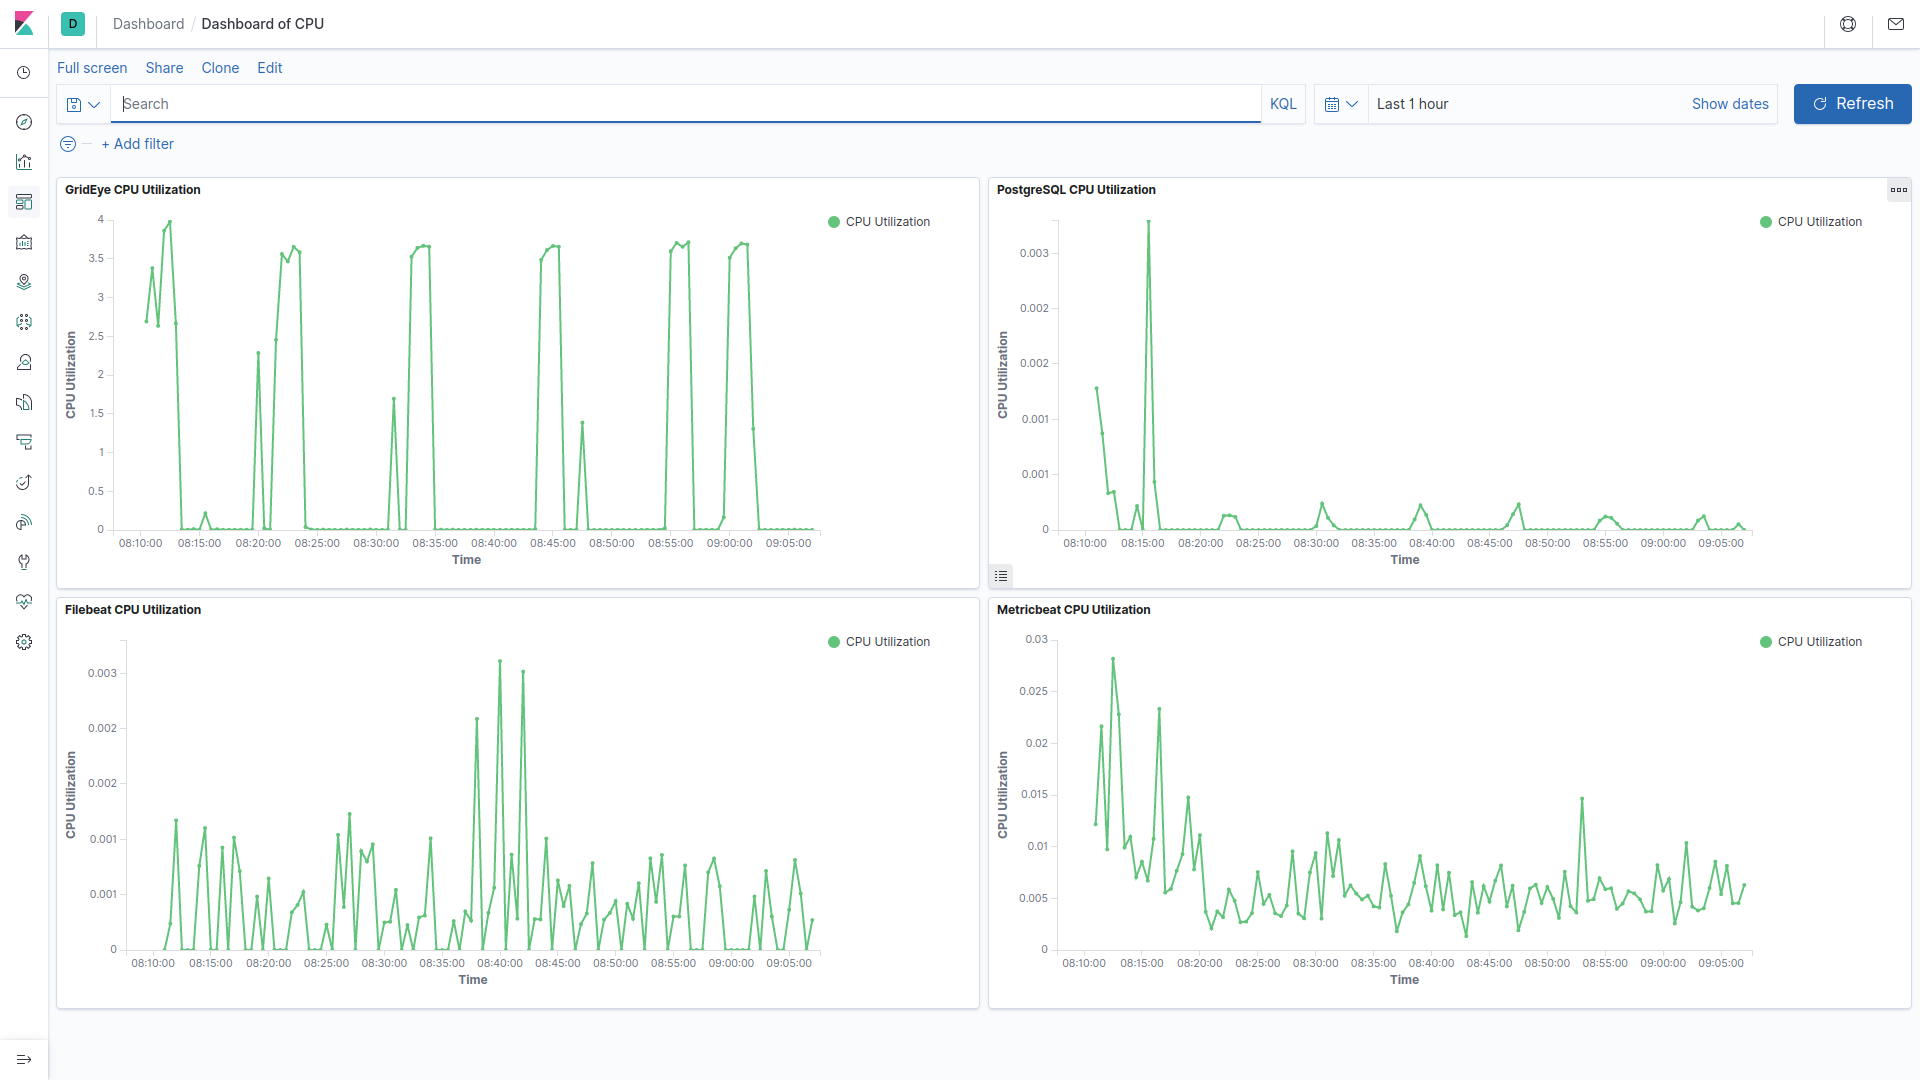
\includegraphics[width=18cm]{img/screenshots/dashboardOfCPU.png}
    \caption{Tableau de bord du CPU - Kibana}
    \label{f-dashboardOfCPU}
\end{figure}

\subsection{Amélioration de l'architecture Docker}
Des améliorations mineures ont été réalisées sur les fichiers \verb,Dockerfile, et \verb,docker-compose.yml,, notamment sur la manière de gérer les versions de la Suite Elastic, qui est passé de 7.6.2 au début du Travail de Bachelor à 7.8.0 à l'heure où ces lignes sont écrites. Ces fichiers se trouvent à l'annexe \ref{appendix:ss-versionAmelioreeDocker}. Les différents répertoire GitHub mentionnés dans ce rapport sont également à jour \cite{jael24_jael24tb_elasticstack_2020, jael24_jael24tb_fielddevices_2020, jael24_jael24tb_grideye_simulator_2020}.

\newpage

\section{Détection d'anomalies et corrélation d'événements} \label{s-detectionAnomaliesEtCorrelationEvenements}

Maintenant que la Suite Elastic est fonctionnelle, nous avons des données de logs et de métriques à disposition. L'étape suivante consiste à rendre ces données parlantes, à en tirer des informations utiles et éloquentes. Pour ce faire, plutôt que de simplement créer des visualisations et des tableaux de bord, nous allons utiliser des algorithmes évolués.\newline
Ceux-ci permettront de faire de l'analyse de métriques, ce qui permettra d'agir sur des problèmes de manière anticipée. Cette analyse de métrique s'appelle la \textbf{détection d'anomalies} (\textit{anomaly detection} ou \textit{outlier detection} en anglais). Formellement, la détection d'anomalies dans les séries temporelles a pour but de différencier les moments où une valeur est dite normale, ou anormale, puis de le signaler. Il y a plusieurs manières de définir la normalité. On peut, par exemple, 
être normal par rapport à soi-même, en prenant compte de ses états historiques. On pourra donc se dire anormal si notre valeur est trop différente par rapport aux valeurs habituelles. On peut également être normal par rapport aux autres. Si beaucoup de même composants ont un comportement similaire, et que notre comportement est bien différent, alors on sera anormal. La figure \ref{f-illustrationsAD} illustre cette notion. \newline
On voudra également faire de la prédiction de série temporelle, à savoir estimer la valeur qu'aura notre série dans X temps, en fonction de la tendance actuelle et passée.
Concrètement, dans ce projet, un exemple basique consiste en un disque mémoire qui se rempli petit à petit, nous aimerions être informé de son plein remplissage avant qu'il n'arrive, sachant qu'il y a un certain délai de remplacement. Nous aimerions également avoir des seuils d'alertes \og actifs \fg, qui s'adaptent à une courbe de série temporelle, plutôt que de devoir définir des seuils d'alerte constants, qui demandent une réflexion pour la valeur à fixer.\newline
Nous allons également étudier des algorithmes de corrélation entre différents événements, dans l'optique de découvrir les \og symptômes \fg des pannes les plus fréquentes. L'exemple ici serait de définir une surcharge du CPU comme étant une panne. Le but de l'algorithme serait alors de découvrir quels sont les événements qui arrivent les plus souvent avant cette panne. Il serait donc possible de donner une alerte avant la panne, qui donnerait un message de la forme \og symptôme X détecté, n\% de probabilité qu'une surcharge CPU suive \fg.\newline
Pour ce faire, une étude des différents algorithmes actuellement utilisés dans des cas similaires sera faite, afin de choisir les algorithmes les plus adaptés, puis une implémentation de ces-dits algorithmes sera réalisée.

\begin{figure}[H]
  \centering
  \subfloat[Anomalie par rapport à soi-même]{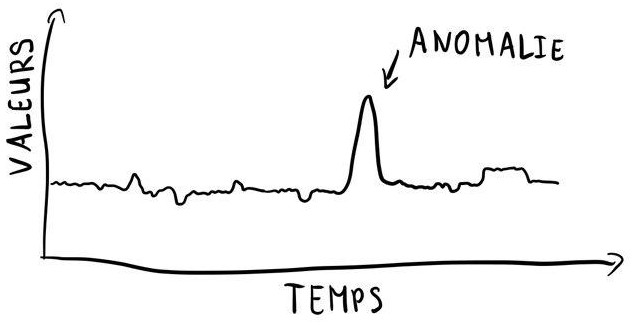
\includegraphics[width=0.4\textwidth]{img/AD_myself.jpg}\label{f-AD_myself}}
  \hfill
  \subfloat[Anomalie par rapport aux autres]{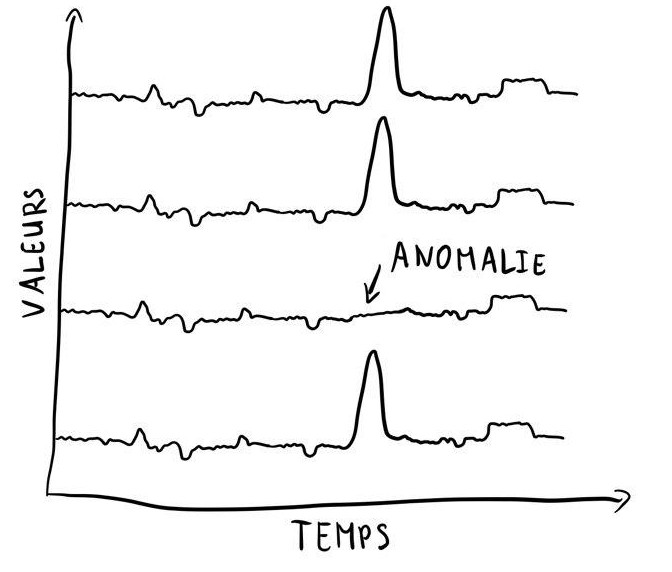
\includegraphics[width=0.4\textwidth]{img/AD_others.jpg}\label{f-AD_others}}
  \caption{Illustration de la détection d'anomalies - inspiré par \cite{noauthor_introduction_2019}}
  \label{f-illustrationsAD}
\end{figure}

\subsection{État de l'art}

Il existe de nombreux algorithmes dans le domaine de la détection d'anomalies, qui ont chacun leurs fonctionnalités, et leurs avantages et inconvénients. Chacun de ces algorithmes possède son propre but, et il n'y a pas de méthode permettant de faire de la prédiction, de l'adaptation de seuil actif et d'autres choses en même temps. Pour avoir un système complet, il faut donc utiliser et implémenter plusieurs algorithmes. Globalement, la détection d'anomalie n'est pas quelque chose de simple, et sa résolution est donc par définition complexe également. \newline
Pour commencer, il existe de nombreuse manière de détecter des anomalies dans une série temporelle. Il y aura des algorithmes basiques, ou des algorithmes d'apprentissage automatique. Dans cette dernière catégorie, il y aura des algorithmes à apprentissage supervisé ou non-supervisé, etc. Il faudra également choisir entre des algorithmes permettant d'analyser des séries temporelles historiques, ou d'autres qui permettent d'analyser des données en temps réel.
Globalement, pour déterminer l'algorithme à utiliser, il faut connaître sa série temporelle et savoir ce que l'on veut obtenir, afin de choisir le bon algorithme.

\subsubsection{Le Machine Learning de la Suite Elastic}
Dans le cadre de ce projet, comme la Suite Elastic est utilisée, et qu'elle propose elle-même des fonctionnalités de détection d'anomalies dans sa version Premium, le modèle à suivre sera tiré de cette suite. Toutes les fonctionnalités de détection d'anomalies se regroupent, chez Elastic, sous l'appellation \og Machine Learning \fg \cite{noauthor_machine_nodate}. Dans la version actuelle (7.8.0), la Suite Elastic propose de l'apprentissage automatique supervisé, et non-supervisé. La différence entre ces deux modes de fonctionnement est que pour utiliser les algorithmes supervisés, il faut fournir au système des données \og normales \fg, sans anomalies.\newline
Le Machine Learning d'Elastic est séparé en deux parties : \textit{Anomaly Detection}, qui est l'apprentissage automatique non-supervisé, et \textit{Data Frame Analytics}, qui lui est l'apprentissage automatique supervisé. La partie supervisée est pour l'instant expérimentale et Elastic n'exclut pas de la retirer totalement du produit dans le futur, ou de grandement la modifier, c'est pourquoi elle ne sera pas détaillée ici.

\paragraph{Anomaly Detection}
Dans le domaine du machine learning non-supervisé d'Elastic, on trouve également plusieurs fonctionnalités. Tout d'abord, la détection de normalité par rapport à soi-même et ses états passés. Cette fonctionnalité permet d'avoir des seuils dynamiques, et de définir quelles anomalies on veut détecter. On entend par là que la Suite Elastic propose des fonctions de détection. Par exemple, pour la surcharge CPU, seules les détections positives nous intéressent. En effet, si l'utilisation du processeur est trop basse (proche de 0\%), ce n'est pas un problème. La figure \ref{f-kibana_ADsingleMetric} montre une utilisation de cette fonctionnalité, avec une métrique d'utilisation CPU. On peut voir qu'après un certain temps, le modèle est calculé et adapte ses seuils dynamiquement. Il détecte alors des anomalies sur la deuxième surcharge CPU.

\begin{figure}[H]
    \centering
    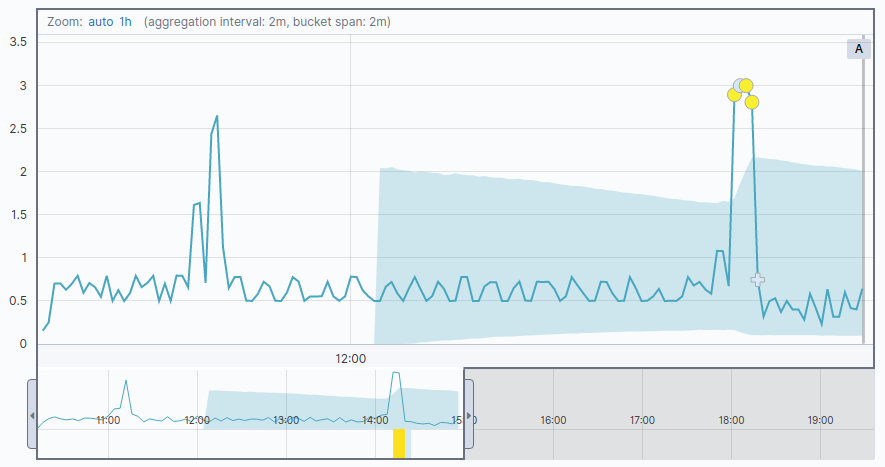
\includegraphics[width=18cm]{img/screenshots/AD_elastic_without_forecast.png}
    \caption{Kibana - Détection d'anomalies d'une métrique CPU}
    \label{f-kibana_ADsingleMetric}
\end{figure}

Avec cette même fonctionnalité, il est également possible d'effectuer une prédiction de valeurs, comme le montre la figure \ref{f-kibana_forecasting} (la prévision est la partie en jaune de la série temporelle). Avec cette image, on peut également constater qu'il faut que le modèle ingère quelques valeurs avant qu'il soit réellement opérationnel. En effet, au début de la série, les bornes sont très larges et ne suivent pas réellement la tendance. Ceci est dû, mise à part les propriétés de l'apprentissage automatique, au fait que le modèle est calculé au moment de l'ingestion. Il ne va en effet pas se calculer sur les données historiques, mais plutôt s'améliorer à chaque nouvelle donnée ingérée.

\begin{figure}[H]
    \centering
    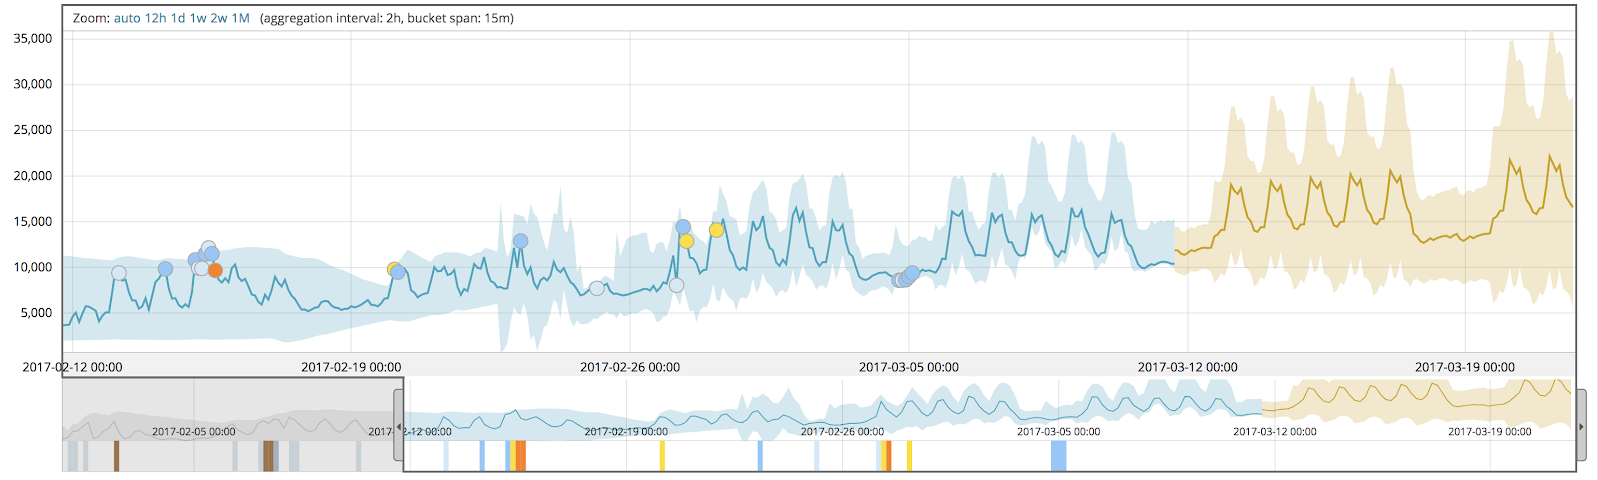
\includegraphics[width=18cm]{img/elastic_forecasting.png}
    \caption{Kibana - Prévision de valeurs \cite{noauthor_-demand_2018}}
    \label{f-kibana_forecasting}
\end{figure}

Une autre grande fonctionnalité de la détection d'anomalies est l'analyse de population, autrement dit, l'analyse de normalité par rapport aux autres, comme expliqué à la section \ref{s-detectionAnomaliesEtCorrelationEvenements}. Le but est donc d'avoir un grand nombre de machines, ou de composants de même type, afin de les analyser et de voir si un d'eux sort de la normalité. La figure \ref{f-kibana_ADpopulation} montre cette détection. On a plusieurs serveurs et l'information contenue dans le graphe est le nombre de requêtes reçues par l'adresse IP \verb,29.64.62.83,. On constate alors qu'un des serveurs en reçoit plus que les autres. Une anomalie est alors signalée.

\begin{figure}[H]
    \centering
    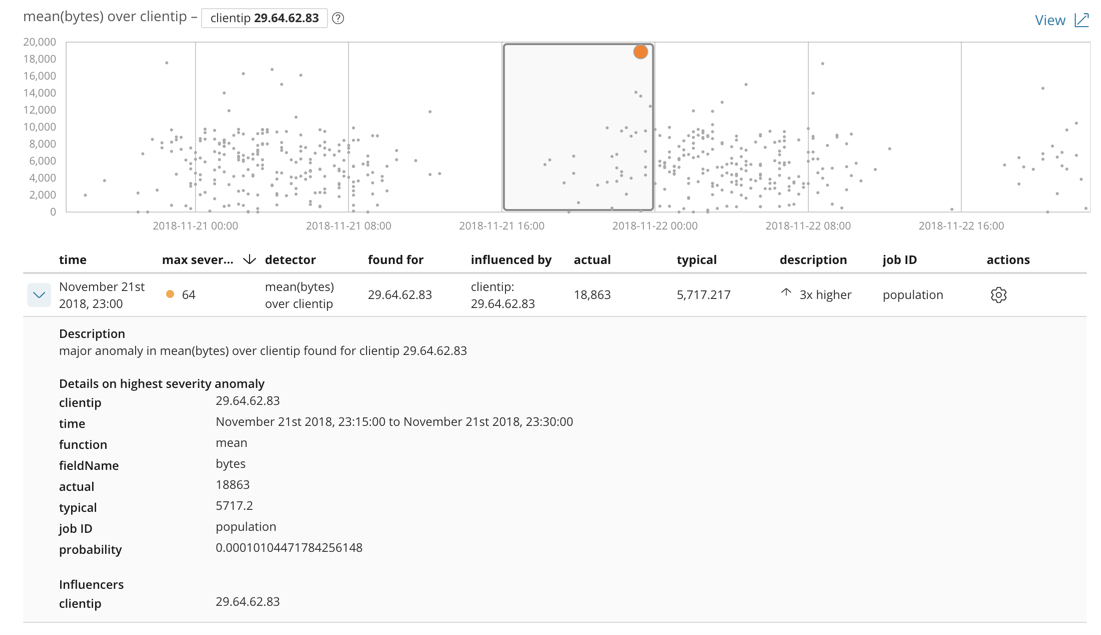
\includegraphics[width=18cm]{img/AD_elastic_population.jpg}
    \caption{Kibana - Détection d'anomalie dans une population \cite{noauthor_performing_nodate}}
    \label{f-kibana_ADpopulation}
\end{figure}

\paragraph{Data Frame Analytics}
La partie supervisée du Machine Learning d'Elastic contient, pour le moment, deux fonctionnalités. La première est une classification, et la deuxième est une régression. En théorie, la classification permet de faire de la prédiction de valeur discrète, en se basant sur d'autres données. Un exemple informatique est la classification des e-mails, entre \textit{spam} et \textit{ham}. En se basant sur plusieurs données dans le mail (heure d'envoi, texte, etc.), et connaissant un grand nombre d'e-mail étant des spam ou des ham, l'algorithme arrive à classer de nouveau mail dans une des deux catégories. \newline
Pour la régression, le principe est le même, à savoir s'entraîner sur des données pour prédire des nouvelles, mais cette fois sur des valeurs continues. L'exemple donné par Elastic est le prix d'un appartement. On connaît plusieurs données comme la surface habitable, la distance du centre-ville, etc. d'un grand nombre d'appartement, ainsi que leur prix. Et le programme arrive à déterminer le prix d'un autre appartement, en se basant sur ces mêmes critères (surface, distance, etc.). La figure \ref{f-illustrationsML} illustre ces deux fonctionnalités.

\begin{figure}[H]
  \centering
  \subfloat[Machine Learning - Classification]{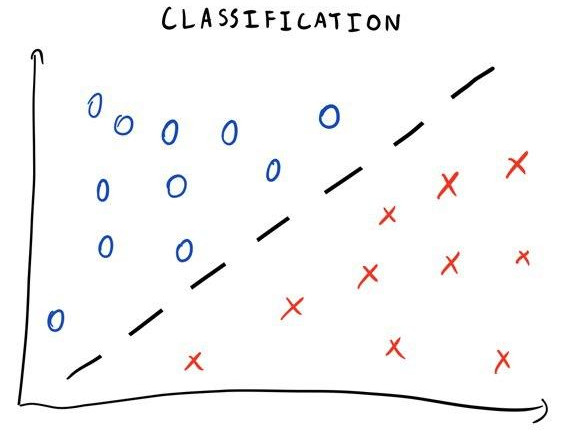
\includegraphics[width=0.4\textwidth]{img/ML_classification.jpg}\label{f-ML_classification}}
  \hfill
  \subfloat[Machine Learning - Régression]{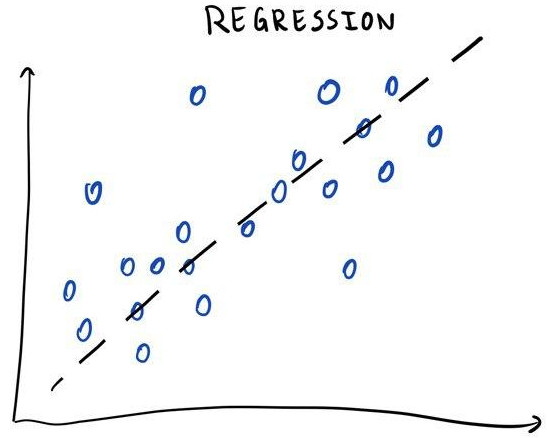
\includegraphics[width=0.4\textwidth]{img/ML_regression.jpg}\label{f-ML_regression}}
  \caption{Illustration des techniques d'apprentissage automatique}
  \label{f-illustrationsML}
\end{figure}

Le Machine Learning d'Elastic Stack est un de leur principaux axes de travail actuel. Il est amélioré et a été garni de nouvelles fonctionnalités avec beaucoup des derniers passages à de nouvelles versions. Il y aura donc probablement encore d'autres fonctionnalités qui vont venir s'y greffer dans les prochaines versions, ou des modifications aux possibilités actuelles.\newline
Comme il n'est pas possible dans les conditions d'un Travail de Bachelor d'implémenter autant de fonctionnalités que propose Elastic, il a été choisi de se focaliser sur la partie non-supervisée, qui serait la plus adaptée à notre projet. En effet, les seuils dynamiques sont une fonctionnalité qui apporte réellement un plus. Il y a plusieurs métriques à analyser sur la plateforme Smart Grid de DEPsys et il est compliqué de fixer un seuil supérieur et inférieur pour chacune de ces métriques. Cela demande une réflexion, puis un suivi non négligeable. Un algorithme non-supervisé permet alors d'annuler cette réflexion. De plus, pour utiliser des algorithmes supervisés, il est nécessaire de fournir au modèle une base assez conséquente de séries temporelle sans anomalie. Dans notre cas, nous n'avons pas ces données à disposition, et les générer demanderait un travail supplémentaire. \newline
La partie prédiction de l'apprentissage automatique non-supervisé est également intéressant. En étant combiné à un mécanisme d'alerte, elle s'inscrit dans la logique pro-active du système de gestion de logs, en anticipant les problèmes.\newline
Comme la Suite Elastic n'informe pas sur les algorithmes se cachant derrière les décors de leur Machine Learning non-supervisé, le vendant plus comme une fonctionnalité utilisable en quelques clics, une recherche sur les algorithmes actuellement les plus utilisés s'impose.

Voici quelques algorithmes, ou bibliothèques d'algorithmes, n'utilisant pas forcément l'apprentissage automatique, proposant une fonctionnalité de détection d'anomalies.

\subsubsection{Décomposition STL}
La décomposition STL basé sur Loess \cite{noauthor_regression_2018} n'est pas une méthode de détection d'anomalies à première vue, mais beaucoup d'algorithmes sont basés sur cette décomposition de signal. Concrètement, la plupart des séries temporelles sont saisonnières \cite{noauthor_seasonality_2020}, ce qui signifie qu'elles ont certaines variations qui se répètent tous les x temps, p. ex. chaque semaine. Un exemple typique est la baisse du nombre de requête sur un serveur en pleine nuit, alors qu'en journée le taux augmente. Cette décomposition consiste à séparer la série temporelle en 3 :
\begin{itemize}
    \item Saisonalité
    \item Tendance
    \item Bruit (reste du signal)
\end{itemize}
Après avoir décomposé une série, on peut détecter plus facilement les anomalies, ceci sur la courbe du bruit. En effet, l'algorithme ne sera plus perturbé par les variations de saisonalité et de tendance, qui ne sont pas des anomalies. Comme le montre la figure \ref{f-STLDecomposition}, sur le signal non décomposé, on ne voit pas forcément d'anomalie. Par contre, après décomposition, sur la série du bruit (\textit{remainder}) on constate clairement une baisse anormale en début de l'année 1952. 

\begin{figure}[H]
    \centering
    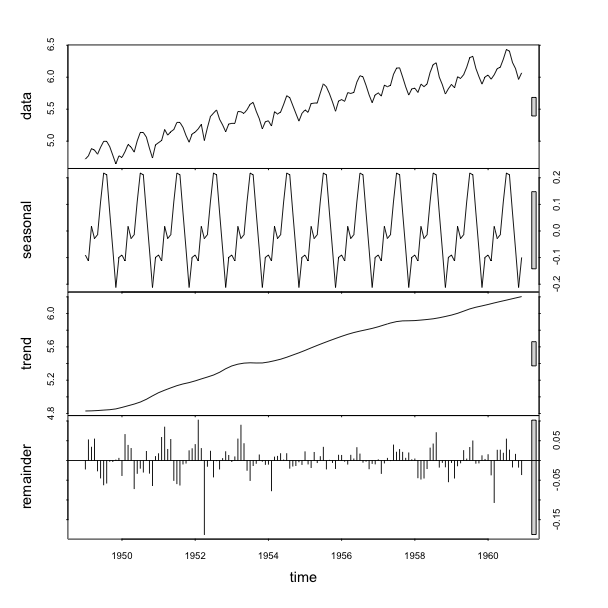
\includegraphics[width=18cm]{img/STL_decomposition.png}
    \caption{Décomposition STL d'une série temporelle \cite{wheeler_anomaly_2018}}
    \label{f-STLDecomposition}
\end{figure}

\subsubsection{ARIMA}

La méthode ARIMA \cite{noauthor_autoregressive_2020} permet de faire de la prédiction de valeurs de série temporelle.
Ce modèle est un algorithme d'apprentissage automatique qui est une contraction de plusieurs \og sous-modèles \fg. On compte d'abord le modèle AR, qui est un modèle auto-régressif. Ce type de modèle fonctionne sur le principe que les valeurs passées ont un impact sur les valeurs actuelles, ce qui permet de prédire une valeur selon les précédentes.\newline
Ensuite, il y a le modèle MA, qui est un modèle de moyenne mobile \cite{noauthor_moyenne_2020}. La moyenne mobile consiste à calculer la moyenne de \textit{n} termes d'une série (qui se nomme régulièrement une \textit{fenêtre}), puis de passer à la valeur suivante. On fait ainsi glisser la fenêtre de moyenne sur les valeurs de la série. La table \ref{t-ExempleMoyenneMobile} montre un exemple avec une fenêtre de taille n = 2.

\begin{table}[H]
\centering
\begin{tabular}{ |m{2cm}|m{2cm}|m{2cm}|m{2cm}|m{2cm}|m{2cm}|  }
    \hline
    Valeurs & 3 & 6 & 12 & 0 & 4 \\
    \hline
    Moyenne mobile & - & $\frac{3+6}{2} = 4.5$ & $\frac{6+12}{2} = 9$ & $\frac{12+0}{2} = 6$ & $\frac{0+4}{2} = 2$ \\
    \hline
\end{tabular}
\caption{Exemple de moyenne mobile}
\label{t-ExempleMoyenneMobile}
\end{table}

En combinant ces deux approches, on obtient alors un modèle ARMA. Et ARIMA ajoute un élément I, pour intégration, qui signifie que les valeurs de données ont été remplacées par la différence entre leurs valeurs et les valeurs précédentes. ARIMA est une généralisation du modèle ARMA. \newline
Globalement, la méthode est basée sur une approche selon laquelle plusieurs points du passé génèrent une prévision du point suivant, et avec l'ajout d'une variable aléatoire.

Chaque parties du modèle demande un paramètre, et donc la méthode ARIMA en demande trois, qui ne sont pas forcément facile à déterminer :
\begin{itemize}
    \item Le nombre de termes autorégressif (AR)
    \subitem Correspond à l'ordre du modèle auto-regréssif \cite{noauthor_processus_2020}
    \item Le nombre de différence non-saisonnière (I)
    \subitem Correspond aux nombres de fois que la différence a été soustraite à la valeur de donnée.
    \item Le nombre de termes moyens mobiles (MA)
    \subitem Correspond à la taille de la fenêtre de la moyenne mobile.
\end{itemize}

Une autre difficulté est que la série temporelle à analyser doit être stationnaire \cite{noauthor_stationnarite_2020}. Une série stationnaire est une série qui ne dépend pas du temps, la figure \ref{f-illustrationsStationnarite} illustre ce concept de stationnarité. Il est cependant possible de rendre une série stationnaire en appliquant une opération mathématique sur les valeurs, selon la non-stationnarité. Par exemple, pour une série qui croît proportionnellement au temps, on peut appliquer ARIMA sur le logs des valeurs.

\begin{figure}[H]
  \centering
  \subfloat[Série temporelle stationnaire]{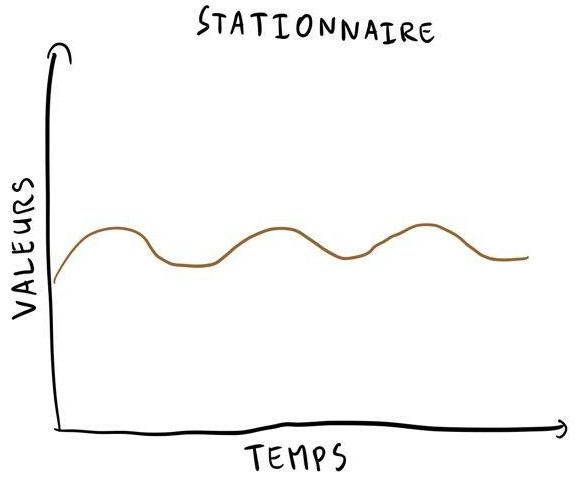
\includegraphics[width=0.4\textwidth]{img/Serie_stationnaire.jpg}\label{f-serieStationnaire}}
  \hfill
  \subfloat[Série temporelle non stationnaire]{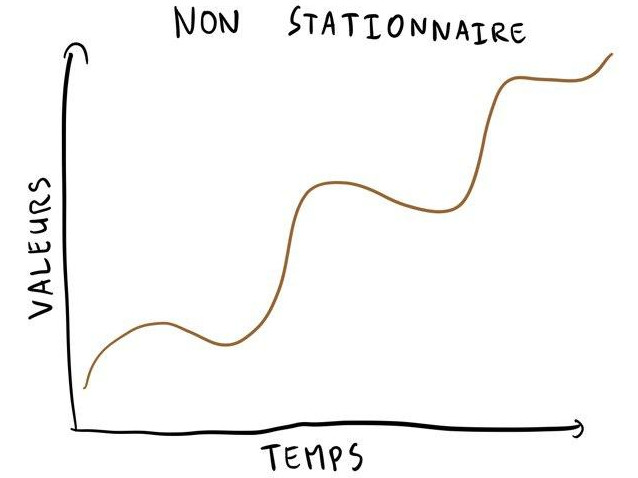
\includegraphics[width=0.4\textwidth]{img/Serie_non_stationnaire.jpg}\label{f-serieNonStationnaire}}
  \caption{Illustration de la stationnarité des séries temporelles}
  \label{f-illustrationsStationnarite}
\end{figure}


\subsubsection{Twitter AnomalyDetection}
Twitter a développé une bibliothèque de détection d'anomalies \cite{noauthor_twitteranomalydetection_2020, noauthor_introducing_nodate}, utilisant la décomposition STL, ainsi qu'un algorithme Seasonal Hybrid ESD (S-H-ESD), basé sur le test ESD généralisé \cite{noauthor_135173_nodate}, qui est utilisé pour détecter des valeurs aberrantes dans une série temporelle. \newline
Leur système permet de détecter aussi bien des anomalies globales que locales, tout comme des anomalies positives et négatives. Ces aspects sont montrés avec la figure \ref{f-TwitterAD}.

\begin{figure}[H]
    \centering
    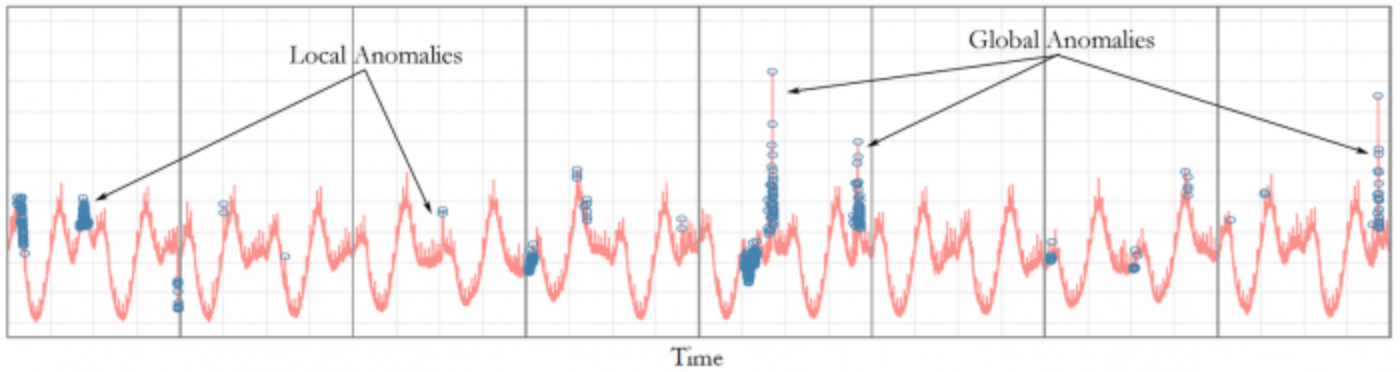
\includegraphics[width=18cm]{img/TwitterAD.png}
    \caption{Résultat de l'algorithme de Twitter pour la détection d'anomalie \cite{noauthor_introducing_nodate}}
    \label{f-TwitterAD}
\end{figure}

\subsubsection{Facebook Prophet}
Comme Twitter, Facebook a également développé une bibliothèque de détection d'anomalies, appelée Prophet \cite{noauthor_prophet_nodate}. Il est spécialisé dans la prédiction de valeurs dans des séries temporelle et est basé sur un modèle additif. Il est particulièrement adapté à des séries ayant une saisonalité marquée, et gère bien les données manquantes. La figure \ref{f-FacebookProphet} montre la bibliothèque Prophet en action sur une série temporelle de 8 ans, avec une prédiction de valeurs sur une année.

\begin{figure}[H]
    \centering
    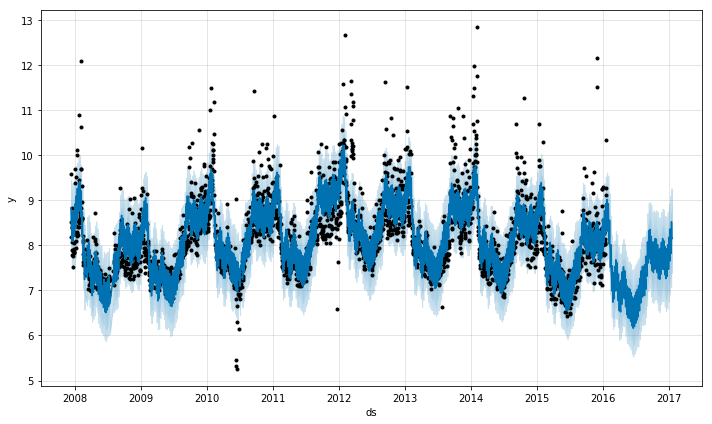
\includegraphics[width=18cm]{img/facebook_prophet.png}
    \caption{Résultat de l'algorithme de Prophet pour la détection d'anomalie \cite{noauthor_quick_nodate}}
    \label{f-FacebookProphet}
\end{figure}

\subsubsection{Autres algorithmes de détection d'anomalies}
Le domaine de la détection d'anomalies est réellement vaste et beaucoup d'article ainsi que de papier universitaire parlent de ce sujet. Il existe un répertoire GitHub \cite{zhao_yzhao062anomaly-detection-resources_2020} listant des ressources concernant cette thématique et qui est régulièrement mise à jour. Il existe également beaucoup d'autres d'algorithmes/bibliothèques/méthodes traitant de ce sujet que ceux qui ont été présentés dans ce document. En voici une liste non exhaustive :
\begin{itemize}
    \item Arbres de classification et de régression
    \subitem Apprentissage automatique, peux être utilisé en supervisé ou en non-supervisé. Permet de faire de la prédiction de séries temporelles.
    \item Algorithme de Welford
    \subitem Algorithme statistique qui peut être utilisé pour faire de la détection d'anomalie sur des flux de données (en temps réel) \cite{lobo_detecting_2020}.
    \item Boîte à moustaches
    \subitem Les boîtes à moustaches sont des outils statistiques très simples qui indiquent des valeurs médianes ainsi que des valeurs aberrantes. Ils peuvent être utilisés comme outil de détection d'anomalies \cite{lobo_detecting_2020}.
    \item Half-Space Tree (HST)
    \subitem Une méthode d'apprentissage automatique supervisé qui peut être utilisé sur des flux de données \cite{lobo_detecting_2020}.
    \item Long Short-Term Memory (LSTM)
    \subitem Consiste en un réseau de neurone récurrent \cite{noauthor_reseau_2020}.
\end{itemize}

\subsubsection{Corrélation d'événements}
Le domaine de la recherche de corrélation d'événements dans les outils de gestion de logs est moins développé que celui de la détection d'anomalies. Il n'existe pas, par exemple, de fonctionnalité dans la Suite Elastic permettant de trouver un \og symptôme \fg de panne. Par symptôme de panne, on entend un événement qui permet de deviner une panne à venir. Il y a également peu ou pas de papier universitaire parlant de cette thématique. Nous avons donc tenté d'utiliser un algorithme très utilisé dans le monde du commerce : l'analyse du ticket de caisse (plus connu sous le nom anglais de \textit{Market Basket Analysis}).

\paragraph{Market Basket Analysis} \label{paragraph-MBA}
Le but de cet algorithme est de lier des événements à des autres afin de déterminer des liens de type $EvenementA \rightarrow EvenementB$, avec la flèche voulant dire \og a pour conséquence \fg. Le côté gauche de la règle est \og l'antécédent \fg, alors que le côté droit est la \og conséquence \fg. Il est beaucoup utilisé dans le commerce afin d'organiser les rayons des magasins. Il nécessite d'enregistrer tous les tickets de caisse des clients, que l'on nommera \og transactions \fg, puis d'appliquer l'algorithme de Market Basket Analysis qui sortira les événements ayant le plus souvent lieu ensemble. Le but, dans un commerce, est de trouver l'organisation des rayons permettant de vendre le plus de produit possible. Par exemple, si on remarque que la plupart des clients qui achètent des couches pour bébé achètent également des bières, alors on disposera le rayon \og bières \fg à côté du rayon \og couches pour bébé \fg. \newline
Pour utiliser cet algorithme, on a besoin d'un set de donnée contenant des transactions. Une transaction est une liste d'événements ayant eu lieu ensemble. Dans le cas d'un commerce, une transaction est un ticket de caisse, car il renseigne une liste d'article ayant été acheté ensemble. Dans le cas de notre projet, la transaction sera des événements (logs) ayant eu lieu dans une certaine fenêtre de temps. Le résultat de l'algorithme sera des règles d'associations. Par exemple, $\{Bieres, Chips\} \rightarrow \{Couches\}$ signifie qu'un client qui achète des bières et des chips achète souvent des couches. Dans la même idée, la règle $\{AnalyseDisque\} \rightarrow \{SurchargeCPU\}$ indiquera qu'après une analyse de disque, une surcharge CPU à des grandes chances d'arriver. \newline
Les règles d'associations produite par l'algorithme sont accompagnées de trois métriques permettant d'évaluer la force de la règle : \cite{noauthor_market_2017}

\begin{itemize}
    \item Support
    \subitem Le pourcentage de transaction qui contient tous les éléments de la règle. Par exemple, pour la règle $\{Bieres, Chips\} \rightarrow \{Couches\}$, ce sera le pourcentage des tickets contenant les 3 articles bières, chips et couches. Il est donc préférable de se fier à des règles avec un haut niveau de support.
    \item Confiance
    \subitem La probabilité qu'une règle qui contient les mêmes antécédents (et peut-être d'autres) contient l'article conséquent dans sa partie de droite. Par exemple, dans notre cas, la probabilité qu'une règle qui contient, dans sa partie antécédent, entre autres, les articles bières et chips, a dans sa partie \og conséquence \fg l'article couches. Une grande confiance permet d'assurer la véracité de la règle.
    \item Lift
    \subitem On prend le support, et on le divise par les probabilités des éléments antécédents et conséquents, comme s'ils n'étaient pas liés par la règle. Cela permet de montrer la force de l'association entre les produits de gauche et de droite. Plus le lift est grand, plus le lien entre les deux parties est important.
\end{itemize}

Voici un exemple d'application simpliste de l'algorithme, adaptée à ce projet :

\begin{itemize}
    \item Soit une base de 1000 transactions contenant des événements normaux comme \og Analyse de disque \fg, \og transmission de logs \fg, ou encore \og insertions de données dans la BDD \fg, et des événements problématiques comme \og surcharge CPU \fg, \og surcharge RAM \fg, ou encore \og crash Java \fg.
    \item Dans ces transactions, 127 d'entre elles contiennent une analyse de disque, 43 une surcharge CPU et 37 les deux.
    \item On analyse la règle $\{AnalyseDisque\} \rightarrow \{SurchargeCPU\}$.
    \item Le support sera $P(analyse \cap surcharge) = \frac{37}{1000} = 0.037$
    \item La confiance sera $\frac{support}{P(analyse)} = \frac{0.037}{0.127} = 0.29$
    \item Le lift sera $\frac{support}{P(analyse)\cdot P(surcharge)} = \frac{0.037}{0.127 \cdot 0.043} = 6.78$
\end{itemize}

L'algorithme peut donc être utilisé dans d'autres cas que celui du commerce. Cependant, la notion de transaction est moins évidente qu'un ticket de caisse lorsqu'il s'agit de logs et de problèmes comme des pannes. Il faut tout d'abord définir les problèmes à analyser, puis créer les transactions avec des fenêtres temporelles, en utilisant le même principe que pour la moyenne mobile, tel que montré avec la table \ref{t-ExempleMoyenneMobile}. Il faut donc déterminer la taille de la fenêtre permettant d'obtenir un problème et sa cause. Ce n'est pas quelque chose de trivial et cela demande une certaine analyse manuelle.\newline
Une autre contrainte de cette méthode est le nombre de donnée à mettre à disposition de l'algorithme. En effet, plus il y aura de donnée, plus il sera performant. En l'occurrence, comme notre cas d'utilisation est sensé découvrir la causalité de problèmes, et que les problèmes ne sont pas sensés arriver de manière nombreuse, il sera forcément plus difficile d'entraîner l'algorithme que dans le cas d'un ticket de caisse, qui est une transaction banale.

\subsection{Implémentation}

Après avoir analysé les différentes possibilités théoriques permettant d'avoir une analyse semblable à celle de la Suite Elastic, vient l'étape d'implémentation. Trois fonctions présentant donc trois algorithmes ont été réalisées. Elles ne sont pas directement liées avec un mécanisme d'analyse en temps réel sur les données du simulateur GridEye. Ces fonctions permettent de créer un résultat d'analyse statique sur des données, soit directement lues dans Elasticsearch, soit dans un fichier \verb,CSV, annexe.

\subsubsection{ARIMA}
L'algorithme ARIMA ici utilisé permet de faire de la prédiction de valeur de série temporelle. Il lit en entrée un fichier \verb,CSV, contenant les données à analyser. Elle applique ensuite l'algorithme et affiche sur un graphe le résultat.

Le fichier \verb,CSV, est de la forme montrée dans la table \ref{t-ExempleCSVARIMA}.

\begin{table}[H]
\centering
\begin{tabular}{ |m{4cm}|m{4cm}|  }
    \hline
    Date & Valeurs \\
    \hline
    "2020-07-01 08:13:57" & 3.763 \\
    \hline
    "2020-07-01 08:14:07" & 1.033 \\
    \hline
    "2020-07-01 08:14:17" & 0.308 \\
    \hline
    "2020-07-01 08:14:27" & 0.556 \\
    \hline
    "2020-07-01 08:14:37" & 0.535 \\
    \hline
    ... & ... \\
    \hline
\end{tabular}
\caption{Exemple fichier CSV de données pour l'algorithme ARIMA}
\label{t-ExempleCSVARIMA}
\end{table}

Voici le code de la fonction : \cite{noauthor_modearima_2020}

\begin{lstlisting}[language=python]
def arima_forecast(csv_file, start_plot, end_plot, arima_parameters):
    """Compute a forecasting operation with an ARIMA algorithm on a timeseries read in a CSV file"""
    df = pd.read_csv(csv_file, parse_dates=['Date'], index_col=['Date'])

    model = ARIMA(df, order=arima_parameters)
    results = model.fit(disp=-1)
    fig = results.plot_predict(start_plot, end_plot)
    fig.show()
\end{lstlisting}

Cette fonction prend en paramètre le nom du fichier \verb,CSV, les bornes dans lesquelles les données doivent être analysée, ainsi que les paramètres de la fonction ARIMA. La fonction ARIMA utilisée est celle de la bibliothèque \verb,statsmodels, \cite{noauthor_introduction_nodate}.
Les résultats sont relativement bons sur des données qui vont bien, par exemple l'historique des passagers en avion dans les années 50-60, car la série est croissante et le programme arrive à prédire les valeurs de manière intéressante, comme le montre la figure \ref{f-ARIMAResultAirlines}. Comme nous ne disposons pas de données comparables relative au système GridEye, il n'est malheureusement pas possible de le tester. Sur des données plus \og plates \fg, comme l'utilisation CPU, le résultat ne donne rien d'utilisable, comme le montre la figure \ref{f-ARIMAResultCPU}.

\begin{figure}[H]
    \centering
    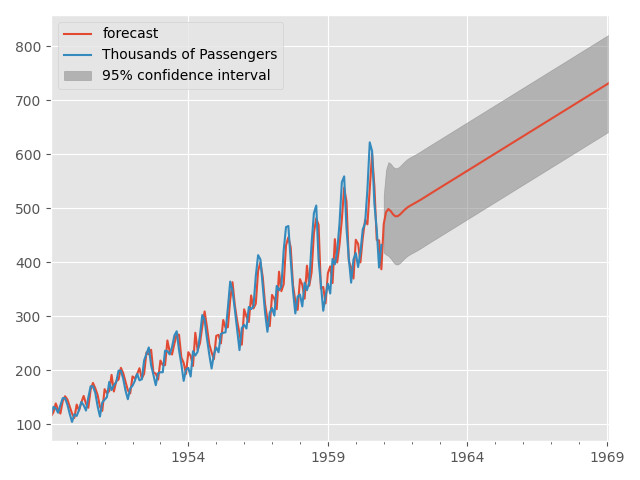
\includegraphics[width=15cm]{img/ARIMA_forecast_aircraft.jpg}
    \caption{Résultat de l'algorithme ARIMA sur des données de passagers de vols}
    \label{f-ARIMAResultAirlines}
\end{figure}

\begin{figure}[H]
    \centering
    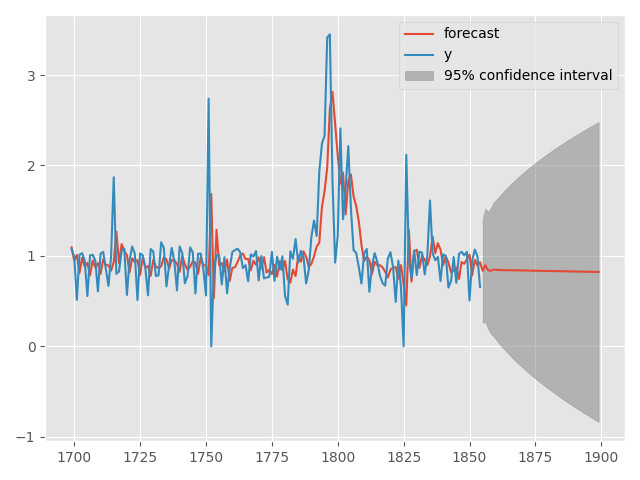
\includegraphics[width=15cm]{img/ARIMA_forecast_cpu.jpg}
    \caption{Résultat de l'algorithme ARIMA sur des données de CPU}
    \label{f-ARIMAResultCPU}
\end{figure}

\subsubsection{Facebook Prophet}

Dans notre cas, l'utilisation de la librairie Prophet de Facebook permet de faire de la détection d'anomalie grâce à des seuils actifs. Les fonctions implémentées prennent un fichier \verb,CSV, en entrée, puis montrent le résultat dans un graphe. Le fichier \verb,CSV, en entrée doit obligatoirement contenir une colonne \verb,ds, contenant les dates, et une autre colonne \verb,y, contenant les données, comme le montre la table \ref{t-ExempleCSVProphet}.

\begin{table}[H]
\centering
\begin{tabular}{ |m{4cm}|m{4cm}|  }
    \hline
    "ds" & "y" \\
    \hline
    "2020-07-01 08:13:57" & 3.763 \\
    \hline
    "2020-07-01 08:14:07" & 1.033 \\
    \hline
    "2020-07-01 08:14:17" & 0.308 \\
    \hline
    "2020-07-01 08:14:27" & 0.556 \\
    \hline
    "2020-07-01 08:14:37" & 0.535 \\
    \hline
    ... & ... \\
    \hline
\end{tabular}
\caption{Exemple fichier CSV de données pour l'algorithme de Prophet}
\label{t-ExempleCSVProphet}
\end{table}

L'annexe \ref{appendix:prophetPy} montre le code du programme utilisant Facebook Prophet \cite{ashrapov_anomaly_2020}.


Sur un set de donnée CPU généré sur un machine faisant tourner le simulateur GridEye pendant plusieurs heures, Prophet arrive à obtenir de bons résultats, que l'on peut voir à la figure \ref{f-ProphetCPU}. On peut également voir que Prophet gère bien les trous de données. En effet, entre 13h05 et 13h50, il n'y a aucune donnée présente, et tout reprend normalement par la suite.

\begin{figure}[H]
    \centering
    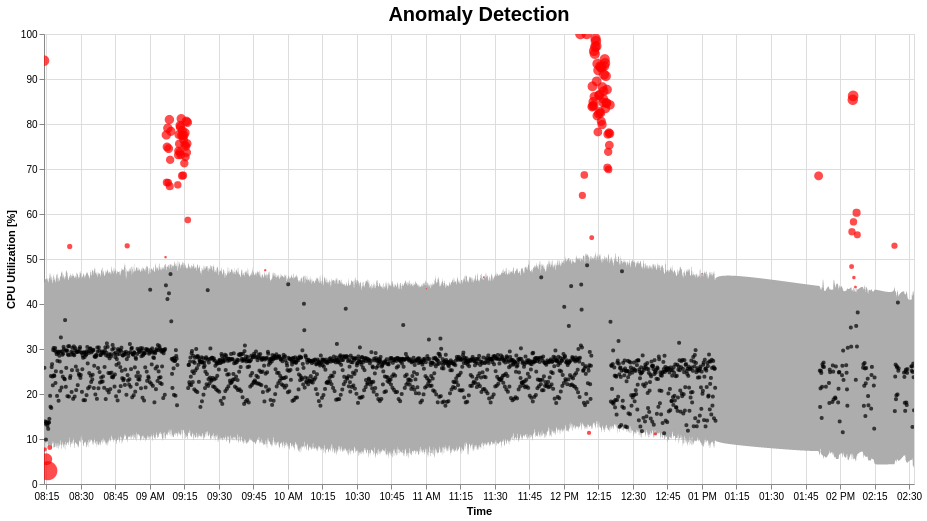
\includegraphics[width=18cm]{img/AD_prophet_CPU.png}
    \caption{Résultat de l'algorithme de Prophet sur des données de CPU}
    \label{f-ProphetCPU}
\end{figure}

\subsubsection{Market Basket Analysis}
L'implémentation du Market Basket Analysis n'a pas donné de résultats probants. En effet, comme décrit à la section \ref{paragraph-MBA}, il est très difficile d'utiliser un algorithme de Market Basket Analysis sans un grand set de donnée. Ce code fonctionne donc en théorie, mais n'a pas été testé avec des données liées au projet.

Voici le code python de la fonction : \cite{noauthor_introduction_nodate-1}

\begin{lstlisting}[language=python]
def market_basket_analysis(logs, transaction):
    """Compute a market basket analysis on the logs stored in the class."""
    list_articles = list(logs)

    list_occ = []

    for k, v in transactions.items():
        list_occ.append([])

        for article in list_articles:
            list_occ[k].append(v[article] if (article in v) else 0)

    df = pd.DataFrame(list_occ, columns=list_articles)

    frequent_itemsets = apriori(df, min_support=0.05, use_colnames=True)
\end{lstlisting}

Cette fonction prend des logs, qui correspondent aux différents \og articles \fg, en reprenant l'analogie avec le monde du commerce. C'est donc un \verb,set, qui contient tous les logs existants. La fonction prend également une liste de transactions, qui est une \verb,map, ayant pour clé un id de transaction, et pour valeur une nouvelle \verb,map,, qui elle a pour clé un log, puis pour valeur un 0 si le log est absent dans la transaction, et un 1 s'il est présent.\newline
L'algorithme \verb,apriori, utilisé, qui est la base du Market Basket Analysis, est celui de la librairie mlxtend \cite{raschka_mlxtend_2018}. Il est ensuite possible de créer des règles pour trouver des informations de la manière suivante :
\begin{lstlisting}[language=python]
# Create the rule
rules = association_rules(frequent_itemsets, metric="lift", min_threshold=1)
\end{lstlisting}

Le code permettant d'aller chercher ces informations de logs et de transactions est disponible à l'annexe \ref{appendix:retrieveLogsPy}. 
    
\newpage

\section{Conclusion}

Après cette étape d'implémentation vient la conclusion et donc la fin de ce Travail de Bachelor. Cette conclusion sera en trois parties. Tout d'abord, une conclusion purement technique sur les choses réalisées par rapport aux demandes du cahier des charges. Suivra une conclusion personnelle et mon avis sur le travail réalisé. Puis, pour finir, une liste des améliorations possibles.

\subsection{Conclusion technique}
Dans les grandes lignes, le cahier des charges demandait une évaluation des différents système de gestion de logs, afin de mettre en place une solution pour l'infrastructure GridEye de DEPsys.
Si on s'en tient aux demandes du cahier des charges, on peut conclure que pour la première partie, à savoir la comparaison, les différentes étapes réalisées ont été pertinentes. Elles nous ont permis de choisir un système, la Suite Elastic, qui offre toutes les fonctionnalités dont nous sommes en mesure d'attendre d'un système de gestion de logs, tout en proposant un environnement flexible et agréable à utiliser. Sa documentation, que ce soit dans les instructions d'installations, ou dans les notices d'utilisations de fonctionnalités comme le Machine Learning, est riche et à jour. Ils proposent, de plus, un bon nombre de vidéos \og webinars \fg, en anglais et en français, expliquant par l'exemple l'utilisation de leurs services. \newline
Toujours en suivant le cahier des charges, la suite mentionnée est la mise en place de la solution pour l'infrastructure GridEye. À nouveau, on peut conclure que les différentes installations réalisées sont intéressantes, de part leur nature \og dockerisée \fg, elles sont flexibles est faciles de mise en fonction. \newline
La dernière étape du cahier des charges mentionne l'implémentation de librairies pour l'interfaçage avec le Back-End de la solution GridEye. À ce niveau-ci, le travail a plutôt été réalisé avec un simulateur de la plateforme GridEye, étant donné la difficulté technique pour interfacer un PoC avec la solution GridEye. En effet, GridEye n'est pas encore prête à générer des logs et d'autres événements pertinents à un niveau permettant d'être utilisé et testé avec une démonstration de faisabilité. De plus, la situation sanitaire liée au coronavirus n'aide pas à une telle manoeuvre, étant donné que les différentes parties ne se sont pas rencontrées chez DEPsys. \newline
Au delà des spécifications du cahier des charges, si on s'en tient aux différentes demandes évoquées lors du Travail de Bachelor, on peut conclure que la première partie a été remplie (installation avec Docker, respect du cas d'utilisation, etc.). Pour la partie implémentation des algorithmes avancés, sensés permettre de détecter des anomalies ou de trouver des corrélations entre les événements, une disparité entre les attentes et les résultats peut se faire ressentir. En effet, nous sommes loin des fonctionnalités de la partie Machine Learning de la Suite Elastic.

\subsection{Conclusion personnelle}

Pour ma part, dans la globalité du Travail de Bachelor, je suis plutôt content du résultat. Premièrement, dans la grande majorité des tâches effectuées, j'ai pris du plaisir à découvrir de nouvelles technologies que je ne connaissais pas. Dans la première partie, lors de l'évaluation des différents systèmes de gestion de log, j'ai découvert un nouveau monde, le monde du log, qui à première vue n'est pas le plus passionnant des domaines de l'informatique, mais qui cache une grande complexité et un potentiel pas assez exploité. Ensuite, lors de la réalisation de la démonstration de faisabilité, j'ai pu créer deux architectures mêlant Docker et Docker-compose. Ce sont des technologies que je connaissais mais que je n'avais jamais utilisée \og de zéro \fg, en créant son propre \verb,Dockerfile, et \verb,docker-compose.yml, partant d'un fichier vide. Ces expériences m'ont servi et m'ont plu. La partie suivante, qui consistait en des recherches et implémentations d'algorithmes de détection d'anomalies, m'a ouvert quelque peu le monde de la \og Data Science \fg, dans lequel j'ai pu remarquer que mes connaissances mathématiques étaient enfouies très loin dans ma mémoire.\newline
Si j'ai grandement apprécié découvrir ces différents domaines, le trop plein de nouvelles connaissances s'est probablement emparé de moi dans les dernières semaines, et il devenait difficile d'avancer sereinement de plusieurs pas, sans devoir refaire des pas en arrière suite à de mauvais choix effectué par manque de connaissance, ou peut-être d'un manque de soif d'apprendre encore de nouvelle chose. \newline
Je pense que j'aurais été plus à l'aise avec un Travail de Bachelor portant sur un projet de réalisation de Back-end, ou la réalisation d'une application Java, mais je n'aurai pas ouvert mon horizon comme j'ai pu le faire avec ce projet, et je pense qu'il est important de le faire. C'est également pourquoi j'ai d'autant plus apprécié le suivi constant de Nastaran, ainsi que de Jonathan et Pascal, que je remercie chaleureusement pour leurs nombreux conseils.\newline
Au niveau technique, je pense que toutes les parties, hors implémentation des algorithmes de détection d'anomalies, sont utilisables. J'en suis donc heureux, même si je regrette de n'avoir pas pu aller plus loin dans ces algorithmes. Je pense toutefois que le défi était trop grand pour une personne seule dans le temps imparti. En effet, la grandeur du domaine de la détection d'anomalies, et la lecture d'article implique un temps énorme pour comprendre ces algorithmes, pouvoir choisir lequel utiliser et en faire un programme fonctionnel avec la solution GridEye.

\subsection{Améliorations possibles}
Je pense que la plupart des améliorations peuvent se faire dans l'analyse des logs et la mise en relation des informations obtenues dans ces logs. On pourrait donc imaginer réaliser des implémentations fonctionnelles des différents algorithmes présentés à la section \ref{s-detectionAnomaliesEtCorrelationEvenements}, qu'ils fonctionnent en temps réel, et que les modèles s'améliorent constamment. \newline
Pour l'architecture actuelle de la Suite Elastic, il faudrait rendre persistant la base de données Elasticsearch. Il faudrait éventuellement gérer la rétention des logs. Il faudrait également rendre persistant les visualisations et les tableaux de bord générés.


\newpage

\thispagestyle{empty}
\centering
\vspace{10cm}
{\huge ANNEXES}
\addcontentsline{toc}{section}{Annexes}


\newpage

\appendix
\renewcommand\thesection{\Alph{section}}

\addtocontents{toc}{\protect\setcounter{tocdepth}{1}}

\justify

\listoftables
\addcontentsline{toc}{section}{Liste des tableaux}
\newpage

\listoffigures
\addcontentsline{toc}{section}{Table des figures}
\newpage

\addcontentsline{toc}{section}{Références}
\printbibliography
\newpage

\section{Fichiers}

\subsection{logstash.conf}
\label{appendix:logstashConf}
\lstinputlisting[language=bash]{files/logstash.conf}

\subsection{filebeat.yml}
\label{appendix:filebeatConf}
\lstinputlisting[language=bash]{files/filebeat.yml}
Remplacer \verb,<REPOSITORY>, par la localisation du répertoire contenant le fichier de logs.\\
Remplacer \verb,<IP>, par l'adresse IP de la machine sur laquelle Logstash tourne.

\subsection{filebeat.yml de l'image Docker pour l'implémentation du cas d'utilisation}
\label{appendix:filebeatConfDockerUC}
\lstinputlisting[language=bash]{files/filebeat_docker_UC.yml}

\subsection{metricbeat.yml de l'image Docker pour l'implémentation du cas d'utilisation}
\label{appendix:metricbeatConfDockerUC}
\lstinputlisting[language=bash]{files/metricbeat_docker_UC.yml}

\subsection{docker-compose.yml du côté terrain pour l'implémentation du cas d'utilisation}
\label{appendix:dockercomposeFieldUC}
\lstinputlisting[language=bash]{files/docker-compose_field_UC.yml}
Remplacer \verb,<DOCKER_FIELD_PATH>, par la localisation du répertoire contenant l'arborescence de la machine \og terrain \fg.\\

\subsection{prophet.py}
\label{appendix:prophetPy}
\lstinputlisting[language=python]{files/prophet.py}

\subsection{retrieve\_logs.py}
\label{appendix:retrieveLogsPy}
\lstinputlisting[language=python]{files/retrieve_logs.py}

\subsection{Version améliorées des topologies Docker} \label{appendix:ss-versionAmelioreeDocker}

\subsubsection{Côté ELK}

\paragraph{docker-compose.yml}
\lstinputlisting[language=bash]{files/dc_ELK_nouveau.yml}
\paragraph{Dockerfile elasticsearch}
\lstinputlisting[language=bash]{files/Dockerfile_elsearch_nouveau}
\paragraph{Dockerfile kibana}
\lstinputlisting[language=bash]{files/Dockerfile_kib_nouveau}
\paragraph{Dockerfile logstash}
\lstinputlisting[language=bash]{files/Dockerfile_logst_nouveau}

\subsubsection{Côté terrain}

\paragraph{docker-compose.yml}
\lstinputlisting[language=bash]{files/dc_field_nouveau.yml}
Remplacer \verb,<PATH>, par la localisation du répertoire contenant l'arborescence de la machine \og terrain \fg.\\
\paragraph{Dockerfile filebeat}
\lstinputlisting[language=bash]{files/Dockerfile_fb_nouveau}
\paragraph{Dockerfile metricbeat}
\lstinputlisting[language=bash]{files/Dockerfile_mb_nouveau}


\newpage



\section{Détails des tests}

\subsection{Tests de débit d'ingestion}

Graylog (3.2.4 Virtual appliance) avec Filebeat :

Sans extractor (module de Graylog permettant le parsing des logs) :

Début du chargement : 10:09:17 \\
Fin du chargement : 10:09:24 \\
Temps de chargement : 7 secondes \\
Débit moyen : \textasciitilde 14'043,47 EPS \\

Avec extractor :

Début du chargement : 07:46:47.153 \\
Fin du chargement : 07:46:59.648 \\
Temps de chargement : 12.495 secondes \\
Débit moyen : \textasciitilde 7'867,55 EPS \\

Elastic Stack sans Logstash :

Début du chargement : 10:34:34.200 \\
Fin du chargement : 10:35:03.622 \\
Temps de chargement : 29.422 secondes \\
Débit moyen : \textasciitilde 3'341,21 EPS \\

Elastic Stack complet (sans filtrage du log) :

Début du chargement : 10:44:11.851 \\
Fin du chargement : 10:44:31.920 \\
Temps de chargement : 20.069 secondes \\
Débit moyen : \textasciitilde 4'898,35 EPS \\

Elastic Stack complet (avec filtrage du log) :

Début du chargement : 10:26:37.308 \\
Fin du chargement : 10:26:48.015 \\
Temps de chargement : 10.707 secondes \\
Débit moyen : \textasciitilde 9'181,38 EPS \\

Splunk :

Avec filtrage : \\
Donné (metrics.log de Splunk) : 2'628 EPS \\

Solarwinds Loggly avec endpoint bulk :
Avec Loggly, il est impossible de charger un fichier de plus de 5 MB. Il a donc été réduit à 3'999 lignes.

Début du chargement : 08:42:11.360 \\
Fin du chargement : 18:42:12.224 \\
Temps de chargement : 0.864 seconde \\
Débit moyen : \textasciitilde 46'295,14 EPS \\

\section{Journal de travail}


\subsection{Jeudi 13 février}
    Première réunion avec Nastaran, Jonathan et Pascal. Jonathan et Pascal ont expliqué leur vision du TB à travers une présentation, puis nous avons planifié le travail de Bachelor. Notamment les dates de fin d'évaluation (avec la présentation à DEPsys), et de fin de développement du use-case.
\subsection{Mercredi 19 février}
    Début du Travail de Bachelor. J'ai commencé par suivre un tuto afin de maîtriser les bases du langage \LaTeX, ce qui me sera utile pour tout ce qui est rédactionnel. Ensuite, j'ai commencé à revoir la présentation de Pascal afin de bien comprendre (notamment les technologies que je ne connais pas).
\subsection{Jeudi 20 février}
    J'ai regardé plusieurs vidéos qui présentent les différentes technologies que je dois évaluer.
\subsection{Mercredi 26 février}
    J'ai décidé de commencer à évaluer plus en profondeur Elasticsearch en premier, car Prometheus à comme contrainte de ne pas gérer les logs textuels, mais uniquement des métriques numériques. Cependant, d'après plusieurs lectures, je pense qu'il pourrait être intéressant de mixer les deux solutions. J'ai donc installé les outils de la suite ELK, et suivi des tutos plus concret en ce qui concerne Elasticsearch (insertion de donnée, recherches, etc.).
\subsection{Jeudi 27 février}
    Deuxième réunion avec Nastaran. Elle me propose de recentrer mes recherches sur la partie \og Log Analysis \fg, donc rechercher directement l'intégration de l'analyse de logs avec ELK par exemple. Après la réunion, j'ai donc continué mes recherches dans ce sens et ai suivi la vidéo d'Elastic qui concerne l'analyse de logs.
\subsection{Mercredi 04 mars}
    J'ai commencé à écrire ce journal afin de mieux me rappeler de ce que j'ai fais, ainsi que d'être plus structuré. Je commence également à utiliser Zotero, qui permet d'enregistrer tous les liens que je trouve intéressants, ainsi que de créer une bibliographie. J'ai également décidé de m'intéresser à Graylog en plus de ELK.
\subsection{Jeudi 05 mars}
    J'ai exploré plus en profondeur les articles de type \og Elastic Stack versus Graylog \fg, et je vais donc inclure la stack \og Graylog server, MongoDB et Elasticsearch \fg dans le comparatif. Cette suite-là me semble très appropriée au traitement et à l'analyse de logs.
    J'ai été à la réunion avec Nastaran à 11h30. Suite à cette réunion, nous avons décidé qu'il fallait que je fasse une synthèse des mes recherches et que je la présente en quelques slides le jeudi 12 mars.
\subsection{Lundi 09 mars}
    J'ai commencé à faire la synthèse de mes recherches. Je vais donc la faire en 3 étapes :
    \begin{enumerate}
    \item Choix des critères d'évaluations
        \begin{enumerate}
            \item Selon des recherches au sujet des caractéristiques d'un \og Log Management Tool \fg
        \end{enumerate}
    \item Choix des outils à évaluer
        \begin{enumerate}
                \item Pour cette étape, je vais consulter plusieurs classements de système de gestion de logs et choisir ceux qui sont le plus souvent cités. Je vais probablement en prendre 5 ou 6.
        \end{enumerate}
    \item Synthèse et rédaction des slides
    \end{enumerate}
    Ce lundi, j'ai défini les critères d'évaluation, selon les demandes de DEPsys ainsi que les critères lu lors de mes recherches.
\subsection{Mercredi 11 mars}
    J'ai fais un tableau pour le choix des outils à tester. J'ai donc effectué un classement selon 4 tops de système de gestion de logs.
    J'ai également commencé l'évaluation à proprement parler, en particulier sur Elastic Stack et Graylog. J'ai également eu un problème de stockage de la base de donnée Zotero et j'ai perdu toute ma bibliographie.
\subsection{Jeudi 12 mars}
    J'ai continué l'évaluation avec Loggly, j'ai créé la présentation de synthèse pour la réunion avec Nastaran, puis je l'ai présentée.
\subsection{Mercredi 18 mars}
    J'ai remis en place Zotero, cette fois avec une synchronisation en ligne de ma bibliographie. J'ai analysé les différents systèmes de gestion de logs que j'hésitais à inclure dans l'évaluation. J'ai donc écarté ManageEngine EventLog Analyzer pour sa popularité vraiment faible et son manque de documentation, et PRTG Network Monitor, qui est très axé sur l'analyse d'un réseau, comme son nom l'indique. Je vais donc évaluer Splunk.
\subsection{Jeudi 19 mars}
    J'ai fais l'évaluation de Splunk. J'ai également eu la réunion hebdomadaire avec Nastaran.
\subsection{Samedi 21 mars}
    J'ai reformaté mon rapport avec le template \LaTeX écrit par Mateo Tutic. J'ai également développé la partie Choix des différents systèmes à évaluer.
\subsection{Dimanche 22 mars}
    J'ai continué la partie Choix des différents systèmes à évaluer. J'ai également téléchargé la Suite Elastic et testé avec les logs systèmes de Ubuntu. Cela fonctionne normalement.
\subsection{Lundi 23 mars}
    J'ai mis en place les systèmes de gestion de logs Elastic Stack, Graylog, Splunk et Loggly. J'ai testé (en insérant des logs et regardant le débit) les 3 premiers. Encore quelques problèmes pour Loggly (pour l'instant, il sauvegarde 1 log avec n lignes dans le message plutôt que n logs avec 1 ligne). J'ai également terminé les tableaux récapitulatifs de l'évaluation de chaque système.
\subsection{Mardi 24 mars}
    J'ai terminé les tests d'ingestions de logs pour les 4 systèmes. J'ai commencé à faire mes slides pour la présentation du 25 mars.
\subsection{Mercredi 25 mars}
    J'ai terminé les slides de la présentation. J'ai fais la présentation du travail de Bachelor à l'entreprise DEPsys. S'en est suivi une discussion avec Pascal, Jonathan, Nastaran et moi au sujet de la suite de l'évaluation de mon TB, puis un ajustement du cas d'utilisation à implémenter fourni par Pascal.
\subsection{Jeudi 26 mars}
    J'ai commencé à refaire des tests d'ingestion de log. Cette fois-ci avec tout le pipeline. Je commence avec Elastic Suite, en y intégrant Logstash afin qu'il filtre les données.
\subsection{Mercredi 01 avril}
    J'ai continué les tests d'ingestion avec Elastic Stack et rencontré beaucoup de problème. J'arrive à faire fonctionner un pipeline Logstash-Elasticsearch-Kibana, et un pipeline Filebeat-Elasticsearch-Kibana, mais pas un contenant les 4 logiciels de la suite.
\subsection{Jeudi 02 avril}
    J'ai continué les tests en tentant plusieurs tutoriaux trouvé sur internet. Mais je rencontre toujours des problèmes. Ils sont probablement liés à la communication entre Filebeat et Logstash. J'ai également suivi les tuto officiels de la Suite Elastic, mais ça n'a pas fonctionné non plus. Ceci est peut-être dû à mes fichiers de configurations des logiciels Filebeat et Logstash. J'ai ensuite eu une réunion avec Nastaran.
\subsection{Mercredi 08 avril}
    J'ai continué les tests d'ingestion. En suivant les guides du site d'Elastic, j'ai remarqué qu'il y avait toute une section expliquant l'utilisation de la Suite avec Docker. Je me suis dit qu'il y avait plus de chance que cela fonctionne étant donné l'uniformité que propose Docker. Malheureusement, j'ai toujours les mêmes problèmes. Même en prenant un git public sensé fonctionner. Je me dit alors que le problème vient peut-être de mes fichiers de logs de tests (ils contiennent le même log multiplié n fois).
\subsection{Jeudi 09 avril}
    Je suis repassé sur une version non dockerisée de la Suite Elastic. J'ai téléchargé un fichier de log d'un serveur Apache afin de tester la Suite avec un fichier de log réel, et fait d'autres modifications, notamment sur les fichiers de configuration (j'ai créé la partie \og filtrage \fg de Logstash avec un site internet permettant de créer ces filtres de manière incrémentale). Et ça à fonctionné. J'ai ensuite eu la réunion avec Nastaran.
\subsection{Lundi 13 avril}
    J'ai effectué les tests de performances avec filtrage de la Suite Elastic. Après ceci, je me suis lancé dans les tests avec filtrage de Graylog. Cette fois-ci, ce n'est pas avec un logiciel intermédiaire comme Logstash, mais avec une fonctionnalité intégrée à Graylog : les Graylog Extractors.
\subsection{Mercredi 15 avril}
    J'ai commencé à cherché une façon d'effectuer le filtrage avec le système de gestion de logs Splunk. Malheureusement, j'ai l'impression que cela va être plus compliqué car Splunk favorise l'extraction des informations après l'indexage. Je vais encore chercher une journée, et si ce n'est pas concluant, je passerai outre.
\subsection{Jeudi 16 avril}
    J'ai tenté d'effectuer l'extraction d'informations dans les logs durant la phase de "parsing" du pipeline de Splunk. J'ai vu qu'il devait être possible de le faire en modifiant des fichiers de configuration dans le répertoire de Splunk, mais cela n'a pas fonctionné.
\subsection{Lundi 20 avril}
    J'ai rédigé les résultats des tests d'ingestion. J'ai ensuite commencé à étudié les manières de faire des tests de consommation CPU. Sachant qu'avec Amazon Web Service (AWS), comme je l'avais vu quelques semaines plus tôt dans un cours de Cloud Computing, il est possible de monitorer différentes métriques d'une instance, entre autres l'utilisation du CPU, je me suis lancé dans une installation de la Suite Elastic sur une instance t2.micro d'AWS. Malheureusement, ces instances sont trop petites et ne supportent pas simplement Elasticsearch. Ne voulant pas payer pour des instances plus grosses, je me suis rabattu sur la solution locale. Je vais donc simplement stopper le maximum de processus et monitorer l'utilisation de mon CPU avec l'outil natif d'Ubuntu. Je dois aussi installer Filebeat et Graylog sur un autre ordinateur afin de pouvoir faire ces tests (dans la réalité, le serveur et le client ne seront pas sur la même machine).
\subsection{Mercredi 22 avril}
    J'ai effectué les tests de consommation CPU de la Suite Elastic, de Graylog, ainsi que de Filebeat. J'ai ensuite commencé à rédiger la synthèse de ces tests.
\subsection{Jeudi 23 avril}
    J'ai continué la rédaction, j'ai ajouté le test d'ingestion d'un grand nombre de logs, la comparaison de popularité.
\subsection{Vendredi 24 avril}
    J'ai rédigé le cahier des charges, puis ai eu une réunion avec Nastaran. Nous avons discuté du cahier des charges, des améliorations à y apporter. Ensuite, nous avons un peu regardé l'état du rapport actuel. Il faut entre autres pense a y ajouter les références (tableaux, image, bibliographie). Nous avons ensuite convenu de fixer une réunion avec Jonathan et Pascal afin de leur présenter les résultats de l'évaluation. J'ai donc fixé cette réunion au jeudi 30 avril.
\subsection{Mercredi 29 avril}
    J'ai modifié le rapport pour y ajouter les références sur les tableaux et sur les figures. J'ai également amélioré les annexes avec la table des tableaux et la table des figures. J'ai également commencé la conclusion finale de l'évaluation, en rédigeant le paragraphe concernant l'analyse théorique.
\subsection{Jeudi 30 avril}
    J'ai continué le rapport. J'y ai ajouté une conclusion finale à l'évaluation. J'ai ensuite eu une réunion avec Pascal, Jonathan et Nastaran. Je leur ai présenté les résultats de mon évaluation et nous avons convenu ensemble d'effectuer l'implémentation du cas d'utilisation avec le système Elastic Stack.
\subsection{Mercredi 6 mai}
    J'ai pris en main le programme de Jonathan qui simule l'infrastructure GridEye de façon minimale. Je l'ai modifié légérement pour qu'il stocke les logs dans un fichier, plutôt que de les afficher dans la console. J'ai ensuite commencé à rédiger la partie implémentation du cas d'utilisation dans le rapport, tout en testant les commandes que je met dans le rapport sur une installation neuve d'Ubuntu.
\subsection{Jeudi 7 mai}
    J'ai continué la rédaction et la réalisation de l'implémentation du use case. J'ai rédigé les parties installations de la Suite Elastic, Configuration de la Suite Elastic.
\subsection{Vendredi 8 mai}
    J'ai continué la rédaction et la réalisation de l'implémentation du use case. J'ai maintenant un pipeline entier qui fonctionne avec le simulateur GridEye. J'ai également décrit tout cela dans le rapport. J'ai complété la bibliographie.
\subsection{Mercredi 13 mai}
    Je me suis lancé dans la dockerisation de la Suite Elastic. J'ai commencé par le faire avec 3 images Docker séparée, que je lançais avec un Docker run, comme indiqué dans la documentation. Cela fonctionnait bien avec Elasticsearch et Kibana, mais Logstash n'arrivait pas à communiquer avec Elasticsearch. J'ai remarqué que ceci était dû à la séparation des conteneurs effectuée par Docker. En effet, il n'était pas possible pour Logstash d'atteindre Elasticsearch avec l'adresse localhost, car pour le conteneur Logstash, il n'y a que lui sur \og son \fg localhost. J'ai donc décidé de passer à une topologie avec un docker-compose. Ayant plus d'expérience avec les configurations docker-compose que les simples commandes Docker, je pouvais plus facilement créer les liens entre les différentes applications. J'ai donc créé une topologie faisant communiquer toutes les applications de la Suite Elastic. J'ai ensuite rédigé mon rapport et j'y ai inclus un schéma montrant cette topologie.
\subsection{Jeudi 14 mai}
    J'ai continué le rapport avec la partie ELK et l'installation avec Docker et docker-compose. J'ai ensuite commencé à faire un schéma similaire pour la partie terrain, qui est un peu plus complexe. J'ai envoyé une première idée du schéma à DEPsys et Nastaran ainsi que mes questions, comme le rôle de la base de donnée PostgreSQL dans cette architecture. J'ai également eu une réunion avec Nastaran.
\subsection{Mercredi 20 mai}
    Après avoir reçu des réponses sur mes questions ainsi que l'approbation de Pascal quant à mon schéma. Je me suis lancé dans la réalisation de la topologie du côté terrain. J'ai décidé de construire mon conteneur Docker contenant l'application Java du simulateur GridEye à partir d'un fichier \verb,.jar,. J'ai eu quelques problèmes avec le fichier de logs dans lequel le simulateur doit écrire ses logs, et l'agent filebeat lire. J'ai rapidement compris qu'il me fallait là un Volume Docker partagé entre les deux conteneurs.
\subsection{Jeudi 21 mai}
    Je me suis renseigné sur les Volume Docker et leur intégration avec docker-compose. J'en ai donc intégré dans mon architecture pour partager le fichier de logs entre le simulateur GridEye et Filebeat. J'ai continué la réalisation de la topologie côté terrain avec l'intégration de Metricbeat et PostgreSQL.
\subsection{Mercredi 27 mai}
    En vue de la réunion du 28 mai, qui a pour but de présenter mes avancées dans l'implémentation du cas d'utilisation, j'ai terminé la topologie Docker du côté terrain, et ait tout fait fonctionné ensemble (terrain et ELK). J'ai aussi commencer à créer mes premières visualisations et tableau de bord (dashboard) dans Kibana. J'ai également avancé le rapport.
\subsection{Jeudi 28 mai}
    J'ai tenté de lancer un deuxième \og device terrain \fg à l'aide d'une machine virtuelle. Le test s'est bien passé. J'ai ensuite préparé ma présentation, et fait ma présentation à Jonathan, Pascal et Nastaran. Lors de cette réunion, DEPsys était globalement content de l'avancée et de l'architecture mise en place, qui correspondait à leurs attentes. Les prochaines étapes pour le cas d'utilisation étaient principalement situées dans le dashboard de Kibana, afin de créer, par exemple, un dashboard des problèmes, permettant à un opérateur de voir rapidement si une anomalie est présente, ou a été présente, dans le système.
\subsection{Jeudi 4 juin}
    J'ai avancé le rapport, dans lequel j'avais pris un peu de retard suite aux nombreuses implémentations pour le cas d'utilisation.
\subsection{Mercredi 10 juin}
    J'ai commencé à faire des corrections sur le pipeline de Logstash, par exemple faire en sorte que le tag \verb,_grokparsefailure, ne se mette plus sur les logs de metricbeat, ou encore utiliser la date des logs applicatifs comme \verb,time filter,.
\subsection{Jeudi 11 juin}
    J'ai continué les corrections du 10 juin. J'ai également eu une réunion avec Nastaran qui m'a parlé d'algorithme permettant de trouver des corrélations entre les événements, comme le \og market basket analysis \fg.
\subsection{Mercredi 17 juin}
    En vue du rendu du rapport intermédiaire (19 juin), j'ai relu tout le rapport, et modifié certaines parties. J'ai principalement supprimé la partie d'installation de la Suite Elastic sans Docker, qui me semblait peu pertinente. Et j'ai corrigé les fautes d'orthographe/grammaire/etc.
\subsection{Jeudi 18 juin}
    J'ai eu une réunion avec Nastaran, Pascal et Jonathan, dont le but était de parcourir le rapport pour voir s'il leur convenait pour le rapport intermédiaire. Il en est ressorti qu'il était ok, je dois juste modifier l'introduction, et faire une conclusion. Après cette réunion, j'ai donc fait ces deux parties.
\subsection{Vendredi 19 juin}
    J'ai relu et corrigé une dernière fois le rapport intermédiaire avant de le rendre.
\subsection{Mardi 23 juin}
    J'ai commencé aujourd'hui le TB à plein temps (nous avons encore des choses à rendre pour les autres cours d'ici ce soir, c'est pourquoi je n'ai pas avancé plus ces deux premiers jours). J'ai pris en compte les remarques que Pascal m'avait envoyées par mail concernant mon rapport intermédiaire. J'ai donc modifié le rapport par rapport à ses suggestions.
\subsection{Mercredi 24 juin}
    J'ai continué avec ce que j'avais décrit dans la section "suite" de mon rapport intermédiaire. Il y a d'abord des petites améliorations à faire. Je me suis lancé dans l'amélioration des fichiers de configurations, notamment de logstash, et j'ai directement remarqué que la Suite Elastic était passé de la version 7.6.2 utilisé lors de la première partie à la version 7.8.0. J'ai donc fait en sorte de passer à la dernière version en date.
\subsection{Jeudi 25 juin}
    J'ai décidé de rendre plus simple le passage de version, comme la Suite Elastic va encore changer. J'ai donc dans un premier lieu tenté de le faire avec un fichier \og .env \fg. et la fonctionnalité \verb,ENV, de docker/docker-compose, mais j'ai par la suite remarqué que pour ce cas d'utilisation, avec cette architecture, il fallait plutôt utiliser la fonctionnalité \verb,ARG,, qui n'est pas compatible avec les fichiers \og .env \fg. Cela n'est pas aussi bien que ce je voulais au début, mais je préfère ça que de devoir changer l'architecture.
    J'ai eu un premier rendez-vous avec Nastaran depuis le début du travail à plein temps. Elle m'a donné ses conseils/remarques concernant le rapport intermédiaire. Nous avons ensuite fixé un nouveau rendez-vous pour mardi prochain (30 juin).
\subsection{Vendredi 26 juin}
    J'ai continué avec la modification des problèmes \og mineurs \fg, comme le parsing des logs applicatifs, notamment au niveau de la date. Je me suis lancé la-dessus, avec le module \verb,date, de Logstash, mais j'ai rencontré des problèmes. Comme, à priori, je m'attendais à ce que ce genre de correction soit rapide et ne me cause pas de perte de temps, ce qui n'a pas été le cas, je vais, dès la semaine prochaine, m'attaquer aux algorithmes dont nous avons parlés (Market Basket Analysis p. ex.). Ce sont des choses plus centrales du TB, et si le temps me le permet, je reviendrai sur les petites choses comme la date des logs à la fin.
\subsection{Lundi 29 juin}
    J'ai fais des recherches sur les deux algorithmes dont Nastaran m'avait parlé : le Market Basket Analysis, qui devrait permettre de trouver une causalité entre différents événements. Et ARIMA, qui lui devrait permettre de prédire des dépassements de seuils selon les valeurs actuelles d'une \textit{time series}. Je garde aussi en tête ce qu'avait dit Pascal : le but est de transformer les métriques que l'on a actuellement en des visualisations montrant des incidents. Après mes recherches du jour, je conclue qu'il y a deux possibilités principales : Soit je développe moi-même des algorithmes comme MBA ou ARIMA, soit on utilise la version Premium de la Suite Elastic. J'ai regardé quelques vidéos d'Elastic présentant son Machine Learning, qui a l'air très performant, mais qui a un coût. Un développement perso serait gratuit, mais forcément moins bon.
\subsection{Mardi 30 juin}
    J'ai eu un rendez-vous avec Nastaran, dans lequel nous avons conclu qu'il fallait continuer les recherches, commencer à implémenter les algorithmes. J'ai donc continué mes recherches en essayant de trouver des articles incluant des implémentations d'algorithmes. J'ai également choisi de développer en Python, qui est un langage adapté à ce type d'algorithme (machine learning).
\subsection{Mercredi 1 juillet}
    J'ai commencé l'implémentation de l'algorithme de Market Basket Analysis. J'ai décidé de le tester avec le problème de la surcharge CPU. Pour l'instant j'ai des problèmes avec la manière de l'exécuter, notamment pour créer des \og transactions \fg, qui correspondent aux tickets de caisse dans la version pour les magasins. J'essaie de le faire en direct, en lisant les nouveaux logs toutes les 10 secondes.
    Mais il faut donc récupérer les logs arrivés plus tôt pour créer une transactions avec les causes d'un problème, et le problème en lui-même.
\subsection{Jeudi 2 juillet}
    J'ai continué l'implémentation du Market Basket Analysis, et j'ai décidé de faire des \og fenêtres glissantes \fg qui permettent de créer les transactions. J'ai également décidé de travailler sur l'ensemble des logs et pas uniquement sur les logs en direct, ce qui me permet d'avoir plus de données. J'ai ensuite eu un rendez-vous avec Nastaran. Je lui ai expliqué mon avancée tant dans mon implémentation que dans mes recherches. Nous avons conclu qu'il fallait dans un premier temps finir l'implémentation avec les fenêtres glissantes, malgré les résultats qui ne s'annoncent pas excellent, ceci étant dû principalement à la faible quantité de données. Le MBA est un algorithme qui demande un grand nombre de donnée pour être efficace. Dans un deuxième temps, il faudra que je me renseigne plus en profondeur sur les algorithmes utilisés par la version Premium de la Suite Elastic, et éventuellement l'essayer. Puis, dans un troisième temps, de me renseigner sur l'algorithme ARIMA, qui permet de prédire des valeurs dans le futur. Nous avons fixé le prochain rendez-vous au lundi 6 juillet.
\subsection{Vendredi 3 juillet}
    J'ai continué et terminé l'implémentation du Market Basket Analysis, mais les résultats ne sont pas concluant, ceci étant dû au manque de donnée. En effet, il faudrait en théorie beaucoup de transactions incluant des problèmes de surcharge CPU pour que cela fonctionne, et la, en ayant laissé tourné le simulateur GridEye une bonne partie de la journée, nous avons que 3 surcharges CPU.
\subsection{Lundi 6 juillet}
    Je me suis renseigné sur la version Premium d'Elastic Stack, qui propose un essai gratuit de 30 jours. Je l'ai donc commencé, et il me servira jusqu'à la fin du Travail de Bachelor, qui se termine le 31 juillet. Cette version contient beaucoup de fonctionnalités, regroupée sous le nom de "Machine Learning". Globalement, pour ces fonctionnalités d'apprentissage automatique, il faut toujours un grand nombre de donnée pour que les modèles puisse s'entraîner et fournir des résultats de qualités. Si je veux pouvoir les utiliser convenablement, il faudrait donc que je modifie le simulateur GridEye. Ensuite, j'ai rapidement pu me renseigner sur l'algorithme ARIMA. Il semble plus complexe que le Market Basket Analysis (mathématiquement parlant), et je n'ai pas encore tout saisi. Je dois encore me renseigné, principalement sur comment l'appliquer concrètement à notre utilisation. J'ai ensuite eu un rendez-vous avec Nastaran. Je lui ai expliqué mes recherches et mes avancées sur les 3 axes que l'ont avait définis. Elle m'a dit d'encore m'informer et essayer de voir quels algorithmes sont utilisés par la Suite Elastic, afin de pouvoir les implémenter par moi-même ensuite.
\subsection{Mardi 7 juillet}
    Je suis aujourd'hui allé travaillé à Fribourg avec Mateo Tutic dans un espace de co-working où il a l'habitude de travailler. Ce qui m'a, en soit, fait perdre un peu de temps. J'ai du transférer mes implémentations sur mon ordinateur portable avant de partir, puis de re-lancer le tout avec une machine virtuelle, étant donné que pour transmettre les logs, il me faut 2 machines. J'ai donc pris le matin pour installer tout ça. Cela m'a permis de voir que mon architecture avec Docker et Docker-compose avait quelques problèmes auxquels je n'avais plus pensé, comme des chemins en dur qui correspondent à mon disque sur mon ordinateur fixe. Il faudra que je change ces choses avant la fin du TB, si j'ai le temps. J'ai ensuite continué à me renseigner sur ARIMA et j'ai commencé une implémentation.
\subsection{Mercredi 8 juillet}
    J'ai rencontré quelques problèmes avec l'implémentation d'ARIMA en python, notamment sur l'utilisation de certaines librairies, probablement dû à la version de python. J'ai également ensuite eu quelques problèmes avec l'utilisation de la librairie Pandas, qui permet de créer et d'utiliser des structures Dataframe. J'ai ensuite, comme discuté avec Nastaran, recherché des informations sur les algorithmes utilisés par la Suite Elastic dans leur outil \og Machine Learning \fg. Malheureusement, pour la partie la plus intéressante, qui est l'apprentissage automatique non-supervisé, Elastic essaie plutôt de présenter ceci comme une boîte noire utilisable en quelques clics. Ils ne donnent donc pas les algorithmes utilisés derrière. J'ai ensuite regardé des webinars d'Elastic qui expliquent l'utilisation de leurs algorithmes, ce qui m'a permis de mieux les comprendre. Il me faudrait maintenant l'avis de DEPsys afin de savoir quels algorithmes seraient les plus utiles à ce projet.
\subsection{Jeudi 9 juillet}
    J'ai eu un rendez-vous avec Nastaran, au cours duquel je lui ai présenté l'avancée de mon travail et de mes recherches. Nous avons conclu que nous avions maintenant besoin de l'avis de Pascal et Jonathan pour choisir où s'orienter. Il faut en effet leur connaissance du terrain pour choisir les algorithmes.
\subsection{Lundi 13 juillet}
    Après cette première partie de travail de Bachelor à plein temps, je n'avais plus beaucoup écrit dans le rapport. J'ai donc utilisé cette journée pour appliquer les conseils que Nastaran m'avait donnés après le rendu du rapport intermédiaire, et j'ai également commencé à écrire la synthèse de mes recherches. Jusque là, j'ai fais beaucoup de recherche pour peu de résultats concrets.
\subsection{Mardi 14 juillet}
    J'ai lu des articles, en prévision de la réunion de demain avec DEPsys. J'ai également encore testé l'algorithme ARIMA sur des données autres que celles du simulateurs, afin de m'assurer de son bon fonctionnement.
\subsection{Mercredi 15 juillet}
    J'ai eu un premier rendez-vous avec DEPsys (Jonathan et Pascal), et Nastaran depuis le début du travail à plein temps. Nous avons parlé de l'avancée du projet et des recherches. Je leur ai expliqué les différentes propositions d'algorithmes que j'ai rencontré, que ce soit dans mes recherches hors Elastic, ou dans la Suite Elastic et son outil Machine Learning. Je leur ai également expliqué qu'un des problèmes était le nombre de données à disposition, qui est faible, et qui réduise ainsi la possibilité de test des algorithmes. En conclusion de cette réunion, DEPsys a indiqué que les algorithmes les plus intéressants étaient l'analyse de métriques qui permet d'avoir des seuils \og actifs \fg ainsi que de faire de la prédiction de valeurs. Et un algorithme permettant de trouver des symptômes de panne. Pascal et Jonathan trouvent aussi qu'il sera difficile de fournir un résultat comparable à ce que propose Elastic, et donc propose d'effectuer encore des recherches dans le domaine de la détection d'anomalies, qui est très vaste. Le planning pour la fin du TB est donc de faire des recherche durant cette fin de semaine, puis d'utiliser la semaine prochaine pour implémenter ce qui aura été trouvé, et la dernière semaine sera utilisée pour le rapport.
\subsection{Jeudi 16 juillet}
    J'ai re-commencé à faire de la recherche en utilisant cette fois des mots-clés comme \textit{anomaly detection} ou \textit{outlier detection}. Le nombre de documents universitaires parlant de ce sujet est grand et les documents sont eux-mêmes relativement long à lire. Je remarque qu'il existe énormément d'algorithmes autres que ceux utilisés jusque là et qu'ils sont, en général, assez compliqué à comprendre au niveau des mathématiques utilisés.
\subsection{Vendredi 17 juillet}
    J'ai continué mes recherches, et je prend note des différents algorithmes que je rencontre. J'essaie d'en apprendre plus à chaque fois mais cela est rapidement chronophage, car chaque article cite de nouveau article, et ainsi de suite.
\subsection{Lundi 20 juillet}
    J'ai décidé de m'accorder une journée de plus de recherche, car j'ai remarqué que j'avais une grande quantité d'information sur différents algorithmes, permettant de faire différentes opérations, mais que je ne les connaissais pas encore suffisamment et qu'il m'était impossible de choisir avec lequel tenter une implémentation. J'ai ensuite repris l'implémentation d'ARIMA permettant de prédire une valeur de série temporelle dans le temps, en suivant des tutos. J'ai ensuite remarqué qu'il me faudrait des données afin de tester la prédiction. J'ai donc commencé à modifié le simulateur GridEye pour y ajouter un endpoint qui lance une fonction avec une fuite mémoire. Je n'ai pas pu finir cette fonctionnalité aujourd'hui.
\subsection{Mardi 21 juillet}
    J'ai eu un rendez-vous avec Nastaran et Jonathan. Je leur ai expliqué que le domaine est plus grand que ce que j'avais vu dans un premier lieu, et que je n'arriverais probablement pas à développer quelque chose d'une performance comparable à ce qu'Elastic propose. Ils m'ont répondu que ce n'était pas un problème, qu'il fallait que je développe ce que je pouvais et que je n'ésite pas à écrire dans le rapport si je jugeais impossible d'arriver à quelque chose de concluant seul, et dans le temps d'un TB. Il a aussi été soulevé que si les algorithmes ne pouvaient pas être testés avec des données se rapprochant de l'infrastructure réelle, ce n'était pas un problème. Les programmes fourniraient un début si par la suite DEPsys voulait continuer le développement, dans le cadre d'un autre TB ou en interne. J'ai ensuite continué l'implémentation d'ARIMA, mais avec une plus grande connaissance de la base de l'algorithme.
\subsection{Mercredi 22 juillet}
    J'ai un algorithme d'ARIMA fonctionnel, en utilisant une bibliothèque python nommée statsmodels. Elle fonctionne très bien sur des données fourni ayant une croissance dans le temps, et détermine une valeur future selon la tendance globale. Ensuite, j'avais beaucoup vu le nom de la détection d'anomalie de Twitter dans mes recherches, j'ai donc voulu l'essayer. Malheureusement, cette bibliothèque est disponible en langage R. J'ai cependant trouvé plusieurs implémentations en Python. J'en ai essayé deux (tad de Marcnuth, et pyculiarity), mais malheureusement, j'ai rencontré des problèmes à chaque fois, probablement à cause des versions de python.
\subsection{Jeudi 22 juillet}
    J'ai encore essayé de suivre un tutoriel utilisant pyculiarity, une bibliothèque Python de l'implémentation du Twitter's AnomalyDetection. J'ai essayé avec un python normal (fichier \verb,.py, et virtualenv), puis avec \verb,Jupyter notebook, et \verb,conda, pour l'environnement virtuel, mais je rencontre à chaque fois des problèmes. Étant donné le peu de temps qu'il me reste, j'ai décidé de me lancer dans la bibliothèque de Facebook, Prophet, que j'ai découvert plus tard, et qui est elle disponible en R et en Python. J'ai réussi à obtenir quelque chose de convaincant.
\subsection{Vendredi 23 juillet}
    J'ai commencé à écrire un peu le rapport, et j'ai amélioré le code, qui n'est pas très élégant.
\subsection{Lundi 27 juillet}
    J'ai essayé d'utiliser le filtre \og date \fg de Logstash afin d'utiliser la date-heure des logs applicatifs, sans succès. Je ne vois malheureusement pas ce qui pourrait poser problème. Je suis ensuite passé sur le rapport. J'ai commencé par y ajouter les pages "formelles" comme l'authentification. Je me suis fortement inspiré du template du Prof. Sylvain Pasini. J'ai ensuite écrit la suite du rapport, et fait un schéma de l'illustration des détections d'anomalies.
\subsection{Mardi 28 juillet}
    J'ai écrit le rapport, en particulier le résultat de mes recherches concernant les différents algorithmes et méthodes existantes.
\subsection{Mercredi 29 juillet}
    J'ai continué le rapport. J'ai ajouté des illustrations aux textes afin de rendre la lecture plus agréables. Après avoir vu une illustrations faite à la main en cherchant une image pour la détection d'anomalies, j'ai aimé et décidé de faire mes illustrations moi-même.
\subsection{Jeudi 30 juillet}
    J'ai continué le rapport. J'ai notamment écrit les parties officielles comme le résumé publiable, l'affiche, etc. J'ai également fait signer les documents à faire signer (clause de confidentialité, résumé). J'ai aussi écrit le rapport concernant la partie de mes implémentations. Puis la conclusion. Puis l'affiche.
\subsection{Vendredi 31 juillet}
    J'ai tout relu et corrigé les fautes de d'orthographe/grammaire. J'ai ajouté les signatures qui m'ont été envoyée. Et j'ai pour finir rendu le rapport en PDF ainsi que les codes en annexes, et l'affiche.
    
\end{document}
